\documentclass{article}

\usepackage{nips11submit_e,times}
\usepackage{amsmath}
\usepackage{amssymb}
\usepackage{bm}
\usepackage{tikz}
\usepackage{pgfplots}
\usepackage{array}
\usepackage{microtype}
\usepackage{subfigure}
%\usepackage{natbib}
\usepackage{xfrac}

\newcommand{\x}{\bm{x}}
\newcommand{\y}{\bm{y}}
\newcommand{\upref}{\bm{u}}
\newcommand{\vpref}{\bm{v}}
\newcommand{\data}{\mathcal{D}}
\newcommand{\param}{\bm{\theta}}
\newcommand{\argmax}{ \operatorname*{arg \max}} 
\newcommand{\argmin}{ \operatorname*{arg \min}} 
\newcommand{\ourmethod}{BALD } % nb if change this wll need to change initial ref
\newcommand{\E}{\mathbb{E}}

\definecolor{mycolor1}{rgb}{0.8,0.8,0}
\definecolor{mycolor2}{rgb}{0,1,1}
\definecolor{mycolor3}{rgb}{1,0,1}
\definecolor{mycolor4}{rgb}{1,0.8,0.5}
\definecolor{mycolor5}{rgb}{0.7,0.4,0.01}

\renewcommand\floatpagefraction{.9}
\renewcommand\topfraction{.9}
\renewcommand\bottomfraction{.9}
\renewcommand\textfraction{.1}   
\setcounter{totalnumber}{50}
\setcounter{topnumber}{50}
\setcounter{bottomnumber}{50}


\title{Information Theoretic Active Learning for Classification and Preference Modelling}

\author{
Neil M. T. Houlsby OR Ferenc Husz\'{a}r tbd\\
Department of Engineering\\
University of Cambridge\\
\texttt{} \\
\And
Neil M. T. Houlsby OR Ferenc Husz\'{a}r tbd\\
Department of Engineering\\
University of Cambridge\\
\texttt{} \\
\AND
Zoubin Ghahramani\\
Department of Engineering\\
University of Cambridge\\
\texttt{zoubin@eng.cam.ac.uk} \\
\And
M\'{a}t\'{e} Lengyel\\
Department of Engineering\\
University of Cambridge\\
\texttt{m.lengyel@eng.cam.ac.uk} \\
}

%\nipsfinalcopy % Uncomment for camera-ready version

\begin{document}


\maketitle

\begin{abstract}

Information theoretic active learning has been widely studied for probabilistic models. For simple regression an optimal myopic policy is easily tractable. However, for other common tasks, such as classification, the optimal solution is more complex. Many approaches have been proposed that include computing approximate posterior entropies, sampling, or using related quantities in non-probabilistic models. The contributions of this paper are threefold: Firstly, we propose an approach that expresses information gain in terms of predictive entropies and discuss the computational advantages this offers compared to other methods. Secondly, we propose a novel algorithm for active learning for the popular Gaussian Process classifier (GPC). Notably our algorithm works with all known approximate inference methods for GPC and allows for active learning of hyperparameters too. Finally we extend the the algorithm to Gaussian process-based binary preference learning.

\end{abstract}

\section{Introduction}
In most machine learning applications, the learner passively collects data with which it makes inferences about its environment. In active learning, however, the learner can seek out the most useful measurements to be trained on. The goal of active learning is to produce the most accurate model with the least possible data; this is closely related to the statistical field of optimal experimental design. With the advent of the internet and expansion in storage facilities vast quantities of unlabelled data have become available, but it is often costly to obtain labels; searching for the most useful data in this vast space calls for efficient active learning algorithms.

Two approaches to active learning utilise decision and information theory \cite{kapoor2007,lindley1956}. The former minimizes the expected losses encountered after making decisions based on the data collected i.e. minimize the Bayes posterior risk \cite{roy2001}. Maximising performance under test is the ultimate objective of most learners, however, evaluating this objective can be very hard. For example the methods proposed in \cite{kapoor2007,zhu2003} for classification are in general very expensive to compute. Furthermore, we may not know the loss function or test distribution in advance, we may want our model to perform well on a wide variety of loss functions. In extreme scenarios, such as exploratory data analysis, or visualisation, losses may be very hard to quantify. This motivates the use of information theoretic active learning which is agnostic to the decision task at hand, but tries to increase model certainty as quickly as possible, usually using Shannon's entropy as a measure of uncertainty. 

In this paper we focus on probabilistic classification, we present an algorithm that applies the full information theoretic criterion to Gaussian Processes Classification (GPC). GPC is powerful, non-parametric kernel-based model, and poses an interesting problem for information-theoretic active learning because parameter space is infinite dimensional and the posterior distribution is analytically intractable. We present the information theoretic approach to active learning in Section 2. In Section 3 we briefly review other approaches and their suitability for classification relative to our information-theoretic approach. We detail our algorithm and show how to extend our GPC approach to yield a novel method for active preference learning (Section 4). We present results on a variety of datasets in Section 5 and conclude the paper in Section 6.

\section{Bayesian Information Theoretic Active Learning}

We consider a fully discriminative model where the goal of active learning is to discover the dependence of some variable $\y\in\mathcal{Y}$ on an input variable $\x\in\mathcal{X}$ by interactively querying the system with inputs $\x_i\in\mathcal{X}$ and observing the system's response $\y_i$. 

Within a Bayesian framework we assume existence of some latent parameters, $\param$, that control the dependence between inputs and outputs, $p(\y\vert\x,\param)$. After having observed data $\data = \{(\x_i,\y_i)\}_{i=1}^n$, we have a posterior distribution over the parameters, $p(\param|\data)$. The goal of information theoretic active learning is to minimize the uncertainty about the parameters using the well studied Shannon's entropy \cite{coverandthomas}, i.e. select a new set of datapoints $\mathcal{D}'$ that satisfy $\argmin_{\mathcal{D}'}H[\param|\mathcal{D}']=-\int p(\theta|\mathcal{D}')\log p(\theta|\mathcal{D}') \mathrm{d}\theta$. Unfortunately, solving this problem in general in NP-hard; however, it has been shown that a myopic policy can perform near-optimally \cite{golovin2010,dasgupta2005}. The myopic strategy sequentially selects points to greedily minimize the objective. Therefore, the objective function, first proposed in \cite{lindley1956} is to seek the a data point $\x$ that satisfies:

\begin{align}	
	\label{eqn:ent_change}
	\argmax_{\x} H[\param | \data] - \E_{\y\sim p(\y|\x\data)} \left[ H[\param| \y, \x,\data] \right] 
\end{align}

Note that expectation over the unseen output $\y$ is required. Eqn. \eqref{eqn:ent_change} poses two difficulties: firstly,  if we search $k$ potential queries,  $\x$, and the output, $\y$, may take on $l$ values, each $kl$ posterior updates are required to compute the objective for each $\x$ in question. Secondly, calculating entropies in parameter space may be hard. Often we may only be able to estimate entropies in parameter space using samples from the posterior, which is notoriously difficult \cite{panzeri2007}; or by gridding up parameter space which scales exponentially with dimensionality of $\param$. Worse still, for non-parametric processes parameter space is infinite dimensional so Eqn. \eqref{eqn:ent_change} becomes poorly defined. \cite{mackay1992, krishnapuram2004, lawrence2004} use this objective but must make approximations to the complicated entropy term. However, if we note that the objective in Eqn. \eqref{eqn:ent_change} is equivalent to the conditional mutual information between the unknown output and the parameters, $I[\theta,\y\vert\x,\data]$ then it is simple to show that the objective can be rearranged to compute entropies in $\y$ space:

\begin{align}
\argmax_{\x} H[\y \vert \x, \data] - \E_{\param\sim p(\param|\data)} \left[ H[\y \vert \x,\param] \right] \label{eqn:rearrangement} 
\end{align}

Eqn. \eqref{eqn:rearrangement} overcomes the aforementioned challenges. Entropies are now calculated in, usually low dimensional, output space. Also $\param$ is now conditioned only on $\data$, so we do not need to update the posterior for every possible outcome, saving a factor of $kl$ posterior updates. Equation \eqref{eqn:rearrangement} provides us with an intuition about the objective; we seek the $\x$ for which the model is marginally most uncertain about $\y$ (high $H[\y \vert \x, \data]$), but for which individual setting of the parameters are confident (low $\E_{\param\sim p(\param|\data)} \left[ H[\y \vert \x,\param] \right]$). This can be interpreted as seeking the $\x$ for which the parameters under the posterior disagree about the outcome the most, so refer to this objective as Bayesian Active Learning by Disagreement (BALD). We present a way to apply Eqn. \eqref{eqn:rearrangement} directly to GPC and preference learning. This method is inductive, i.e. we do not assume anything about the test set as opposed to transductive algorithms which know the distribution of the test data.

\section{Related Methodologies}

In this section we briefly review some of the very many related algorithms that are applicable to classification and relate them to the full information theoretic objective \eqref{eqn:rearrangement}.

\paragraph{Information Theoretic:} Other work that uses rearrangement to data space (Eqn. \eqref{eqn:rearrangement}) include Maximum Entropy Sampling (MES) \cite{sebastiani2000}. MES was proposed for regression models with input-independent observation noise. Although Eqn. \eqref{eqn:rearrangement} is used, the second term is constant because of input independent noise. and so can be ignored. For heteroscedastic regression or classification, MES is inappropriate; it fails to differentiate between model uncertainty and observation uncertainty (about which our model may be confident). Many toy demonstrations show the `information based' active learning criterion performing pathologically in classification by repeatedly querying points close the decision boundary or in regions of high observation uncertainty  e.g. those presented in \cite{dasgupta2008, huang2010}. This is because MES is inappropriate, \ourmethod distinguishes between observatio and model uncertainty and will eliminate these problems as we will show.

Further mutual-information based objective functions are presented in \cite{ertin2003,fuhrmann2003}, who seek to maximise mutual information between the variable being measured and the variable of interest. Fuhrmann \cite{fuhrmann2003} applies this to linear Gaussian models and acoustic arrays, Ertin \emph{et al.} \cite{ertin2003} to a communications channel. Although closely related, these objectives do not work with the model parameters and are not applied to classification. \cite{guestrin2005, krause2006, krause2007} also use mutual information. They specify points of interest in advance and maximise the expected mutual information between the points of interest at the observed locations. Although this is a objective is promising for regression, it is not computable for models with input-dependent observation noise, such as classification; furthermore, it is not inductive.

Finally, the IVM \cite{lawrence2004} algorithm was designed for sub-sampling a dataset to be used to train a GP. It may not fall under the term `active learning' because all $\y$ values are available a priori. Their objective is Eqn. \eqref{eqn:ent_change}, however the algorithm is not based on a rearrangement to data space (Eqn. \eqref{eqn:rearrangement}). Therefore, posterior entropy calculations are made approximately on the $n$ dimensional subspace corresponding to the $n$ observed datapoints using the GP covariance matrix and $kl$ posterior updates are required (\cite{lawrence2004} proposes using Assumed Density Filtering to do this quickly).

We have briefly reviewed several information-theoretic based algorithms, but as far as the authors are aware our paper is the first to develop an efficient algorithm applying the fulll information theoretic criterion (Eqn. \eqref{eqn:rearrangement}) to probabilistic classification.

\paragraph{Decision theoretic:} We briefly mention a few decision theoretic approaches to classification. Two closely related algorithms, \cite{kapoor2007, zhu2003}, seek to minimize the expected misclassification probability on all seen and future data (sometimes with costs associated). These methods observe the locations of the test points and their objective functions are monotonic in the predictive entropies at the test points. \cite{kapoor2007} also includes an empirical error term that can yield pathological behaviour (we investigate this experimentally). These approaches are computationally expensive, requiring $kl$ posterior updates. They are also they are transductive because they look at the locations of the test data; designing an inductive, decision-theoretic algorithm  is an open, hard problem as it must require potentially expensive integration over possible test data distributions.

\paragraph{Non-probabilistic} Certain non-probabilistic methods have close analogues to information theoretic active learning. Perhaps the most ubiquitous is active learning for SVMs \cite{tong2001,seung1992} where the volume of version space is used as a proxy for the posterior entropy. If a uniform (improper) prior is used with a deterministic classification likelihood it is easy to show that the log volume of version space and Bayesian posterior entropy are equivalent. However, just as Bayesian posteriors become intractable after observing many datapoints, version space too can become very complicated. \cite{tong2001} proposes approximating version space with a simple shape, such as a hypersphere. This closely resembles approximating a Bayesian posterior using a Gaussian distribution via the Laplace or EP approximations. \cite{seung1992} sidesteps the problem by working with predictions. The algorithm, Query by Committee (QBC), samples parameters from version space (committee members), they vote on the outcome of each $\x$ in question. The $\x$ with the most balanced vote is selected; this is termed the `principle of maximal disagreement'. If \ourmethod is used with a sampled posterior, query by committee is implemented but with a probabilistic measure of disagreement. QBC's deterministic vote criterion discards confidence in the predictions and so can exhibit the same pathologies as MES. We present a summary of the methods discussed in this section in the Supplementary material.

\section{Gaussian Processes for Classification and Preference Learning\label{sec:GPC}}

Here we present the application of \ourmethod to Gaussian process classification (GPC). GPs are powerful and highly popular non-parametric tools for regression and classification. GPC appears to be an especially challenging problem for information-theoretic active learning because the parameter space is infinite, however, by using \eqref{eqn:rearrangement} we are able to fully calculate the relevant information quantities without having to work out entropies of infinite dimensional objects. The probabilistic model underlying GPC is as follows:
\begin{align}
	f \sim \mathrm{GP}(\mu(\cdot),k(\cdot,\cdot)) \qquad \y\vert\x,f \sim\mathrm{Bernoulli}(\Phi(f(\x))) 
\end{align}
The latent parameter, now called $f$ (previously denoted as $\param$), is a function $\mathcal{X}\rightarrow\mathbb{R}$, and is assigned a Gaussian process prior with mean $\mu(\cdot)$ and covariance function $k(\cdot,\cdot)$. We consider the probit case where given the value of $f$, $y$ takes a Bernoulli distribution with probability $\Phi(f(\x))$, and $\Phi$ is the cumulative distribution function of the normal distribution. For further details on GPC see \cite{rasmussen2005}.

Inference in the GPC model is intractable; given some observations $\data$, the posterior over $f$ becomes non-Gaussian and complicated. The most commonly used approximate inference methods -- EP,  Laplace approximation, Assumed Density Filtering and sparse methods -- all approximate the posterior by a Gaussian \cite{rasmussen2005}. Throughout this section we will assume that we are provided with such a Gaussian approximation from one of these methods, though the active learning algorithm does not care which. In our derivation we will use {\scriptsize$\stackrel{1}{\approx}$} to indicate where such an approximation is exploited.

Now, we will compute the informativeness of a query $\x$ using Eqn.  \eqref{eqn:rearrangement}.  The entropy of the binary output variable $y$ given a fixed $f$ can be expressed in terms of the binary entropy function $h$: 
\begin{align}
H[y\vert\x,f] = h\left(\Phi(f(\x)\right), && h(p)=- p\log p - (1-p)\log(1-p)
\end{align}
We now have to compute expectations over the posterior. Using a Gaussian approximation to the posterior, for each $\x$, $f_{\x} = f(\x)$ will follow a Gaussian distribution with mean $\mu_{\x,\data}$ and variance $\sigma_{\x,\data}^2$. To compute the two terms in Eqn. \eqref{eqn:rearrangement} we have to compute two entropy quantities. The first term in Eqn. \eqref{eqn:rearrangement}, $H[y\vert\x,\data]$ can be handled analytically:
\begin{align}
	H[y\vert\x,\data] &\stackrel{1}{\approx} h\left( \int \Phi( f_{\x} )  \mathcal{N}(f_{\x}\vert \mu_{\x,\data},\sigma_{\x,\data}^2) df_{\x} \right)  = h \left( \Phi\left( \frac{\mu_{\x,\data}}{\sqrt{\sigma^2_{\x,\data} + 1}} \right)\right)\label{ent_mean}
\end{align}
The second term, $\E_{f \sim p(f\vert\data)} \left[ H[\y\vert f] \right]$ can be computed approximately as follows
\begin{align}
	\E_{f \sim p(f\vert\data)} \left[ H[\y\vert f] \right] &\stackrel{1}{\approx}\int h(\Phi(f_{\x})) \mathcal{N}(f_{\x}\vert \mu_{\x,\data},\sigma_{\x,\data}^2)df_{\x}\label{eqn:mean_entropy}\\
	&\stackrel{2}{\approx} \int \exp\left(-\frac{f_{\x}^2}{\pi\ln2}\right) \mathcal{N}(f_{\x}\vert \mu_{\x,\data},\sigma_{\x,\data}^2)df_{\x}\notag\\	
	&= \frac{C}{\sqrt{\sigma_{\x,\data}^2 + C^2}}\exp\left(-\frac{\mu_{\x,\data}^2}{2\left(\sigma_{\x,\data}^2 + C^2\right)}\right)\notag
\end{align}

where $C=\sqrt{\frac{\pi\ln2}{2}}$. The first approximation, {\scriptsize $\stackrel{1}{\approx}$}, reflects the Gaussian approximation to the posterior. The integral in the left hand side of Eqn. \eqref{eqn:mean_entropy} is hard to compute; $h(\Phi(f_{\x}))$ must be integrated against a Gaussian distribution. However, if we perform a Taylor expansion on $\ln h(\Phi(f_{\x}))$ (see supplementary material) we can see that it can be approximated up to $\mathcal{O}(f_{\x}^3)$ by a squared exponential curve, $\exp(-f_{\x}^2/\pi\ln2)$. We will refer to this approximation as {\scriptsize $\stackrel{2}{\approx}$}. Now we can apply the standard convolution formula for Gaussians to finally get a closed form expression for both terms of  Eqn. \eqref{eqn:rearrangement}.

Fig. \ref{fig:trick} depicts the striking accuracy of this simple approximation. The maximum possible error that will be incurred when using this approximation is if $\mathcal{N}(f_{\x}\vert \mu_{\x,\data},\sigma_{\x,\data}^2)$ is centred at $\mu_{\x,\data}=\pm 2.05$  with $\sigma_{\x,\data}^2$ tending to zero (see Fig. \ref{fig:trick}, absolute error \ref{plots:approx_error}); even this yields only a 0.27\% error in the integral in Eqn.\eqref{eqn:mean_entropy}. The authors are unaware of previous use of this simple and useful approximation in this context.  In Section 5 we investigate experimentally the information lost from approximations {\scriptsize $\stackrel{1}{\approx}$} and {\scriptsize $\stackrel{2}{\approx}$} as compared to the golden standard of extensive Monte Carlo simulation.

To summarise, the \ourmethod algorithm for Gaussian process classification consists of two steps. First it applies an approximate inference algorithm to obtain the posterior predictive mean $\mu_{\x,\data}$ and $\sigma_{\x,\data}$ for each point of interest $\x$. Then, it selects a query $\x$ that maximises the following objective function:

\begin{equation}
	\mathrm{h} \left( \Phi\left( \frac{\mu_{\x,\data}}{\sqrt{\sigma^2_{\x,\data} + 1}} \right)\right) - \frac{C \exp\left(-\frac{\mu_{\x,\data}^2}{2\left(\sigma_{\x,\data}^2 + C^2\right)}\right)}{\sqrt{\sigma_{\x,\data}^2 + C^2}} \label{eqn:BALD_GPC}
\end{equation}

For most practically relevant kernels, the objective \eqref{eqn:BALD_GPC} is smooth, and differentiable function of $\x$, so gradient-based optimisation procedures can be used to find the maximally informative query.

\begin{figure}\centering
\begin{tikzpicture}
\node at (0,0) {
\resizebox{.55\columnwidth}{!}{% This file was created by matlab2tikz v0.0.7.
% Copyright (c) 2008--2010, Nico Schlömer <nico.schloemer@gmail.com>
% All rights reserved.
% 
% The latest updates can be retrieved from
%   http://www.mathworks.com/matlabcentral/fileexchange/22022-matlab2tikz
% where you can also make suggestions and rate matlab2tikz.
% 
\begin{tikzpicture}

\begin{axis}[%
footnotesize,
scale only axis,
width=2.7in,
height=1.0in,
xmin=-5, xmax=5,
ymin=0, ymax=1,
xtick={-5,0,5},
ytick = {0,1},
axis y line = left,
axis x line = bottom,
legend style={ at={(0,1)}, anchor=north west, draw = none}]
]

\addplot [
color=red,
only marks,
mark=square,
mark options={solid}
]
coordinates{ (-5,6.64369e-06) (-4.8,1.72218e-05) (-4.6,4.2873e-05) (-4.4,0.000102503) (-4.2,0.000235365) (-4,0.000519064) (-3.8,0.0010995) (-3.6,0.00223711) (-3.4,0.00437257) (-3.2,0.00821083) (-3,0.0148147) (-2.8,0.0256873) (-2.6,0.0428103) (-2.4,0.0685917) (-2.2,0.105681) (-2,0.156615) (-1.8,0.223311) (-1.6,0.306444) (-1.4,0.40484) (-1.2,0.515021) (-1,0.631083) (-0.8,0.745014) (-0.6,0.847502) (-0.4,0.929133) (-0.2,0.981797) (0,1) (0.2,0.981797) (0.4,0.929133) (0.6,0.847502) (0.8,0.745014) (1,0.631083) (1.2,0.515021) (1.4,0.40484) (1.6,0.306444) (1.8,0.223311) (2,0.156615) (2.2,0.105681) (2.4,0.0685917) (2.6,0.0428103) (2.8,0.0256873) (3,0.0148147) (3.2,0.00821083) (3.4,0.00437257) (3.6,0.00223711) (3.8,0.0010995) (4,0.000519064) (4.2,0.000235365) (4.4,0.000102503) (4.6,4.2873e-05) (4.8,1.72218e-05) (5,6.64369e-06)
};
%\label{plots:approx_true}
\addlegendentry{$\mathrm{h}(\Phi(\cdot))$}

\addplot [
color=blue,
solid
]
coordinates{ (-5,1.03285e-05) (-4.8,2.54061e-05) (-4.6,6.02395e-05) (-4.4,0.00013768) (-4.2,0.000303323) (-4,0.000644146) (-3.8,0.00131859) (-3.6,0.00260182) (-3.4,0.0049487) (-3.2,0.00907298) (-3,0.0160344) (-2.8,0.0273151) (-2.6,0.0448534) (-2.4,0.0709961) (-2.2,0.108322) (-2,0.159311) (-1.8,0.22585) (-1.6,0.30863) (-1.4,0.406537) (-1.2,0.516189) (-1,0.631774) (-0.8,0.745348) (-0.6,0.847622) (-0.4,0.929159) (-0.2,0.981799) (0,1) (0.2,0.981799) (0.4,0.929159) (0.6,0.847622) (0.8,0.745348) (1,0.631774) (1.2,0.516189) (1.4,0.406537) (1.6,0.30863) (1.8,0.22585) (2,0.159311) (2.2,0.108322) (2.4,0.0709961) (2.6,0.0448534) (2.8,0.0273151) (3,0.0160344) (3.2,0.00907298) (3.4,0.0049487) (3.6,0.00260182) (3.8,0.00131859) (4,0.000644146) (4.2,0.000303323) (4.4,0.00013768) (4.6,6.02395e-05) (4.8,2.54061e-05) (5,1.03285e-05)
};
%\label{plots:approx_approx}
\addlegendentry{$\exp(\frac{-t^2}{\pi\log(2)})$}

\end{axis}

\begin{axis}[%
scale only axis,
width=2.7in,
height=1.0in,
xmin=-5, xmax=5,
ymin=0, ymax=0.005,
xtick={-5,0,5},
ytick = {0,0.005},
axis y line = right,
axis x line = none,
legend style={ at={(1,1)}, anchor=north east, draw = none}]
]

\addplot [
color=black,
dashed
]
coordinates{ (-5,3.68482e-06) (-4.8,8.18427e-06) (-4.6,1.73665e-05) (-4.4,3.51775e-05) (-4.2,6.79579e-05) (-4,0.000125081) (-3.8,0.000219088) (-3.6,0.000364708) (-3.4,0.000576126) (-3.2,0.000862153) (-3,0.00121977) (-2.8,0.00162773) (-2.6,0.00204316) (-2.4,0.00240434) (-2.2,0.0026417) (-2,0.00269602) (-1.8,0.00253851) (-1.6,0.00218519) (-1.4,0.00169772) (-1.2,0.00116807) (-1,0.000690885) (-0.8,0.000334143) (-0.6,0.000120243) (-0.4,2.60299e-05) (-0.2,1.71855e-06) (0,-0) (0.2,1.71855e-06) (0.4,2.60299e-05) (0.6,0.000120243) (0.8,0.000334143) (1,0.000690885) (1.2,0.00116807) (1.4,0.00169772) (1.6,0.00218519) (1.8,0.00253851) (2,0.00269602) (2.2,0.0026417) (2.4,0.00240434) (2.6,0.00204316) (2.8,0.00162773) (3,0.00121977) (3.2,0.000862153) (3.4,0.000576126) (3.6,0.000364708) (3.8,0.000219088) (4,0.000125081) (4.2,6.79579e-05) (4.4,3.51775e-05) (4.6,1.73665e-05) (4.8,8.18427e-06) (5,3.68482e-06)
};
%\label{plots:approx_error}
\addlegendentry{difference}

\end{axis}
\end{tikzpicture}
}};
\node at (.47\columnwidth,0){
\resizebox{.45\columnwidth}{!}{
\begin{tabular}{|c|c|c|c|}
\hline
&MCMC&EP ($\stackrel{1}{\approx}$)&Laplace ($\stackrel{1}{\approx}$)\\ \hline
\hline
MC & 0 & $7.51\pm2.51$ & $41.57\pm4.02$ \\
$\stackrel{2}{\approx}$ & $0.16\pm0.05$ & $7.43\pm2.40$ & $40.45\pm3.67$ \\ \hline
\end{tabular}
}};
\end{tikzpicture}
\caption{\emph{Left:} Analytic approximation ({\scriptsize $\stackrel{1}{\approx}$}) to the binary entropy of the error function (\ref{plots:approx_true}) by a squared exponential (\ref{plots:approx_approx}). The absolute error (\ref{plots:approx_error}) remains under $3\cdot 10^{-3}$. \emph{Right:} Percentage approximation error ($\pm$1 s.d.) for different methods of approximate inference (\emph{columns}) and approximation methods for evaluating Eqn.\eqref{eqn:mean_entropy} (\emph{rows}). The results indicate that {\scriptsize $\stackrel{2}{\approx}$} is a very accurate approximation; EP causes some loss and Laplace significantly more, which is in line with the comparison presented in \cite{Kuss05}. }\label{fig:trick}
\end{figure}

\subsection{Learning and Exploring Hyperparameters \label{sec:hyperparameters}}

Suppose we want to perform active learning by minimising information about a subset of parameters $\param^+$ of central interest, but do not care about another set $\param^-$. By integrating Eqn. \eqref{eqn:ent_change} over the nuisance parameters, $\theta^-$, we may re-derive the following \ourmethod objective function:

\begin{align}
H\left[\E_{p(\param^+,\param^-\vert \data)}\left[\y|\x,\param^+,\param^-\right]\right] - \E_{p(\param^+|\data)} \left[ H\left[\E_{p(\param^-|\param^+,\data)}[ \y \vert \x, \param^+,\param^- ]\right] \right]\label{eqn:BALD_bipartite}
\end{align}

In the context of GP models, hyperparameters typically control the smoothness or spatial length-scale of functions. If we maintain a posterior distribution over these hyperparameters, which we can do e.\,g.\ via Hamiltonian Monte Carlo, we can choose either to treat them as nuisance parameters $\theta^-$ and use Eq.\ \ref{eqn:BALD_bipartite}, or to include them in $\theta^+$ and perform active learning over them as well. In certain cases, such as automatic relevance determination\cite{rasmussen2005}, it may even make sense to treat hyperparameters as variables of primary interest, and the function $f$ itself as nuisance parameter $\theta^-$.

\subsection{Preference Learning}

In preference learning our dataset consists for pairs of items $(\upref_i,\vpref_i)\in\mathcal{X}^2$ with binary labels, $y_i\in\{0,1\}$. $y_i=1$ means instance $\upref_i$ is preferred to $\vpref_i$, denoted $\upref_i\succ \vpref_i$. The task is to predict the preference relation between any $(\upref,\vpref)$. Ultimately the problem is a special case of building a classifier $h:\mathcal{X}^2\mapsto\{0,1\}$. We now briefly review the Bayesian approach of Chu \emph{et al.} \cite{chu2005} who use a latent preference function $f$, over which a zero-mean GP prior is defined. When predicting preference,  $\upref_i \succ \vpref_i$ whenever $f(\upref_i)+\delta_{u_i}>f(\vpref_i)+\delta_{v_i}$, where $\delta_{u_i}, \delta_{v_i}$ denote additive Gaussian evaluation noise. Under this model, the likelihood of $f$ becomes:

\begin{align}
	\mathbb{P}[y=1\vert (\upref_i,\vpref_i), f] = \mathbb{P}[\upref_i\succ \vpref_i \vert f] =  \Phi\left(\frac{f(\upref_i) - f(\vpref_i)}{\sqrt{2}\sigma_{noise}}\right)
\end{align}

It can be assumed w.l.o.g. that $\sqrt{2}\sigma_{noise}=1$. Observe, that the likelihood only depends on the difference between $f(\upref)$ and $f(\vpref)$. We therefore define $g(\upref,\vpref)=f(\upref)-f(\vpref)$, and do inference entirely in terms of $g$, for which the likelihood becomes the same as for probit classification: $y|\upref,\vpref,f\sim \mathrm{Bernoulli}(\Phi(g(\upref,\vpref)))$. We observe that a GP prior is induced on $g$ because it is formed by performing a linear operation on $f$, for which we have a GP prior already $f\sim \mathrm{GP}(0,k)$. We can derive the induced covariance function of $g$ as (derivation in the Supplementary material):

\begin{align}
	k_{pref}((\upref_i,\vpref_i),(\upref_j,\vpref_j)) &= k(\upref_i,\upref_j) + k(\vpref_i,\vpref_j) - k(\upref_i,\vpref_j) - k(\vpref_i,\upref_j)
\end{align}

Note, that this kernel $k_{pref}$ respects the anti-symmetry properties desired for a preference learning scenario, i.e. the value $g(u,v)$ is perfectly anti-correlated with $g(v,u)$, ensuring $\mathbb{P}[\upref\succ \vpref] = 1 - \mathbb{P}[\vpref \succ \upref]$ holds. Thus, we can conclude that the GP preference learning framework of \cite{chu2005}, is equivalent to GPC with a particular class of kernels, that we may call the \emph{preference judgement kernels}. Therefore, our active learning algorithm presented in section \ref{sec:GPC} for GPC can readily be applied to pairwise preference learning as well.

\section{Experiments}

\begin{figure*}[t]
\begin{center}
\begin{tabular}{ccc}
% This file was created by matlab2tikz v0.0.7.
% Copyright (c) 2008--2010, Nico Schlömer <nico.schloemer@gmail.com>
% All rights reserved.
% 
% The latest updates can be retrieved from
%   http://www.mathworks.com/matlabcentral/fileexchange/22022-matlab2tikz
% where you can also make suggestions and rate matlab2tikz.
% 
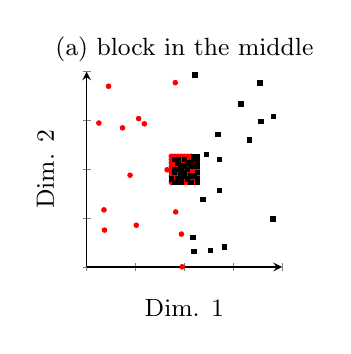
\begin{tikzpicture}

\begin{axis}[
footnotesize,
width= 1.6in,
height= 1.6in,
xmin=0, xmax=30,
ymin=0, ymax=30,
title={(a) block in the middle},
ytick={0,7.5,15,22.5,30},
xtick = {0,7.5,15,22.5,30},
xlabel = {Dim. 1},
ylabel = {Dim. 2},
xticklabels={,,,,},
yticklabels={,,,,},
axis on top,
axis y line = left,
axis x line = bottom
%legend entries={$optimal$,$rand$,$IVM$,$maxent$,$QBC2$,$QBC100$,$SVM$},
 %egend style={nodes=right}
]
\addplot [
color=red,
only marks,
mark=*,
mark options={scale = 0.4}
]
coordinates{ (13,13) (15,13) (15.5,13) (16.5,13) (13.5,13.5) (15,13.5) (16,13.5) (16.5,13.5) (13,14) (13.5,14) (14,14) (15.5,14) (17,14) (13,14.5) (14,14.5) (15.5,14.5) (16,14.5) (16.5,14.5) (13,15) (15,15) (16,15) (16.5,15) (17,15) (13,15.5) (13.5,15.5) (14,15.5) (15.5,15.5) (13,16) (13.5,16) (14.5,16) (15,16) (16.5,16) (13,16.5) (14.5,16.5) (15.5,16.5) (16,16.5) (13,17) (13.5,17) (14,17) (14.5,17) (15,17) (15.5,17) (16,17) (8.86203,21.9844) (1.87844,22.0987) (7.62888,6.41534) (5.50559,21.3585) (7.97933,22.783) (6.66413,14.0934) (2.66314,8.77752) (14.6582,0.0330902) (13.6696,8.46285) (2.74037,5.67331) (13.6087,28.3003) (12.3521,14.9273) (3.36577,27.7504) (14.5511,5.06006)
};
\label{plots:negatives}

\addplot [
color=black,
only marks,
mark=square*,
mark options={scale = 0.4}
]
coordinates{ (13.5,13) (14,13) (14.5,13) (16,13) (17,13) (13,13.5) (14,13.5) (14.5,13.5) (15.5,13.5) (17,13.5) (14.5,14) (15,14) (16,14) (16.5,14) (13.5,14.5) (14.5,14.5) (15,14.5) (17,14.5) (13.5,15) (14,15) (14.5,15) (15.5,15) (14.5,15.5) (15,15.5) (16,15.5) (16.5,15.5) (17,15.5) (14,16) (15.5,16) (16,16) (17,16) (13.5,16.5) (14,16.5) (15,16.5) (16.5,16.5) (17,16.5) (16.5,17) (17,17) (18.3773,17.3043) (24.9794,19.4896) (26.7589,22.3496) (17.8888,10.3495) (16.4577,2.38458) (20.4057,11.7607) (19.0268,2.51172) (20.4262,16.5161) (28.71,23.0737) (21.1403,3.08034) (16.3379,4.55224) (20.1516,20.3166) (23.7032,25.0623) (26.6266,28.273) (16.6152,29.476) (28.6434,7.37318)
};
\label{plots:positives}

\end{axis}
\end{tikzpicture}
&
% This file was created by matlab2tikz v0.0.7.
% Copyright (c) 2008--2010, Nico Schlömer <nico.schloemer@gmail.com>
% All rights reserved.
% 
% The latest updates can be retrieved from
%   http://www.mathworks.com/matlabcentral/fileexchange/22022-matlab2tikz
% where you can also make suggestions and rate matlab2tikz.
% 
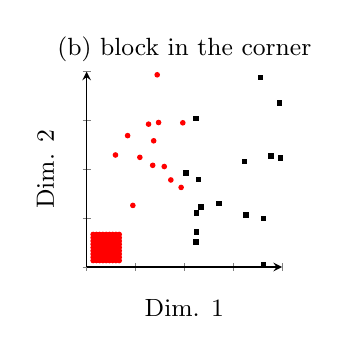
\begin{tikzpicture}

\begin{axis}[
footnotesize,
width= 1.6in,
height= 1.6in,
xmin=0, xmax=30,
ymin=0, ymax=30,
title={(b) block in the corner},
xlabel = {Dim. 1},
ylabel = {Dim. 2},
ytick={0,7.5,15,22.5,30},
xtick = {0,7.5,15,22.5,30},
xticklabels={,,,,},
yticklabels={,,,,},
axis on top,
axis y line = left,
axis x line = bottom
%legend entries={$optimal$,$rand$,$IVM$,$maxent$,$QBC2$,$QBC100$,$SVM$},
 %egend style={nodes=right}
]

\addplot [
color=red,
only marks,
mark=*,
mark options={scale=0.4}
]
coordinates{ (1,1) (1.5,1) (2,1) (2.5,1) (3,1) (3.5,1) (4,1) (4.5,1) (5,1) (1,1.5) (1.5,1.5) (2,1.5) (2.5,1.5) (3,1.5) (3.5,1.5) (4,1.5) (4.5,1.5) (5,1.5) (1,2) (1.5,2) (2,2) (2.5,2) (3,2) (3.5,2) (4,2) (4.5,2) (5,2) (1,2.5) (1.5,2.5) (2,2.5) (2.5,2.5) (3,2.5) (3.5,2.5) (4,2.5) (4.5,2.5) (5,2.5) (1,3) (1.5,3) (2,3) (2.5,3) (3,3) (3.5,3) (4,3) (4.5,3) (5,3) (1,3.5) (1.5,3.5) (2,3.5) (2.5,3.5) (3,3.5) (3.5,3.5) (4,3.5) (4.5,3.5) (5,3.5) (1,4) (1.5,4) (2,4) (2.5,4) (3,4) (3.5,4) (4,4) (4.5,4) (5,4) (1,4.5) (1.5,4.5) (2,4.5) (2.5,4.5) (3,4.5) (3.5,4.5) (4,4.5) (4.5,4.5) (5,4.5) (1,5) (1.5,5) (2,5) (2.5,5) (3,5) (3.5,5) (4,5) (4.5,5) (5,5) (14.7594,22.137) (9.50211,21.9321) (11.9146,15.4247) (4.42475,17.1991) (7.09258,9.45929) (11.0419,22.1845) (14.5021,12.2209) (12.9235,13.3655) (10.8308,29.5065) (10.2906,19.3776) (4.33421,3.57372) (10.1417,15.6132) (6.28981,20.1691) (8.16591,16.8388)
};

\addplot [
color=black,
only marks,
mark=square*,
mark options={scale=0.4}
]
coordinates{ (17.1549,13.4394) (29.7725,16.7571) (16.7772,22.7654) (28.2901,17.0776) (16.8774,8.28907) (17.5203,9.19147) (27.1422,7.43214) (16.8312,5.41786) (20.3286,9.78169) (24.4829,8.00663) (27.1345,0.366002) (29.6109,25.1893) (24.263,16.1932) (15.2474,14.4045) (26.6495,29.111) (16.7822,3.87225)
};

\end{axis}
\end{tikzpicture}
&
% This file was created by matlab2tikz v0.0.7.
% Copyright (c) 2008--2010, Nico Schlömer <nico.schloemer@gmail.com>
% All rights reserved.
% 
% The latest updates can be retrieved from
%   http://www.mathworks.com/matlabcentral/fileexchange/22022-matlab2tikz
% where you can also make suggestions and rate matlab2tikz.
% 
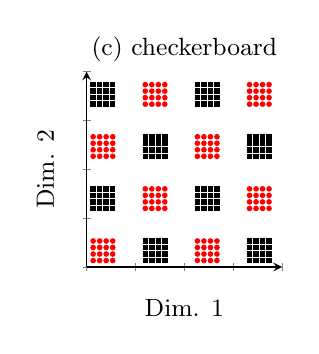
\begin{tikzpicture}

\begin{axis}[
footnotesize,
width= 1.6in,
height= 1.6in,
xmin=0, xmax=30,
ymin=0, ymax=30,
title={(c) checkerboard},
xlabel = {Dim. 1},
ylabel = {Dim. 2},
ytick={0,7.5,15,22.5,30},
xtick = {0,7.5,15,22.5,30},
xticklabels={,,,,},
yticklabels={,,,,},
axis on top,
axis y line = left,
axis x line = bottom
%legend entries={$optimal$,$rand$,$IVM$,$maxent$,$QBC2$,$QBC100$,$SVM$},
 %egend style={nodes=right}
]

\addplot [
color=red,
only marks,
mark=*,
mark options={scale=0.4}
]
coordinates{ (1,1) (2,1) (3,1) (4,1) (17,1) (18,1) (19,1) (20,1) (1,2) (2,2) (3,2) (4,2) (17,2) (18,2) (19,2) (20,2) (1,3) (2,3) (3,3) (4,3) (17,3) (18,3) (19,3) (20,3) (1,4) (2,4) (3,4) (4,4) (17,4) (18,4) (19,4) (20,4) (9,9) (10,9) (11,9) (12,9) (25,9) (26,9) (27,9) (28,9) (9,10) (10,10) (11,10) (12,10) (25,10) (26,10) (27,10) (28,10) (9,11) (10,11) (11,11) (12,11) (25,11) (26,11) (27,11) (28,11) (9,12) (10,12) (11,12) (12,12) (25,12) (26,12) (27,12) (28,12) (1,17) (2,17) (3,17) (4,17) (17,17) (18,17) (19,17) (20,17) (1,18) (2,18) (3,18) (4,18) (17,18) (18,18) (19,18) (20,18) (1,19) (2,19) (3,19) (4,19) (17,19) (18,19) (19,19) (20,19) (1,20) (2,20) (3,20) (4,20) (17,20) (18,20) (19,20) (20,20) (9,25) (10,25) (11,25) (12,25) (25,25) (26,25) (27,25) (28,25) (9,26) (10,26) (11,26) (12,26) (25,26) (26,26) (27,26) (28,26) (9,27) (10,27) (11,27) (12,27) (25,27) (26,27) (27,27) (28,27) (9,28) (10,28) (11,28) (12,28) (25,28) (26,28) (27,28) (28,28)
};

\addplot [
color=black,
only marks,
mark=square*,
mark options={scale=0.4}
]
coordinates{ (9,1) (10,1) (11,1) (12,1) (25,1) (26,1) (27,1) (28,1) (9,2) (10,2) (11,2) (12,2) (25,2) (26,2) (27,2) (28,2) (9,3) (10,3) (11,3) (12,3) (25,3) (26,3) (27,3) (28,3) (9,4) (10,4) (11,4) (12,4) (25,4) (26,4) (27,4) (28,4) (1,9) (2,9) (3,9) (4,9) (17,9) (18,9) (19,9) (20,9) (1,10) (2,10) (3,10) (4,10) (17,10) (18,10) (19,10) (20,10) (1,11) (2,11) (3,11) (4,11) (17,11) (18,11) (19,11) (20,11) (1,12) (2,12) (3,12) (4,12) (17,12) (18,12) (19,12) (20,12) (9,17) (10,17) (11,17) (12,17) (25,17) (26,17) (27,17) (28,17) (9,18) (10,18) (11,18) (12,18) (25,18) (26,18) (27,18) (28,18) (9,19) (10,19) (11,19) (12,19) (25,19) (26,19) (27,19) (28,19) (9,20) (10,20) (11,20) (12,20) (25,20) (26,20) (27,20) (28,20) (1,25) (2,25) (3,25) (4,25) (17,25) (18,25) (19,25) (20,25) (1,26) (2,26) (3,26) (4,26) (17,26) (18,26) (19,26) (20,26) (1,27) (2,27) (3,27) (4,27) (17,27) (18,27) (19,27) (20,27) (1,28) (2,28) (3,28) (4,28) (17,28) (18,28) (19,28) (20,28)
};

\end{axis}
\end{tikzpicture}
\\
% This file was created by matlab2tikz v0.0.7.
% Copyright (c) 2008--2010, Nico Schlömer <nico.schloemer@gmail.com>
% All rights reserved.
% 
% The latest updates can be retrieved from
%   http://www.mathworks.com/matlabcentral/fileexchange/22022-matlab2tikz
% where you can also make suggestions and rate matlab2tikz.
% 
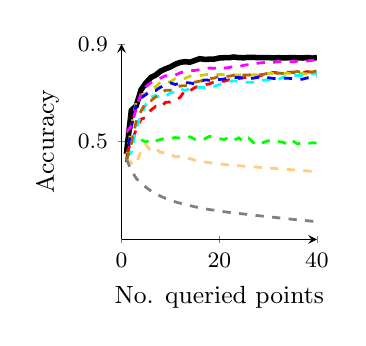
\begin{tikzpicture}

% defining custom colors
\definecolor{mycolor1}{rgb}{0.8,0.8,0}
\definecolor{mycolor2}{rgb}{0,1,1}
\definecolor{mycolor3}{rgb}{1,0,1}
\definecolor{mycolor4}{rgb}{1,0.8,0.5}
\definecolor{mycolor5}{rgb}{0.7,0.4,0.01}


\begin{axis}[
footnotesize,
width= 1.6in,
height= 1.6in,
xmin=0, xmax=40,
ymin=0.1, ymax=0.9,
ytick={0.5,0.9},
xtick = {0,20,40},
xlabel = {No. queried points},
ylabel = {Accuracy},
axis on top,
axis y line = left,
axis x line = bottom
%legend entries={$optimal$,$rand$,$IVM$,$maxent$,$QBC2$,$QBC100$,$SVM$},
 %egend style={nodes=right}
]
\addplot [
color=black,
solid,
line width=2.0pt
]
coordinates{ (1,0.450769) (2,0.627845) (3,0.647265) (4,0.712941) (5,0.741003) (6,0.762954) (7,0.773018) (8,0.789136) (9,0.798441) (10,0.806265) (11,0.817283) (12,0.82484) (13,0.827751) (14,0.825769) (15,0.832678) (16,0.83974) (17,0.837371) (18,0.837804) (19,0.838604) (20,0.842851) (21,0.844002) (22,0.84399) (23,0.846894) (24,0.844338) (25,0.84367) (26,0.845705) (27,0.845233) (28,0.844348) (29,0.844579) (30,0.844709) (31,0.843005) (32,0.844029) (33,0.843528) (34,0.843761) (35,0.84444) (36,0.843425) (37,0.842839) (38,0.844874) (39,0.842366) (40,0.844488)
};
\label{plots:BALD}


\addplot [
color=red,
dashed,
line width=1.0pt
]
coordinates{ (1,0.451086) (2,0.49816) (3,0.549225) (4,0.592272) (5,0.599452) (6,0.629475) (7,0.644924) (8,0.640655) (9,0.66117) (10,0.663051) (11,0.670583) (12,0.681396) (13,0.711317) (14,0.708778) (15,0.721724) (16,0.72956) (17,0.733506) (18,0.736772) (19,0.745888) (20,0.747867) (21,0.74745) (22,0.753887) (23,0.754945) (24,0.758861) (25,0.762162) (26,0.763886) (27,0.764308) (28,0.768394) (29,0.773301) (30,0.775483) (31,0.784175) (32,0.781753) (33,0.781804) (34,0.784162) (35,0.784017) (36,0.78191) (37,0.782467) (38,0.787036) (39,0.784253) (40,0.781836)
};
\label{plots:rand}


\addplot [
color=green,
dashed,
line width=1.0pt
]
coordinates{ (1,0.423574) (2,0.507584) (3,0.493758) (4,0.508564) (5,0.498024) (6,0.511173) (7,0.50287) (8,0.509933) (9,0.514595) (10,0.513477) (11,0.517124) (12,0.514896) (13,0.51485) (14,0.520506) (15,0.510279) (16,0.517637) (17,0.512111) (18,0.522211) (19,0.518124) (20,0.512904) (21,0.509206) (22,0.518069) (23,0.505895) (24,0.515942) (25,0.500831) (26,0.514965) (27,0.496354) (28,0.5073) (29,0.496602) (30,0.504057) (31,0.499562) (32,0.500832) (33,0.498164) (34,0.489265) (35,0.504054) (36,0.491417) (37,0.496447) (38,0.492809) (39,0.495733) (40,0.494792)
};
\label{plots:IVM}


\addplot [
color=mycolor1,
dashed,
line width=1.0pt
]
coordinates{ (1,0.423859) (2,0.560142) (3,0.663338) (4,0.691968) (5,0.697218) (6,0.718702) (7,0.724501) (8,0.744462) (9,0.743842) (10,0.745216) (11,0.758551) (12,0.756943) (13,0.759429) (14,0.768432) (15,0.771157) (16,0.771218) (17,0.773911) (18,0.776606) (19,0.775208) (20,0.775321) (21,0.774416) (22,0.776446) (23,0.773276) (24,0.773258) (25,0.775169) (26,0.772137) (27,0.774075) (28,0.773772) (29,0.775545) (30,0.780022) (31,0.780774) (32,0.780143) (33,0.780392) (34,0.77998) (35,0.780831) (36,0.781354) (37,0.778975) (38,0.777965) (39,0.778391) (40,0.777663)
};
\label{plots:maxent}


\addplot [
color=mycolor2,
dashed,
line width=1.0pt
]
coordinates{ (1,0.437744) (2,0.457254) (3,0.557851) (4,0.607051) (5,0.65399) (6,0.683368) (7,0.689059) (8,0.680439) (9,0.685365) (10,0.699959) (11,0.702562) (12,0.717143) (13,0.709763) (14,0.718033) (15,0.717221) (16,0.72375) (17,0.721815) (18,0.727367) (19,0.727636) (20,0.733762) (21,0.740265) (22,0.747369) (23,0.749206) (24,0.746662) (25,0.744187) (26,0.743369) (27,0.743917) (28,0.745755) (29,0.751835) (30,0.75345) (31,0.754406) (32,0.753725) (33,0.763583) (34,0.768715) (35,0.770087) (36,0.771398) (37,0.7718) (38,0.775158) (39,0.778767) (40,0.78049)
};
\label{plots:QBC2}

\addplot [
color=blue,
dashed,
line width=1.0pt
]
coordinates{ (1,0.417143) (2,0.559673) (3,0.652982) (4,0.679753) (5,0.693065) (6,0.709019) (7,0.710244) (8,0.723463) (9,0.731474) (10,0.741036) (11,0.734572) (12,0.740239) (13,0.741968) (14,0.740834) (15,0.736291) (16,0.746526) (17,0.752956) (18,0.751852) (19,0.75495) (20,0.754615) (21,0.756663) (22,0.762286) (23,0.762192) (24,0.763659) (25,0.759825) (26,0.75857) (27,0.76031) (28,0.763636) (29,0.767371) (30,0.762333) (31,0.759305) (32,0.758561) (33,0.759312) (34,0.760122) (35,0.758054) (36,0.756994) (37,0.755904) (38,0.761444) (39,0.761644) (40,0.765411)
};
\label{plots:QBC100}

\addplot [
color=mycolor3,
dashed,
line width=1.0pt
]
coordinates{ (1,0.5386) (2,0.565211) (3,0.634337) (4,0.700194) (5,0.725775) (6,0.741928) (7,0.752486) (8,0.760961) (9,0.77014) (10,0.767481) (11,0.772995) (12,0.78203) (13,0.788191) (14,0.790413) (15,0.792089) (16,0.794954) (17,0.799203) (18,0.801811) (19,0.800656) (20,0.805692) (21,0.801845) (22,0.803726) (23,0.808346) (24,0.807935) (25,0.812626) (26,0.815763) (27,0.815573) (28,0.822299) (29,0.823795) (30,0.826076) (31,0.825052) (32,0.827026) (33,0.828653) (34,0.828648) (35,0.827402) (36,0.829904) (37,0.82963) (38,0.830456) (39,0.833531) (40,0.836065)
};
\label{plots:SVM}


\addplot [
color=mycolor4,
dashed,
line width=1.0pt
]
coordinates{ (1,0.432646) (2,0.4132) (3,0.40679) (4,0.463525) (5,0.488598) (6,0.462491) (7,0.472777) (8,0.45572) (9,0.45679) (10,0.447679) (11,0.438245) (12,0.440148) (13,0.434083) (14,0.430394) (15,0.424877) (16,0.421133) (17,0.417703) (18,0.414181) (19,0.41102) (20,0.409248) (21,0.407317) (22,0.405129) (23,0.403463) (24,0.401783) (25,0.400397) (26,0.399241) (27,0.397389) (28,0.39576) (29,0.394194) (30,0.392164) (31,0.391381) (32,0.389456) (33,0.387728) (34,0.386783) (35,0.385202) (36,0.383672) (37,0.382133) (38,0.38079) (39,0.378258) (40,0.376427)
};
\label{plots:dec}

\addplot [
color=mycolor5,
dashed,
line width=1.0pt
]
coordinates{ (1,0.423336) (2,0.491499) (3,0.583662) (4,0.625896) (5,0.661889) (6,0.667475) (7,0.683743) (8,0.694363) (9,0.711161) (10,0.711068) (11,0.712454) (12,0.728513) (13,0.729423) (14,0.730234) (15,0.743882) (16,0.748153) (17,0.750597) (18,0.758435) (19,0.760625) (20,0.768514) (21,0.768946) (22,0.767941) (23,0.772845) (24,0.779496) (25,0.772675) (26,0.77328) (27,0.775972) (28,0.773226) (29,0.775773) (30,0.78041) (31,0.779872) (32,0.780489) (33,0.779693) (34,0.780463) (35,0.784821) (36,0.787482) (37,0.784063) (38,0.785672) (39,0.785049) (40,0.791106)
};
\label{plots:semi}


\addplot [
color=gray,
dashed,
line width=1.0pt
]
coordinates{ (1,0.429559) (2,0.382814) (3,0.3505) (4,0.328911) (5,0.313894) (6,0.298766) (7,0.287718) (8,0.277128) (9,0.268509) (10,0.261305) (11,0.254163) (12,0.248497) (13,0.243079) (14,0.238635) (15,0.233852) (16,0.229898) (17,0.225825) (18,0.222464) (19,0.219854) (20,0.216561) (21,0.213598) (22,0.210852) (23,0.208561) (24,0.206426) (25,0.20438) (26,0.202266) (27,0.199495) (28,0.197597) (29,0.195185) (30,0.192938) (31,0.191131) (32,0.189076) (33,0.186821) (34,0.184871) (35,0.182511) (36,0.180476) (37,0.178677) (38,0.176755) (39,0.174803) (40,0.17334)
};
\label{plots:emp}

\end{axis}
\end{tikzpicture}
&
% This file was created by matlab2tikz v0.0.7.
% Copyright (c) 2008--2010, Nico Schlömer <nico.schloemer@gmail.com>
% All rights reserved.
% 
% The latest updates can be retrieved from
%   http://www.mathworks.com/matlabcentral/fileexchange/22022-matlab2tikz
% where you can also make suggestions and rate matlab2tikz.
% 
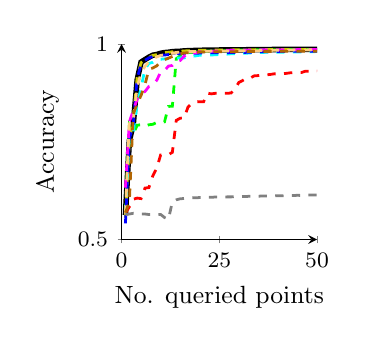
\begin{tikzpicture}

% defining custom colors
\definecolor{mycolor1}{rgb}{0.8,0.8,0}
\definecolor{mycolor2}{rgb}{0,1,1}
\definecolor{mycolor3}{rgb}{1,0,1}
\definecolor{mycolor4}{rgb}{1,0.8,0.5}
\definecolor{mycolor5}{rgb}{0.7,0.4,0.01}


\begin{axis}[
footnotesize,
width= 1.6in,
height= 1.6in,
xmin=0, xmax=50,
ymin=0.5, ymax=1,
xlabel = {No. queried points},
ylabel = {Accuracy},
ytick={0.5,1},
xtick = {0,25,50},
axis on top,
axis y line = left,
axis x line = bottom
%legend entries={$optimal$,$rand$,$IVM$,$maxent$,$QBC2$,$QBC100$,$SVM$},
 %egend style={nodes=right}
]
\addplot [
color=black,
solid,
line width=2.0pt
]
coordinates{ (1,0.562667) (2,0.753156) (3,0.793955) (4,0.908282) (5,0.953695) (6,0.960129) (7,0.966238) (8,0.971448) (9,0.973187) (10,0.976277) (11,0.978092) (12,0.978939) (13,0.980447) (14,0.981087) (15,0.981444) (16,0.982481) (17,0.982896) (18,0.983158) (19,0.9838) (20,0.983895) (21,0.984129) (22,0.984231) (23,0.98438) (24,0.984501) (25,0.984683) (26,0.984824) (27,0.984997) (28,0.985112) (29,0.985063) (30,0.985142) (31,0.985011) (32,0.98537) (33,0.985442) (34,0.985662) (35,0.985525) (36,0.985662) (37,0.985835) (38,0.985905) (39,0.986017) (40,0.98602) (41,0.986079) (42,0.986092) (43,0.986077) (44,0.986192) (45,0.986181) (46,0.986164) (47,0.986202) (48,0.986214) (49,0.986295) (50,0.986152)
};

\addplot [
color=red,
dashed,
line width=1.0pt
]
coordinates{ (1,0.567511) (2,0.583736) (3,0.602877) (4,0.605949) (5,0.604605) (6,0.631527) (7,0.632803) (8,0.662688) (9,0.682383) (10,0.716255) (11,0.716473) (12,0.717064) (13,0.722924) (14,0.80467) (15,0.810332) (16,0.811034) (17,0.838607) (18,0.848563) (19,0.852344) (20,0.852544) (21,0.852496) (22,0.874261) (23,0.87251) (24,0.873947) (25,0.874727) (26,0.873542) (27,0.874193) (28,0.87457) (29,0.885007) (30,0.901715) (31,0.906792) (32,0.913093) (33,0.913468) (34,0.918804) (35,0.91928) (36,0.92072) (37,0.92119) (38,0.922108) (39,0.923704) (40,0.923562) (41,0.924033) (42,0.924796) (43,0.92618) (44,0.92721) (45,0.926867) (46,0.926986) (47,0.930382) (48,0.930175) (49,0.931171) (50,0.931081)
};

\addplot [
color=green,
dashed,
line width=1.0pt
]
coordinates{ (1,0.570195) (2,0.790536) (3,0.769562) (4,0.792235) (5,0.793766) (6,0.789381) (7,0.793477) (8,0.794618) (9,0.799649) (10,0.799764) (11,0.800939) (12,0.840439) (13,0.840839) (14,0.962476) (15,0.969642) (16,0.976745) (17,0.978491) (18,0.978957) (19,0.980398) (20,0.980655) (21,0.981433) (22,0.981854) (23,0.982023) (24,0.982424) (25,0.982585) (26,0.982969) (27,0.983118) (28,0.983722) (29,0.984375) (30,0.984701) (31,0.984823) (32,0.984911) (33,0.985046) (34,0.985125) (35,0.985158) (36,0.985199) (37,0.985316) (38,0.985346) (39,0.985447) (40,0.985536) (41,0.985705) (42,0.985663) (43,0.985744) (44,0.98572) (45,0.985741) (46,0.985801) (47,0.98584) (48,0.985905) (49,0.985902) (50,0.985882)
};

\addplot [
color=mycolor1,
dashed,
line width=1.0pt
]
coordinates{ (1,0.5555) (2,0.752443) (3,0.808389) (4,0.914839) (5,0.952417) (6,0.960066) (7,0.96555) (8,0.970975) (9,0.972806) (10,0.975306) (11,0.977924) (12,0.978673) (13,0.980273) (14,0.980852) (15,0.981352) (16,0.982291) (17,0.982711) (18,0.98324) (19,0.983657) (20,0.983894) (21,0.984238) (22,0.98426) (23,0.984381) (24,0.984398) (25,0.984555) (26,0.984857) (27,0.984992) (28,0.984973) (29,0.985081) (30,0.985062) (31,0.985316) (32,0.985359) (33,0.985607) (34,0.985517) (35,0.985559) (36,0.985728) (37,0.985821) (38,0.985893) (39,0.986032) (40,0.986035) (41,0.985985) (42,0.986138) (43,0.986139) (44,0.986202) (45,0.986182) (46,0.986125) (47,0.98618) (48,0.986219) (49,0.986206) (50,0.986211)
};

\addplot [
color=mycolor2,
dashed,
line width=1.0pt
]
coordinates{ (1,0.567088) (2,0.756156) (3,0.77472) (4,0.84549) (5,0.888183) (6,0.935814) (7,0.950505) (8,0.953254) (9,0.96023) (10,0.961094) (11,0.962025) (12,0.962912) (13,0.963592) (14,0.963964) (15,0.9646) (16,0.964595) (17,0.96811) (18,0.968584) (19,0.969664) (20,0.971402) (21,0.971379) (22,0.971534) (23,0.971959) (24,0.972581) (25,0.973175) (26,0.973403) (27,0.974142) (28,0.974973) (29,0.97531) (30,0.975709) (31,0.976108) (32,0.976562) (33,0.977256) (34,0.978279) (35,0.978259) (36,0.978495) (37,0.978835) (38,0.979033) (39,0.978963) (40,0.979072) (41,0.979226) (42,0.979385) (43,0.979489) (44,0.979539) (45,0.979561) (46,0.979569) (47,0.979883) (48,0.979897) (49,0.980365) (50,0.980764)
};

\addplot [
color=blue,
dashed,
line width=1.0pt
]
coordinates{ (1,0.541424) (2,0.756255) (3,0.795493) (4,0.912543) (5,0.948411) (6,0.958323) (7,0.964496) (8,0.968224) (9,0.970146) (10,0.971164) (11,0.971896) (12,0.973024) (13,0.974036) (14,0.975054) (15,0.975318) (16,0.975498) (17,0.975662) (18,0.976209) (19,0.976408) (20,0.976869) (21,0.977163) (22,0.977486) (23,0.977661) (24,0.977664) (25,0.977685) (26,0.977809) (27,0.977947) (28,0.978116) (29,0.978213) (30,0.978352) (31,0.978303) (32,0.978754) (33,0.978882) (34,0.979323) (35,0.980083) (36,0.98021) (37,0.980292) (38,0.980424) (39,0.980634) (40,0.980771) (41,0.98108) (42,0.981038) (43,0.981107) (44,0.981237) (45,0.981289) (46,0.981433) (47,0.981373) (48,0.981827) (49,0.98176) (50,0.981863)
};

\addplot [
color=mycolor3,
dashed,
line width=1.0pt
]
coordinates{ (1,0.63282) (2,0.800935) (3,0.829853) (4,0.858889) (5,0.87209) (6,0.878661) (7,0.891389) (8,0.895449) (9,0.907277) (10,0.927994) (11,0.932065) (12,0.943548) (13,0.945201) (14,0.955266) (15,0.957909) (16,0.968668) (17,0.975885) (18,0.976961) (19,0.977784) (20,0.980258) (21,0.980665) (22,0.980936) (23,0.981566) (24,0.982013) (25,0.982599) (26,0.983531) (27,0.984044) (28,0.984459) (29,0.983794) (30,0.984794) (31,0.984868) (32,0.984892) (33,0.985008) (34,0.985095) (35,0.985132) (36,0.985239) (37,0.985262) (38,0.985339) (39,0.985378) (40,0.98544) (41,0.985478) (42,0.985559) (43,0.98561) (44,0.985618) (45,0.985677) (46,0.985665) (47,0.985771) (48,0.985762) (49,0.985863) (50,0.985847)
};

\addplot [
color=mycolor4,
dashed,
line width=1.0pt
]
coordinates{ (1,0.566305) (2,0.805511) (3,0.806916) (4,0.890281) (5,0.925929) (6,0.942951) (7,0.954453) (8,0.962239) (9,0.967025) (10,0.970886) (11,0.972673) (12,0.974604) (13,0.97687) (14,0.978388) (15,0.979488) (16,0.979832) (17,0.980456) (18,0.980774) (19,0.981082) (20,0.980673) (21,0.98151) (22,0.981714) (23,0.981879) (24,0.982011) (25,0.982005) (26,0.982162) (27,0.98215) (28,0.98217) (29,0.98237) (30,0.982652) (31,0.982849) (32,0.982782) (33,0.983037) (34,0.983002) (35,0.983031) (36,0.983396) (37,0.98363) (38,0.983661) (39,0.983856) (40,0.983978) (41,0.984125) (42,0.984153) (43,0.984425) (44,0.984461) (45,0.984743) (46,0.984859) (47,0.984994) (48,0.985047) (49,0.98508) (50,0.985148)
};

\addplot [
color=mycolor5,
dashed,
line width=1.0pt
]
coordinates{ (1,0.568585) (2,0.595898) (3,0.821141) (4,0.847498) (5,0.868668) (6,0.895947) (7,0.935528) (8,0.938798) (9,0.944039) (10,0.955205) (11,0.960002) (12,0.963834) (13,0.968172) (14,0.971887) (15,0.974662) (16,0.97714) (17,0.977679) (18,0.978224) (19,0.978781) (20,0.979608) (21,0.979789) (22,0.979978) (23,0.979955) (24,0.980202) (25,0.980297) (26,0.980368) (27,0.980489) (28,0.980387) (29,0.980479) (30,0.980839) (31,0.980877) (32,0.980866) (33,0.981077) (34,0.981198) (35,0.981205) (36,0.981136) (37,0.9812) (38,0.981187) (39,0.981212) (40,0.981213) (41,0.981259) (42,0.981259) (43,0.981284) (44,0.981398) (45,0.98127) (46,0.981704) (47,0.981701) (48,0.981791) (49,0.981785) (50,0.981759)
};

\addplot [
color=gray,
dashed,
line width=1.0pt
]
coordinates{ (1,0.563484) (2,0.565213) (3,0.566948) (4,0.565942) (5,0.564997) (6,0.565225) (7,0.563864) (8,0.563904) (9,0.563406) (10,0.564104) (11,0.55625) (12,0.551891) (13,0.596377) (14,0.601513) (15,0.604207) (16,0.604849) (17,0.605942) (18,0.606736) (19,0.60682) (20,0.607268) (21,0.607367) (22,0.608089) (23,0.607992) (24,0.608661) (25,0.608545) (26,0.608838) (27,0.60902) (28,0.609012) (29,0.609321) (30,0.609589) (31,0.609943) (32,0.610168) (33,0.610655) (34,0.610815) (35,0.610787) (36,0.611186) (37,0.611498) (38,0.61148) (39,0.611688) (40,0.611965) (41,0.611794) (42,0.612583) (43,0.612652) (44,0.612706) (45,0.612973) (46,0.612761) (47,0.613562) (48,0.613595) (49,0.613717) (50,0.613759)
};

\end{axis}
\end{tikzpicture}
&
% This file was created by matlab2tikz v0.0.7.
% Copyright (c) 2008--2010, Nico Schlömer <nico.schloemer@gmail.com>
% All rights reserved.
% 
% The latest updates can be retrieved from
%   http://www.mathworks.com/matlabcentral/fileexchange/22022-matlab2tikz
% where you can also make suggestions and rate matlab2tikz.
% 
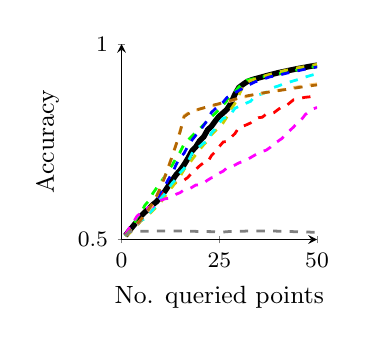
\begin{tikzpicture}


\begin{axis}[
footnotesize,
width= 1.6in,
height= 1.6in,
xmin=0, xmax=50,
ymin=0.5, ymax=1,
ytick={0.5,1},
xtick = {0,25,50},
xlabel = {No. queried points},
ylabel = {Accuracy},
axis on top,
axis y line = left,
axis x line = bottom
%legend entries={$optimal$,$rand$,$IVM$,$maxent$,$QBC2$,$QBC100$,$SVM$},
 %egend style={nodes=right}
]
\addplot [
color=black,
solid,
line width=2.0pt
]
coordinates{ (1,0.509885) (2,0.522693) (3,0.53474) (4,0.547013) (5,0.560323) (6,0.57036) (7,0.57857) (8,0.589043) (9,0.597232) (10,0.609322) (11,0.622262) (12,0.637122) (13,0.651602) (14,0.66623) (15,0.677149) (16,0.691247) (17,0.707813) (18,0.726329) (19,0.736819) (20,0.752558) (21,0.762286) (22,0.780063) (23,0.789513) (24,0.803286) (25,0.815501) (26,0.823959) (27,0.833154) (28,0.848929) (29,0.87118) (30,0.888573) (31,0.896232) (32,0.903101) (33,0.907358) (34,0.910533) (35,0.913087) (36,0.915929) (37,0.918698) (38,0.921288) (39,0.923818) (40,0.926381) (41,0.928526) (42,0.930591) (43,0.932818) (44,0.9349) (45,0.936965) (46,0.938718) (47,0.94052) (48,0.942503) (49,0.944208) (50,0.945905)
};

\addplot [
color=red,
dashed,
line width=1.0pt
]
coordinates{ (1,0.509773) (2,0.519229) (3,0.528577) (4,0.538652) (5,0.548848) (6,0.56459) (7,0.573944) (8,0.588079) (9,0.603113) (10,0.615583) (11,0.624322) (12,0.635052) (13,0.640151) (14,0.646008) (15,0.649586) (16,0.651762) (17,0.659059) (18,0.671112) (19,0.679088) (20,0.688642) (21,0.696339) (22,0.697418) (23,0.714628) (24,0.724863) (25,0.737618) (26,0.749363) (27,0.751161) (28,0.761194) (29,0.770765) (30,0.786319) (31,0.789465) (32,0.793527) (33,0.798071) (34,0.807288) (35,0.81155) (36,0.812729) (37,0.820657) (38,0.821573) (39,0.824516) (40,0.83211) (41,0.839197) (42,0.84107) (43,0.849292) (44,0.857284) (45,0.858584) (46,0.861788) (47,0.863781) (48,0.864775) (49,0.86646) (50,0.867783)
};

\addplot [
color=green,
dashed,
line width=1.0pt
]
coordinates{ (1,0.508449) (2,0.52448) (3,0.534489) (4,0.557607) (5,0.569195) (6,0.587917) (7,0.599197) (8,0.617996) (9,0.632287) (10,0.646611) (11,0.660148) (12,0.676873) (13,0.69087) (14,0.709665) (15,0.723865) (16,0.744137) (17,0.75402) (18,0.764207) (19,0.774987) (20,0.783602) (21,0.7938) (22,0.802727) (23,0.813786) (24,0.822881) (25,0.832758) (26,0.843949) (27,0.855273) (28,0.867317) (29,0.877196) (30,0.889835) (31,0.899085) (32,0.907538) (33,0.909411) (34,0.911749) (35,0.91423) (36,0.916021) (37,0.917998) (38,0.919709) (39,0.922173) (40,0.924) (41,0.925656) (42,0.927179) (43,0.930009) (44,0.93237) (45,0.933966) (46,0.935606) (47,0.937825) (48,0.940095) (49,0.941935) (50,0.943745)
};

\addplot [
color=mycolor1,
dashed,
line width=1.0pt
]
coordinates{ (1,0.508616) (2,0.515568) (3,0.525883) (4,0.537191) (5,0.547513) (6,0.554742) (7,0.564037) (8,0.573611) (9,0.584294) (10,0.594309) (11,0.60828) (12,0.622964) (13,0.634804) (14,0.647751) (15,0.661483) (16,0.67922) (17,0.689835) (18,0.703799) (19,0.716897) (20,0.729839) (21,0.74205) (22,0.752144) (23,0.768311) (24,0.778327) (25,0.786078) (26,0.798597) (27,0.814074) (28,0.833299) (29,0.848099) (30,0.868333) (31,0.89076) (32,0.901281) (33,0.906562) (34,0.90999) (35,0.913697) (36,0.916841) (37,0.919672) (38,0.922692) (39,0.925409) (40,0.928351) (41,0.930613) (42,0.9328) (43,0.934905) (44,0.937044) (45,0.939053) (46,0.940839) (47,0.942414) (48,0.944379) (49,0.94623) (50,0.947845)
};

\addplot [
color=mycolor2,
dashed,
line width=1.0pt
]
coordinates{ (1,0.511368) (2,0.521234) (3,0.534471) (4,0.541192) (5,0.549296) (6,0.55336) (7,0.566196) (8,0.576368) (9,0.590969) (10,0.604769) (11,0.616152) (12,0.631036) (13,0.644519) (14,0.655425) (15,0.671102) (16,0.681668) (17,0.699288) (18,0.719853) (19,0.731265) (20,0.738205) (21,0.746837) (22,0.750747) (23,0.772712) (24,0.783562) (25,0.798642) (26,0.80975) (27,0.812511) (28,0.821576) (29,0.835568) (30,0.840282) (31,0.8442) (32,0.849221) (33,0.853489) (34,0.86456) (35,0.869843) (36,0.872548) (37,0.87679) (38,0.88439) (39,0.889286) (40,0.892362) (41,0.896182) (42,0.900409) (43,0.902785) (44,0.905872) (45,0.908694) (46,0.911805) (47,0.915563) (48,0.918425) (49,0.921418) (50,0.923699)
};

\addplot [
color=blue,
dashed,
line width=1.0pt
]
coordinates{ (1,0.509498) (2,0.519054) (3,0.527929) (4,0.537568) (5,0.551151) (6,0.56285) (7,0.576111) (8,0.592502) (9,0.603575) (10,0.62071) (11,0.634414) (12,0.654218) (13,0.669335) (14,0.692337) (15,0.70947) (16,0.720645) (17,0.739182) (18,0.754014) (19,0.766625) (20,0.777609) (21,0.791608) (22,0.805876) (23,0.825049) (24,0.834503) (25,0.844029) (26,0.851438) (27,0.863511) (28,0.868529) (29,0.875978) (30,0.881048) (31,0.886339) (32,0.892711) (33,0.897363) (34,0.902574) (35,0.90609) (36,0.909593) (37,0.91294) (38,0.916156) (39,0.917961) (40,0.920041) (41,0.922319) (42,0.924864) (43,0.927053) (44,0.929225) (45,0.931453) (46,0.933538) (47,0.935713) (48,0.93771) (49,0.939482) (50,0.941397)
};

\addplot [
color=mycolor3,
dashed,
line width=1.0pt
]
coordinates{ (1,0.51337) (2,0.529771) (3,0.544297) (4,0.560177) (5,0.568214) (6,0.576879) (7,0.582433) (8,0.584435) (9,0.591358) (10,0.599803) (11,0.603702) (12,0.605604) (13,0.610153) (14,0.615944) (15,0.619902) (16,0.627108) (17,0.628215) (18,0.633332) (19,0.639372) (20,0.639883) (21,0.644345) (22,0.651738) (23,0.65781) (24,0.660388) (25,0.669717) (26,0.67488) (27,0.683468) (28,0.686149) (29,0.690429) (30,0.695878) (31,0.699595) (32,0.703835) (33,0.709444) (34,0.715295) (35,0.720755) (36,0.725257) (37,0.72849) (38,0.735388) (39,0.745585) (40,0.751332) (41,0.758135) (42,0.769001) (43,0.77831) (44,0.7876) (45,0.799152) (46,0.80651) (47,0.819522) (48,0.827645) (49,0.833988) (50,0.83782)
};

\addplot [
color=mycolor4,
dashed,
line width=1.0pt
]
coordinates{ (1,0.509503) (2,0.519416) (3,0.529021) (4,0.539572) (5,0.550976) (6,0.562576) (7,0.575101) (8,0.589434) (9,0.611601) (10,0.634933) (11,0.659819) (12,0.686802) (13,0.715388) (14,0.745879) (15,0.779305) (16,0.81661) (17,0.823452) (18,0.828173) (19,0.830868) (20,0.83343) (21,0.836034) (22,0.838609) (23,0.8412) (24,0.843833) (25,0.846406) (26,0.848906) (27,0.851831) (28,0.854557) (29,0.857288) (30,0.860204) (31,0.863002) (32,0.8658) (33,0.867865) (34,0.87011) (35,0.872043) (36,0.874039) (37,0.875788) (38,0.877721) (39,0.879712) (40,0.881449) (41,0.883304) (42,0.884793) (43,0.88689) (44,0.888692) (45,0.890531) (46,0.89233) (47,0.893886) (48,0.895479) (49,0.896751) (50,0.89818)
};

\addplot [
color=mycolor5,
dashed,
line width=1.0pt
]
coordinates{ (1,0.5108) (2,0.519728) (3,0.529965) (4,0.540986) (5,0.551291) (6,0.564799) (7,0.577927) (8,0.594231) (9,0.611973) (10,0.633352) (11,0.658299) (12,0.685346) (13,0.714151) (14,0.743465) (15,0.775744) (16,0.814025) (17,0.821312) (18,0.826681) (19,0.830442) (20,0.833942) (21,0.836694) (22,0.839855) (23,0.842425) (24,0.845011) (25,0.847563) (26,0.850202) (27,0.853042) (28,0.855901) (29,0.858893) (30,0.861653) (31,0.864464) (32,0.867183) (33,0.869036) (34,0.870872) (35,0.872713) (36,0.874727) (37,0.876214) (38,0.877867) (39,0.878996) (40,0.880543) (41,0.882084) (42,0.883558) (43,0.885244) (44,0.886777) (45,0.888309) (46,0.889937) (47,0.891268) (48,0.892703) (49,0.894114) (50,0.895325)
};

\addplot [
color=gray,
dashed,
line width=1.0pt
]
coordinates{ (1,0.509276) (2,0.519678) (3,0.520474) (4,0.520784) (5,0.521128) (6,0.520995) (7,0.521126) (8,0.521426) (9,0.521438) (10,0.521617) (11,0.521681) (12,0.521675) (13,0.521558) (14,0.521564) (15,0.521527) (16,0.521368) (17,0.521186) (18,0.520923) (19,0.520794) (20,0.520524) (21,0.520356) (22,0.520213) (23,0.520105) (24,0.519821) (25,0.519346) (26,0.519055) (27,0.520018) (28,0.520581) (29,0.520693) (30,0.521041) (31,0.521272) (32,0.521516) (33,0.521537) (34,0.521562) (35,0.521635) (36,0.521661) (37,0.521637) (38,0.521593) (39,0.521533) (40,0.521368) (41,0.521099) (42,0.52069) (43,0.520444) (44,0.520095) (45,0.519873) (46,0.519582) (47,0.519396) (48,0.518945) (49,0.518611) (50,0.518228)
};

\end{axis}
\end{tikzpicture}
 \\
\end{tabular}
\end{center}
\caption{\emph{Top:} Artificial datasets used in our evaluation of active learning methods. Exemplars of the two classes are shown with black squares (\ref{plots:positives}) and red circles (\ref{plots:negatives}). \emph{Bottom:} Results of active learning with nine methods: random query (\ref{plots:rand}), \ourmethod (\ref{plots:BALD}),  MES (\ref{plots:maxent}), QBC with the vote criterion with 2 ($\mbox{QBC}_2$, \ref{plots:QBC2}) and 100 ($\mbox{QBC}_{100}$, \ref{plots:QBC100}) committee members, active SVM (\ref{plots:SVM}), IVM (\ref{plots:IVM}), Kapoor \emph{et al.} \cite{kapoor2007} (\ref{plots:dec}), Zhu \emph{et al.} \cite{zhu2003} (\ref{plots:semi}) and empirical error (\ref{plots:emp}).}
\label{fig:artificial}
\end{figure*}

\paragraph{Quantifying Approximation Losses:} To obtain \eqref{eqn:BALD_GPC} we made two approximations: we perform approximate inference ({\scriptsize $\stackrel{1}{\approx}$}), and we approximated the binary entropy of the Gaussian CDF by a squared exponential ({\scriptsize $\stackrel{2}{\approx}$}). Both of these can be substituted with Monte Carlo approximation, enabling us to compute an asymptotically unbiased estimate of the expected information gain. Using extensive Monte Carlo as the `gold standard', we can evaluate how much we loose by applying these approximations. We quantify approximation error as: 

\begin{align}
\frac{ \max_{\x\in\mathcal{P}} I(\x) - I(\argmax_{\x\in\mathcal{P}}\hat{I}(\x)) }{{\max_{\x\in\mathcal{P}}I(\x) }}\cdot 100\% 
\end{align}

where $I$ is the objective computed using Monte Carlo, $\hat{I}$ is the approximate objective. These experiments were run on the \emph{cancer} dataset, results are shown and discussed in Figure \ref{fig:trick}.



\paragraph{Pool based active learning:} We test \ourmethod for GPC and preference learning in the pool-based setting i.e. selecting $x$ values from a fixed set of data-points. We compare to eight other algorithms discussed in this paper: random sampling, MES, QBC, SVM with version space approximation \cite{tong2001}, decision theoretic approaches in \cite{kapoor2007, zhu2003} and directly minimizing expected empirical error (empirical error is not a widely used method, but is included for analysis of \cite{kapoor2007}).

We consider three artificial, but challenging, datasets. The first of which is similar to the \emph{checkerboard} dataset used in \cite{zhu2003}, and is designed to test the algorithm's capabilities to find multiple disjoint islands of points from one class. The second, \emph{block in the corner}, has a block of uninformative points far from the decision boundary, and the third, \emph{block in the middle}, has a block of noisy points on the decision boundary: a strong active learning algorithm should avoid these uninformative regions. The three datasets and results using each algorithm are depicted in Fig. \ref{fig:artificial}.

In addition to this, we present results on 6 UCI binary classification datasets \emph{australia, crabs, vehicle, isolet, cancer} and \emph{wdbc}. \emph{Letter} is a multiclass dataset for which we select hard-to-distinguish letters E vs. F and D vs. P. For preference learning we use the \emph{cpu, cart} and \emph{kinematics} regression datasets \footnote{Data sets at http://www.liacc.up.pt/~ltorgo/Regression/DataSets.html} processed to yield a preference task as described in \cite{chu2005}. Results are plotted in Fig. \ref{fig:BALD_GPC_results}.


\begin{figure*}
\begin{center}
\begin{tabular}{ccc}
% This file was created by matlab2tikz v0.0.7.
% Copyright (c) 2008--2010, Nico Schlömer <nico.schloemer@gmail.com>
% All rights reserved.
% 
% The latest updates can be retrieved from
%   http://www.mathworks.com/matlabcentral/fileexchange/22022-matlab2tikz
% where you can also make suggestions and rate matlab2tikz.
% 
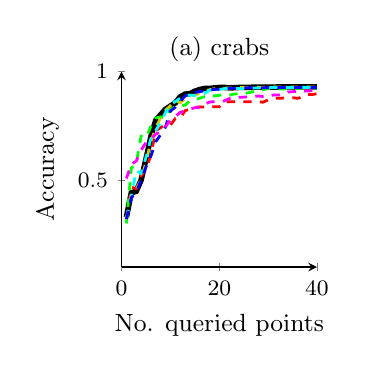
\begin{tikzpicture}

% defining custom colors
\definecolor{mycolor1}{rgb}{0.8,0.8,0}
\definecolor{mycolor2}{rgb}{0,1,1}
\definecolor{mycolor3}{rgb}{1,0,1}


\begin{axis}[
footnotesize,
width= 1.6in,
height= 1.6in,
xmin=0, xmax=40,
ymin=0.1, ymax=1,
ytick={0.5,1},
xtick = {0,20,40},
xlabel = {No. queried points},
ylabel = {Accuracy},
title = {(a) crabs},
axis on top,
axis y line = left,
axis x line = bottom
%legend entries={$optimal$,$rand$,$IVM$,$maxent$,$QBC2$,$QBC100$,$SVM$},
 %egend style={nodes=right}
]
\addplot [
color=black,
solid,
line width=2.0pt
]
coordinates{ (1,0.330028) (2,0.441912) (3,0.448529) (4,0.499924) (5,0.596635) (6,0.700063) (7,0.774983) (8,0.801472) (9,0.826359) (10,0.841491) (11,0.855713) (12,0.883856) (13,0.896074) (14,0.898412) (15,0.909641) (16,0.91707) (17,0.922601) (18,0.922292) (19,0.924926) (20,0.927046) (21,0.926921) (22,0.925409) (23,0.925632) (24,0.926866) (25,0.927044) (26,0.927576) (27,0.927951) (28,0.928284) (29,0.928497) (30,0.928691) (31,0.928805) (32,0.928967) (33,0.929058) (34,0.929171) (35,0.92924) (36,0.929319) (37,0.929392) (38,0.929447) (39,0.929496) (40,0.929527) (41,0.929561) (42,0.929595) (43,0.929626) (44,0.929656) (45,0.929671) (46,0.929697) (47,0.929719) (48,0.929737) (49,0.929763) (50,0.929769) (51,0.929766) (52,0.929802) (53,0.929802) (54,0.929813) (55,0.929822) (56,0.929832) (57,0.929842) (58,0.929859) (59,0.92986) (60,0.929872)
};

\addplot [
color=red,
dashed,
line width=1.0pt
]
coordinates{ (1,0.319793) (2,0.467429) (3,0.461204) (4,0.519779) (5,0.547855) (6,0.614417) (7,0.728458) (8,0.741819) (9,0.756167) (10,0.753366) (11,0.78386) (12,0.784487) (13,0.820005) (14,0.827177) (15,0.83545) (16,0.837616) (17,0.836377) (18,0.839863) (19,0.837948) (20,0.837919) (21,0.861473) (22,0.861215) (23,0.861406) (24,0.862733) (25,0.861122) (26,0.861236) (27,0.860948) (28,0.859857) (29,0.859259) (30,0.869959) (31,0.876097) (32,0.877134) (33,0.877921) (34,0.87974) (35,0.879878) (36,0.877026) (37,0.88189) (38,0.893919) (39,0.894268) (40,0.898019) (41,0.899865) (42,0.900246) (43,0.900758) (44,0.901093) (45,0.906316) (46,0.906792) (47,0.911486) (48,0.910943) (49,0.912668) (50,0.912703) (51,0.914344) (52,0.914384) (53,0.914618) (54,0.91555) (55,0.920038) (56,0.920257) (57,0.922335) (58,0.922763) (59,0.925182) (60,0.924996)
};

\addplot [
color=green,
dashed,
line width=1.0pt
]
coordinates{ (1,0.30069) (2,0.554949) (3,0.575935) (4,0.701644) (5,0.695086) (6,0.747323) (7,0.786041) (8,0.791388) (9,0.787025) (10,0.82541) (11,0.838726) (12,0.842437) (13,0.845102) (14,0.865955) (15,0.869674) (16,0.877434) (17,0.884429) (18,0.885371) (19,0.887891) (20,0.890805) (21,0.895833) (22,0.890647) (23,0.896605) (24,0.898303) (25,0.898572) (26,0.902416) (27,0.908068) (28,0.913104) (29,0.916258) (30,0.921963) (31,0.920936) (32,0.919257) (33,0.920206) (34,0.920769) (35,0.920881) (36,0.923133) (37,0.923456) (38,0.924472) (39,0.924671) (40,0.924737) (41,0.925887) (42,0.926232) (43,0.926503) (44,0.926653) (45,0.9269) (46,0.927624) (47,0.927645) (48,0.928146) (49,0.928384) (50,0.928391) (51,0.928379) (52,0.92858) (53,0.929042) (54,0.92844) (55,0.928136) (56,0.928161) (57,0.928247) (58,0.92828) (59,0.927881) (60,0.927975)
};

\addplot [
color=mycolor1,
dashed,
line width=1.0pt
]
coordinates{ (1,0.322974) (2,0.437443) (3,0.455854) (4,0.504113) (5,0.581877) (6,0.678402) (7,0.740785) (8,0.787365) (9,0.821798) (10,0.842919) (11,0.866204) (12,0.856052) (13,0.875751) (14,0.886431) (15,0.891278) (16,0.900096) (17,0.909833) (18,0.91633) (19,0.921201) (20,0.923789) (21,0.923476) (22,0.924487) (23,0.925499) (24,0.926629) (25,0.926939) (26,0.92733) (27,0.927666) (28,0.927968) (29,0.928283) (30,0.928517) (31,0.92871) (32,0.92884) (33,0.928964) (34,0.929104) (35,0.92921) (36,0.929307) (37,0.929388) (38,0.929427) (39,0.929478) (40,0.929509) (41,0.929555) (42,0.929596) (43,0.929616) (44,0.929648) (45,0.929657) (46,0.929683) (47,0.929655) (48,0.92973) (49,0.929754) (50,0.929764) (51,0.929766) (52,0.929788) (53,0.929791) (54,0.929831) (55,0.92979) (56,0.929846) (57,0.92986) (58,0.92985) (59,0.929866) (60,0.92987)
};

\addplot [
color=mycolor2,
dashed,
line width=1.0pt
]
coordinates{ (1,0.325873) (2,0.420781) (3,0.544173) (4,0.53053) (5,0.604157) (6,0.691406) (7,0.728334) (8,0.765997) (9,0.811855) (10,0.84745) (11,0.861758) (12,0.877297) (13,0.889689) (14,0.891791) (15,0.89015) (16,0.900619) (17,0.899647) (18,0.914089) (19,0.917029) (20,0.917379) (21,0.92142) (22,0.921688) (23,0.921366) (24,0.921837) (25,0.920438) (26,0.921741) (27,0.924229) (28,0.924741) (29,0.925569) (30,0.925966) (31,0.926415) (32,0.926479) (33,0.926532) (34,0.926703) (35,0.92695) (36,0.927102) (37,0.927233) (38,0.927266) (39,0.92739) (40,0.927584) (41,0.927627) (42,0.927678) (43,0.927799) (44,0.927828) (45,0.927861) (46,0.927718) (47,0.927887) (48,0.92803) (49,0.928073) (50,0.928154) (51,0.9282) (52,0.928212) (53,0.928267) (54,0.928264) (55,0.92829) (56,0.928377) (57,0.928508) (58,0.928546) (59,0.928621) (60,0.928674)
};

\addplot [
color=blue,
dashed,
line width=1.0pt
]
coordinates{ (1,0.32095) (2,0.419635) (3,0.443979) (4,0.500687) (5,0.560755) (6,0.61067) (7,0.677272) (8,0.709004) (9,0.744437) (10,0.818105) (11,0.835717) (12,0.862122) (13,0.887368) (14,0.900049) (15,0.903186) (16,0.907917) (17,0.91137) (18,0.91456) (19,0.918803) (20,0.919286) (21,0.922406) (22,0.923135) (23,0.923346) (24,0.925081) (25,0.925548) (26,0.925674) (27,0.925847) (28,0.925932) (29,0.926052) (30,0.926083) (31,0.926195) (32,0.926465) (33,0.926627) (34,0.926839) (35,0.926919) (36,0.927003) (37,0.927079) (38,0.927149) (39,0.927231) (40,0.927278) (41,0.927292) (42,0.927324) (43,0.9274) (44,0.92752) (45,0.927473) (46,0.927559) (47,0.927654) (48,0.927714) (49,0.927765) (50,0.927855) (51,0.927898) (52,0.927915) (53,0.927988) (54,0.928033) (55,0.928053) (56,0.928109) (57,0.928211) (58,0.928261) (59,0.928328) (60,0.928292)
};

\addplot [
color=mycolor3,
dashed,
line width=1.0pt
]
coordinates{ (1,0.507993) (2,0.571946) (3,0.588098) (4,0.637806) (5,0.67307) (6,0.689921) (7,0.712091) (8,0.722253) (9,0.747013) (10,0.776616) (11,0.792642) (12,0.812367) (13,0.818396) (14,0.826281) (15,0.833977) (16,0.834087) (17,0.84945) (18,0.859797) (19,0.861422) (20,0.860765) (21,0.864775) (22,0.875118) (23,0.882063) (24,0.882119) (25,0.88233) (26,0.883771) (27,0.88566) (28,0.887223) (29,0.885073) (30,0.885915) (31,0.891752) (32,0.892311) (33,0.892804) (34,0.905863) (35,0.907591) (36,0.909005) (37,0.910501) (38,0.91077) (39,0.911523) (40,0.913167) (41,0.91433) (42,0.916191) (43,0.915498) (44,0.916049) (45,0.915249) (46,0.916236) (47,0.917819) (48,0.920995) (49,0.921079) (50,0.921158) (51,0.921697) (52,0.920538) (53,0.919319) (54,0.919321) (55,0.919768) (56,0.919819) (57,0.919779) (58,0.920119) (59,0.920323) (60,0.92026)
};

\end{axis}
\end{tikzpicture}
&
% This file was created by matlab2tikz v0.0.7.
% Copyright (c) 2008--2010, Nico Schlömer <nico.schloemer@gmail.com>
% All rights reserved.
% 
% The latest updates can be retrieved from
%   http://www.mathworks.com/matlabcentral/fileexchange/22022-matlab2tikz
% where you can also make suggestions and rate matlab2tikz.
% 
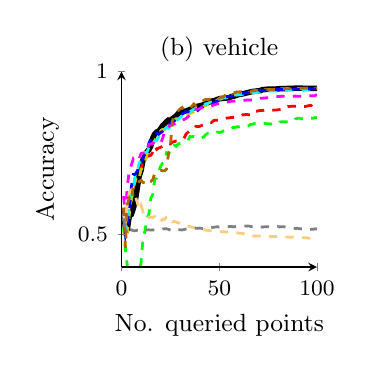
\begin{tikzpicture}




\begin{axis}[
footnotesize,
width= 1.6in,
height= 1.6in,
xmin=0, xmax=100,
ymin=0.4, ymax=1,
xlabel = {No. queried points},
ylabel = {Accuracy},
title={(b) vehicle},
ytick={0.5,1},
xtick = {0,50,100},
axis on top,
axis y line = left,
axis x line = bottom
%legend entries={$optimal$,$rand$,$IVM$,$maxent$,$QBC2$,$QBC100$,$SVM$},
 %egend style={nodes=right}
]
\addplot [
color=black,
solid,
line width=2.0pt
]
coordinates{ (1,0.574487) (2,0.519953) (3,0.519236) (4,0.557799) (5,0.561353) (6,0.579825) (7,0.6029) (8,0.640959) (9,0.678623) (10,0.696683) (11,0.729849) (12,0.740083) (13,0.753396) (14,0.760705) (15,0.771399) (16,0.7961) (17,0.808514) (18,0.814566) (19,0.817034) (20,0.824216) (21,0.833703) (22,0.839305) (23,0.846215) (24,0.850925) (25,0.849674) (26,0.855072) (27,0.859718) (28,0.864089) (29,0.871018) (30,0.873736) (31,0.878886) (32,0.878921) (33,0.8784) (34,0.881275) (35,0.883333) (36,0.885604) (37,0.887822) (38,0.891087) (39,0.893653) (40,0.894626) (41,0.895877) (42,0.899097) (43,0.902486) (44,0.904808) (45,0.906722) (46,0.909494) (47,0.909904) (48,0.911829) (49,0.914586) (50,0.916467) (51,0.917449) (52,0.917529) (53,0.918915) (54,0.918583) (55,0.919133) (56,0.922547) (57,0.924554) (58,0.925207) (59,0.927602) (60,0.929543) (61,0.930394) (62,0.931713) (63,0.932885) (64,0.934587) (65,0.935787) (66,0.937716) (67,0.938778) (68,0.939427) (69,0.940305) (70,0.940946) (71,0.941517) (72,0.944416) (73,0.944849) (74,0.945364) (75,0.94608) (76,0.94609) (77,0.946071) (78,0.946304) (79,0.946346) (80,0.946981) (81,0.947392) (82,0.947623) (83,0.947702) (84,0.947923) (85,0.948174) (86,0.948502) (87,0.948657) (88,0.948744) (89,0.948924) (90,0.949052) (91,0.94921) (92,0.949252) (93,0.947993) (94,0.948528) (95,0.948499) (96,0.948519) (97,0.948585) (98,0.948646) (99,0.948662) (100,0.948711)
};

\addplot [
color=red,
dashed,
line width=1.0pt
]
coordinates{ (1,0.573955) (2,0.517462) (3,0.511933) (4,0.595242) (5,0.609523) (6,0.622966) (7,0.674512) (8,0.682661) (9,0.690525) (10,0.700612) (11,0.725988) (12,0.728277) (13,0.739384) (14,0.741336) (15,0.74329) (16,0.752746) (17,0.771317) (18,0.761218) (19,0.765428) (20,0.767766) (21,0.770192) (22,0.768529) (23,0.771158) (24,0.778663) (25,0.777832) (26,0.783685) (27,0.78502) (28,0.787086) (29,0.787669) (30,0.787666) (31,0.791207) (32,0.795918) (33,0.808139) (34,0.813577) (35,0.820895) (36,0.820282) (37,0.823882) (38,0.831778) (39,0.831309) (40,0.831903) (41,0.834708) (42,0.836776) (43,0.837735) (44,0.841388) (45,0.844961) (46,0.843627) (47,0.849212) (48,0.850829) (49,0.85059) (50,0.851269) (51,0.851682) (52,0.853974) (53,0.856429) (54,0.857528) (55,0.85784) (56,0.859208) (57,0.85917) (58,0.860215) (59,0.86117) (60,0.861874) (61,0.8622) (62,0.867384) (63,0.867876) (64,0.867935) (65,0.867819) (66,0.866892) (67,0.878079) (68,0.877832) (69,0.878147) (70,0.879792) (71,0.88059) (72,0.880262) (73,0.881779) (74,0.882535) (75,0.882801) (76,0.880488) (77,0.880324) (78,0.882146) (79,0.882073) (80,0.882674) (81,0.883606) (82,0.883721) (83,0.883599) (84,0.890623) (85,0.892621) (86,0.893072) (87,0.893481) (88,0.893638) (89,0.893388) (90,0.892284) (91,0.892315) (92,0.892741) (93,0.892909) (94,0.892756) (95,0.894321) (96,0.895625) (97,0.89614) (98,0.902128) (99,0.902208) (100,0.902253)
};

\addplot [
color=green,
dashed,
line width=1.0pt
]
coordinates{ (1,0.522007) (2,0.454272) (3,0.401887) (4,0.389419) (5,0.37767) (6,0.36143) (7,0.348624) (8,0.338585) (9,0.373051) (10,0.415071) (11,0.488982) (12,0.511295) (13,0.549517) (14,0.562798) (15,0.611648) (16,0.623066) (17,0.669598) (18,0.673022) (19,0.691925) (20,0.709374) (21,0.718936) (22,0.723258) (23,0.74963) (24,0.743891) (25,0.763942) (26,0.764739) (27,0.773382) (28,0.770381) (29,0.778012) (30,0.779972) (31,0.782324) (32,0.784405) (33,0.787733) (34,0.788857) (35,0.800682) (36,0.800001) (37,0.80107) (38,0.797757) (39,0.796495) (40,0.794954) (41,0.797516) (42,0.799074) (43,0.806134) (44,0.809837) (45,0.810096) (46,0.810776) (47,0.812461) (48,0.810555) (49,0.814547) (50,0.813343) (51,0.813808) (52,0.817579) (53,0.819515) (54,0.821788) (55,0.822432) (56,0.822301) (57,0.828283) (58,0.828695) (59,0.830396) (60,0.83027) (61,0.832965) (62,0.832612) (63,0.832025) (64,0.831756) (65,0.833739) (66,0.837477) (67,0.838432) (68,0.840478) (69,0.840574) (70,0.84) (71,0.84112) (72,0.841137) (73,0.841429) (74,0.839952) (75,0.839891) (76,0.839493) (77,0.838529) (78,0.838281) (79,0.839026) (80,0.838404) (81,0.845158) (82,0.845876) (83,0.845675) (84,0.845574) (85,0.845801) (86,0.845789) (87,0.846123) (88,0.84743) (89,0.85486) (90,0.856233) (91,0.856905) (92,0.855082) (93,0.855356) (94,0.855711) (95,0.856086) (96,0.856017) (97,0.856421) (98,0.856559) (99,0.858744) (100,0.858212)
};

\addplot [
color=mycolor1,
dashed,
line width=1.0pt
]
coordinates{ (1,0.565168) (2,0.509078) (3,0.508908) (4,0.56191) (5,0.608177) (6,0.646209) (7,0.662318) (8,0.683033) (9,0.675007) (10,0.698982) (11,0.708745) (12,0.719837) (13,0.745147) (14,0.755749) (15,0.776879) (16,0.779344) (17,0.788805) (18,0.798832) (19,0.804859) (20,0.817962) (21,0.822577) (22,0.82171) (23,0.827661) (24,0.831161) (25,0.839299) (26,0.845824) (27,0.851643) (28,0.855474) (29,0.854476) (30,0.857967) (31,0.861351) (32,0.863408) (33,0.868646) (34,0.869131) (35,0.871671) (36,0.873759) (37,0.876538) (38,0.879929) (39,0.881911) (40,0.883855) (41,0.890678) (42,0.894436) (43,0.895534) (44,0.898108) (45,0.899944) (46,0.904897) (47,0.908328) (48,0.909023) (49,0.912671) (50,0.91579) (51,0.917654) (52,0.920515) (53,0.922011) (54,0.924615) (55,0.925719) (56,0.925632) (57,0.926714) (58,0.928221) (59,0.929035) (60,0.931687) (61,0.932256) (62,0.932421) (63,0.934073) (64,0.933582) (65,0.935315) (66,0.936241) (67,0.937659) (68,0.93825) (69,0.939125) (70,0.941515) (71,0.942203) (72,0.942864) (73,0.943714) (74,0.944315) (75,0.944533) (76,0.94507) (77,0.945289) (78,0.945751) (79,0.946183) (80,0.946651) (81,0.94678) (82,0.947053) (83,0.947271) (84,0.947498) (85,0.947966) (86,0.948178) (87,0.948299) (88,0.948637) (89,0.947273) (90,0.94792) (91,0.948119) (92,0.948123) (93,0.948141) (94,0.948197) (95,0.948279) (96,0.948038) (97,0.948247) (98,0.948297) (99,0.948445) (100,0.94854)
};

\addplot [
color=mycolor2,
dashed,
line width=1.0pt
]
coordinates{ (1,0.565905) (2,0.508923) (3,0.543692) (4,0.587811) (5,0.621558) (6,0.650144) (7,0.676025) (8,0.692339) (9,0.719422) (10,0.726345) (11,0.73804) (12,0.751715) (13,0.752468) (14,0.767855) (15,0.767696) (16,0.777108) (17,0.786162) (18,0.78911) (19,0.798874) (20,0.80511) (21,0.818877) (22,0.822836) (23,0.829083) (24,0.825488) (25,0.831292) (26,0.83673) (27,0.843493) (28,0.85024) (29,0.853663) (30,0.859216) (31,0.865186) (32,0.871329) (33,0.874125) (34,0.876369) (35,0.877487) (36,0.880277) (37,0.884732) (38,0.887907) (39,0.888633) (40,0.892481) (41,0.897993) (42,0.898147) (43,0.900947) (44,0.902253) (45,0.905124) (46,0.90602) (47,0.908597) (48,0.910235) (49,0.911281) (50,0.913601) (51,0.916306) (52,0.91866) (53,0.918875) (54,0.920056) (55,0.922966) (56,0.924908) (57,0.925459) (58,0.926693) (59,0.927686) (60,0.928821) (61,0.928504) (62,0.930164) (63,0.933114) (64,0.934276) (65,0.934441) (66,0.934879) (67,0.935391) (68,0.93569) (69,0.935887) (70,0.936234) (71,0.936826) (72,0.937223) (73,0.937612) (74,0.938314) (75,0.939075) (76,0.940165) (77,0.940424) (78,0.940589) (79,0.940625) (80,0.9409) (81,0.941146) (82,0.941719) (83,0.94229) (84,0.94254) (85,0.942748) (86,0.942972) (87,0.943304) (88,0.943437) (89,0.943615) (90,0.943669) (91,0.943883) (92,0.943919) (93,0.943983) (94,0.944002) (95,0.944104) (96,0.944152) (97,0.944212) (98,0.944385) (99,0.944417) (100,0.944463)
};

\addplot [
color=blue,
dashed,
line width=1.0pt
]
coordinates{ (1,0.573021) (2,0.501237) (3,0.537266) (4,0.571499) (5,0.644322) (6,0.683996) (7,0.684478) (8,0.694198) (9,0.707501) (10,0.713141) (11,0.735228) (12,0.74617) (13,0.756248) (14,0.780246) (15,0.793412) (16,0.800365) (17,0.80043) (18,0.809988) (19,0.807566) (20,0.812691) (21,0.816378) (22,0.822969) (23,0.830155) (24,0.835714) (25,0.840755) (26,0.843229) (27,0.848682) (28,0.852822) (29,0.860411) (30,0.865233) (31,0.869899) (32,0.873088) (33,0.87709) (34,0.876518) (35,0.880541) (36,0.879507) (37,0.879272) (38,0.877271) (39,0.8806) (40,0.885164) (41,0.890602) (42,0.893589) (43,0.896114) (44,0.897192) (45,0.89873) (46,0.899168) (47,0.903007) (48,0.906092) (49,0.909672) (50,0.911376) (51,0.915937) (52,0.918885) (53,0.92192) (54,0.922671) (55,0.923938) (56,0.924334) (57,0.925659) (58,0.926166) (59,0.927022) (60,0.929779) (61,0.932239) (62,0.933123) (63,0.934019) (64,0.934862) (65,0.935104) (66,0.935637) (67,0.936643) (68,0.937631) (69,0.938697) (70,0.940269) (71,0.941775) (72,0.942374) (73,0.942538) (74,0.943041) (75,0.943594) (76,0.943823) (77,0.944651) (78,0.944886) (79,0.945113) (80,0.945195) (81,0.945195) (82,0.945368) (83,0.945419) (84,0.945599) (85,0.945751) (86,0.945913) (87,0.946057) (88,0.94609) (89,0.946209) (90,0.946388) (91,0.94645) (92,0.946574) (93,0.946614) (94,0.946723) (95,0.946852) (96,0.946919) (97,0.946963) (98,0.946973) (99,0.947027) (100,0.947095)
};

\addplot [
color=mycolor3,
dashed,
line width=1.0pt
]
coordinates{ (1,0.61753) (2,0.561896) (3,0.651576) (4,0.69566) (5,0.712688) (6,0.7317) (7,0.724378) (8,0.727223) (9,0.73235) (10,0.748453) (11,0.750163) (12,0.751057) (13,0.75179) (14,0.776709) (15,0.777808) (16,0.780203) (17,0.777501) (18,0.776808) (19,0.77589) (20,0.780544) (21,0.79383) (22,0.817831) (23,0.824414) (24,0.830417) (25,0.835049) (26,0.837754) (27,0.838846) (28,0.844472) (29,0.844934) (30,0.84671) (31,0.850757) (32,0.853078) (33,0.856287) (34,0.861509) (35,0.866098) (36,0.868939) (37,0.878538) (38,0.884077) (39,0.88452) (40,0.886381) (41,0.888591) (42,0.889977) (43,0.89089) (44,0.892138) (45,0.893321) (46,0.894095) (47,0.897022) (48,0.898995) (49,0.901355) (50,0.901302) (51,0.904984) (52,0.905271) (53,0.90633) (54,0.906841) (55,0.907976) (56,0.908963) (57,0.909248) (58,0.90941) (59,0.910585) (60,0.911144) (61,0.911165) (62,0.911123) (63,0.911977) (64,0.912429) (65,0.912926) (66,0.912817) (67,0.913084) (68,0.914475) (69,0.915346) (70,0.915792) (71,0.917955) (72,0.918323) (73,0.91866) (74,0.919664) (75,0.919757) (76,0.919507) (77,0.920805) (78,0.922916) (79,0.923594) (80,0.923702) (81,0.923725) (82,0.924107) (83,0.924185) (84,0.923851) (85,0.923868) (86,0.92396) (87,0.923667) (88,0.924539) (89,0.924674) (90,0.924473) (91,0.924536) (92,0.924607) (93,0.924876) (94,0.924954) (95,0.925665) (96,0.925728) (97,0.92576) (98,0.926112) (99,0.926097) (100,0.929797)
};

\addplot [
color=mycolor4,
dashed,
line width=1.0pt
]
coordinates{ (1,0.562416) (2,0.539246) (3,0.602941) (4,0.628129) (5,0.636648) (6,0.631445) (7,0.617227) (8,0.600075) (9,0.57577) (10,0.58942) (11,0.569617) (12,0.573776) (13,0.555785) (14,0.552243) (15,0.552979) (16,0.552275) (17,0.554846) (18,0.542181) (19,0.542458) (20,0.539573) (21,0.546817) (22,0.546103) (23,0.552977) (24,0.555635) (25,0.551618) (26,0.538907) (27,0.539905) (28,0.538018) (29,0.535215) (30,0.534805) (31,0.530328) (32,0.528394) (33,0.528472) (34,0.525787) (35,0.523935) (36,0.52212) (37,0.520801) (38,0.520329) (39,0.521751) (40,0.521086) (41,0.517978) (42,0.515888) (43,0.513335) (44,0.512312) (45,0.512178) (46,0.511259) (47,0.510488) (48,0.509997) (49,0.508584) (50,0.509259) (51,0.508683) (52,0.508707) (53,0.5079) (54,0.507752) (55,0.50931) (56,0.508473) (57,0.507432) (58,0.50672) (59,0.505781) (60,0.50388) (61,0.503482) (62,0.503012) (63,0.500777) (64,0.496541) (65,0.496272) (66,0.495705) (67,0.495723) (68,0.495427) (69,0.495329) (70,0.495202) (71,0.495084) (72,0.494901) (73,0.494668) (74,0.494803) (75,0.494491) (76,0.494157) (77,0.493817) (78,0.494048) (79,0.494057) (80,0.493738) (81,0.493086) (82,0.493147) (83,0.492969) (84,0.492174) (85,0.492234) (86,0.491658) (87,0.49157) (88,0.491566) (89,0.490579) (90,0.490544) (91,0.490407) (92,0.490333) (93,0.489994) (94,0.489826) (95,0.489494) (96,0.488707) (97,0.488448) (98,0.487765) (99,0.487484) (100,0.487369)
};

\addplot [
color=mycolor5,
dashed,
line width=1.0pt
]
coordinates{ (1,0.58263) (2,0.459097) (3,0.592704) (4,0.611954) (5,0.602254) (6,0.646686) (7,0.648986) (8,0.649314) (9,0.662547) (10,0.666544) (11,0.659658) (12,0.658749) (13,0.654295) (14,0.665347) (15,0.663188) (16,0.668586) (17,0.688839) (18,0.695372) (19,0.695318) (20,0.696568) (21,0.695888) (22,0.695384) (23,0.700325) (24,0.748936) (25,0.771235) (26,0.849167) (27,0.860132) (28,0.870586) (29,0.879736) (30,0.885796) (31,0.889941) (32,0.881524) (33,0.886397) (34,0.886613) (35,0.888669) (36,0.893833) (37,0.900454) (38,0.8955) (39,0.900067) (40,0.898439) (41,0.906991) (42,0.911466) (43,0.91451) (44,0.914283) (45,0.915166) (46,0.916865) (47,0.914073) (48,0.91589) (49,0.915576) (50,0.91852) (51,0.921401) (52,0.921485) (53,0.92678) (54,0.928102) (55,0.930526) (56,0.931817) (57,0.934083) (58,0.935409) (59,0.937721) (60,0.937444) (61,0.938369) (62,0.938587) (63,0.939244) (64,0.939822) (65,0.939184) (66,0.939878) (67,0.940679) (68,0.941731) (69,0.942601) (70,0.94251) (71,0.94283) (72,0.943626) (73,0.944133) (74,0.943959) (75,0.944362) (76,0.944556) (77,0.944934) (78,0.945439) (79,0.945544) (80,0.945995) (81,0.946258) (82,0.946213) (83,0.946558) (84,0.947458) (85,0.947531) (86,0.947636) (87,0.947622) (88,0.947666) (89,0.947847) (90,0.948112) (91,0.948564) (92,0.948751) (93,0.948512) (94,0.94872) (95,0.948812) (96,0.948862) (97,0.948966) (98,0.949183) (99,0.949123) (100,0.949073)
};

\addplot [
color=gray,
dashed,
line width=1.0pt
]
coordinates{ (1,0.54918) (2,0.512749) (3,0.514806) (4,0.515736) (5,0.514084) (6,0.511699) (7,0.511219) (8,0.512922) (9,0.512525) (10,0.511976) (11,0.513112) (12,0.514407) (13,0.513965) (14,0.514263) (15,0.513388) (16,0.514181) (17,0.513847) (18,0.513289) (19,0.51267) (20,0.513991) (21,0.516427) (22,0.517416) (23,0.517246) (24,0.516143) (25,0.51296) (26,0.510508) (27,0.510795) (28,0.512036) (29,0.514623) (30,0.514359) (31,0.513825) (32,0.515298) (33,0.51667) (34,0.517352) (35,0.51742) (36,0.517818) (37,0.518667) (38,0.519418) (39,0.518866) (40,0.519618) (41,0.518628) (42,0.518363) (43,0.518409) (44,0.519093) (45,0.520446) (46,0.521526) (47,0.521966) (48,0.523027) (49,0.523673) (50,0.522873) (51,0.523542) (52,0.523554) (53,0.523536) (54,0.523331) (55,0.524336) (56,0.524113) (57,0.524028) (58,0.523968) (59,0.524502) (60,0.525285) (61,0.525965) (62,0.526317) (63,0.526171) (64,0.525506) (65,0.526089) (66,0.524615) (67,0.523972) (68,0.52436) (69,0.52398) (70,0.522443) (71,0.522787) (72,0.522568) (73,0.523508) (74,0.52374) (75,0.523773) (76,0.523179) (77,0.523975) (78,0.524719) (79,0.523977) (80,0.524196) (81,0.523207) (82,0.523705) (83,0.523778) (84,0.522149) (85,0.521023) (86,0.520797) (87,0.520449) (88,0.519427) (89,0.518443) (90,0.518949) (91,0.517514) (92,0.517186) (93,0.517336) (94,0.517729) (95,0.516409) (96,0.515047) (97,0.515856) (98,0.516033) (99,0.517302) (100,0.517022)
};

\end{axis}
\end{tikzpicture}
&
% This file was created by matlab2tikz v0.0.7.
% Copyright (c) 2008--2010, Nico Schlömer <nico.schloemer@gmail.com>
% All rights reserved.
% 
% The latest updates can be retrieved from
%   http://www.mathworks.com/matlabcentral/fileexchange/22022-matlab2tikz
% where you can also make suggestions and rate matlab2tikz.
% 
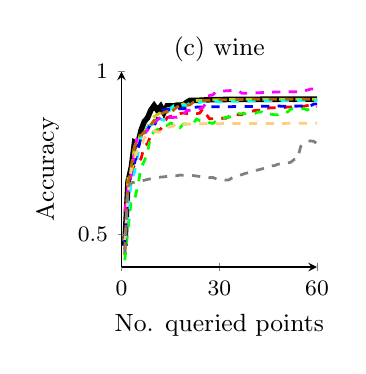
\begin{tikzpicture}

% defining custom colors
\definecolor{mycolor1}{rgb}{0.8,0.8,0}
\definecolor{mycolor2}{rgb}{0,1,1}
\definecolor{mycolor3}{rgb}{1,0,1}
\definecolor{mycolor4}{rgb}{1,0.8,0.5}
\definecolor{mycolor5}{rgb}{0.7,0.4,0.01}


\begin{axis}[
footnotesize,
width= 1.6in,
height= 1.6in,
xmin=0, xmax=60,
ymin=0.4, ymax=1,
title={(c) wine},
xlabel = {No. queried points},
ylabel = {Accuracy},
ytick={0.5,1},
xtick = {0,30,60},
axis on top,
axis y line = left,
axis x line = bottom
%legend entries={$optimal$,$rand$,$IVM$,$maxent$,$QBC2$,$QBC100$,$SVM$},
 %egend style={nodes=right}
]
\addplot [
color=black,
solid,
line width=2.0pt
]
coordinates{ (1,0.465516) (2,0.66236) (3,0.70602) (4,0.783006) (5,0.778101) (6,0.819937) (7,0.846796) (8,0.858126) (9,0.88181) (10,0.895621) (11,0.881396) (12,0.893349) (13,0.874019) (14,0.894958) (15,0.895071) (16,0.89433) (17,0.897117) (18,0.897126) (19,0.898086) (20,0.905681) (21,0.91146) (22,0.911484) (23,0.911696) (24,0.911965) (25,0.912472) (26,0.913053) (27,0.913571) (28,0.913915) (29,0.91402) (30,0.913995) (31,0.914213) (32,0.914304) (33,0.914549) (34,0.914626) (35,0.914647) (36,0.914741) (37,0.914815) (38,0.914776) (39,0.91482) (40,0.914927) (41,0.914955) (42,0.914976) (43,0.915032) (44,0.915055) (45,0.91506) (46,0.915076) (47,0.915093) (48,0.915103) (49,0.915142) (50,0.91514) (51,0.915156) (52,0.915153) (53,0.915097) (54,0.915137) (55,0.915128) (56,0.915122) (57,0.915156) (58,0.915176) (59,0.915168) (60,0.915154)
};

\addplot [
color=red,
dashed,
line width=1.0pt
]
coordinates{ (1,0.437458) (2,0.677661) (3,0.685814) (4,0.715017) (5,0.720606) (6,0.732773) (7,0.772096) (8,0.779033) (9,0.805422) (10,0.811801) (11,0.820256) (12,0.823173) (13,0.840702) (14,0.858805) (15,0.862234) (16,0.863222) (17,0.869481) (18,0.871341) (19,0.872696) (20,0.871295) (21,0.871786) (22,0.872333) (23,0.871298) (24,0.87246) (25,0.886556) (26,0.868624) (27,0.855064) (28,0.855205) (29,0.855322) (30,0.855388) (31,0.856501) (32,0.85648) (33,0.861768) (34,0.861441) (35,0.868783) (36,0.867723) (37,0.867885) (38,0.877485) (39,0.878022) (40,0.87808) (41,0.880723) (42,0.880995) (43,0.881044) (44,0.890131) (45,0.887819) (46,0.889288) (47,0.889142) (48,0.889433) (49,0.889329) (50,0.889777) (51,0.891477) (52,0.89144) (53,0.891937) (54,0.893522) (55,0.893687) (56,0.893474) (57,0.895632) (58,0.896931) (59,0.896984) (60,0.892294)
};

\addplot [
color=green,
dashed,
line width=1.0pt
]
coordinates{ (1,0.420838) (2,0.517416) (3,0.606874) (4,0.606946) (5,0.648919) (6,0.705478) (7,0.725208) (8,0.754642) (9,0.803189) (10,0.815799) (11,0.821905) (12,0.831572) (13,0.834436) (14,0.833836) (15,0.841988) (16,0.839292) (17,0.839918) (18,0.82822) (19,0.838836) (20,0.839067) (21,0.839918) (22,0.840688) (23,0.854183) (24,0.849381) (25,0.849578) (26,0.849004) (27,0.842753) (28,0.840999) (29,0.84731) (30,0.856602) (31,0.856969) (32,0.859386) (33,0.86021) (34,0.860305) (35,0.860298) (36,0.87091) (37,0.870503) (38,0.870221) (39,0.87103) (40,0.871181) (41,0.87188) (42,0.875926) (43,0.876075) (44,0.869114) (45,0.869236) (46,0.869345) (47,0.867494) (48,0.867514) (49,0.874345) (50,0.876196) (51,0.876248) (52,0.885051) (53,0.886067) (54,0.884398) (55,0.88444) (56,0.886405) (57,0.881942) (58,0.887431) (59,0.88807) (60,0.883552)
};

\addplot [
color=mycolor1,
dashed,
line width=1.0pt
]
coordinates{ (1,0.445023) (2,0.671509) (3,0.670662) (4,0.782715) (5,0.781127) (6,0.81586) (7,0.814117) (8,0.830217) (9,0.848957) (10,0.861511) (11,0.867976) (12,0.874274) (13,0.885742) (14,0.886851) (15,0.885483) (16,0.889232) (17,0.900108) (18,0.897372) (19,0.900987) (20,0.89545) (21,0.900326) (22,0.908996) (23,0.911046) (24,0.910877) (25,0.911483) (26,0.912185) (27,0.91286) (28,0.913268) (29,0.913578) (30,0.913793) (31,0.913947) (32,0.913969) (33,0.914162) (34,0.914253) (35,0.914421) (36,0.914426) (37,0.914633) (38,0.914757) (39,0.914832) (40,0.914872) (41,0.914931) (42,0.915005) (43,0.915022) (44,0.915046) (45,0.915071) (46,0.915059) (47,0.915091) (48,0.915123) (49,0.915103) (50,0.915122) (51,0.915114) (52,0.915101) (53,0.915105) (54,0.915147) (55,0.915147) (56,0.915126) (57,0.915141) (58,0.915192) (59,0.915105) (60,0.915164)
};

\addplot [
color=mycolor2,
dashed,
line width=1.0pt
]
coordinates{ (1,0.477472) (2,0.564342) (3,0.665486) (4,0.691343) (5,0.744778) (6,0.804081) (7,0.812779) (8,0.829286) (9,0.835666) (10,0.83907) (11,0.857548) (12,0.85422) (13,0.850409) (14,0.86489) (15,0.88714) (16,0.894932) (17,0.892209) (18,0.897038) (19,0.896479) (20,0.897231) (21,0.903201) (22,0.903371) (23,0.905038) (24,0.905185) (25,0.907945) (26,0.907903) (27,0.907892) (28,0.909365) (29,0.909245) (30,0.907068) (31,0.907471) (32,0.908182) (33,0.908529) (34,0.90921) (35,0.909267) (36,0.90932) (37,0.909311) (38,0.90931) (39,0.909565) (40,0.909809) (41,0.909842) (42,0.910263) (43,0.910218) (44,0.910255) (45,0.910311) (46,0.910324) (47,0.910707) (48,0.910781) (49,0.910612) (50,0.910654) (51,0.91066) (52,0.910846) (53,0.910956) (54,0.910996) (55,0.911167) (56,0.911246) (57,0.911432) (58,0.911552) (59,0.911568) (60,0.911525)
};

\addplot [
color=blue,
dashed,
line width=1.0pt
]
coordinates{ (1,0.464976) (2,0.641995) (3,0.687073) (4,0.719287) (5,0.760701) (6,0.796004) (7,0.809039) (8,0.821083) (9,0.840286) (10,0.83161) (11,0.857084) (12,0.878374) (13,0.882341) (14,0.884507) (15,0.883205) (16,0.883255) (17,0.885344) (18,0.886234) (19,0.886075) (20,0.887494) (21,0.887715) (22,0.889622) (23,0.890888) (24,0.891282) (25,0.891594) (26,0.891728) (27,0.891799) (28,0.89187) (29,0.891935) (30,0.892074) (31,0.892366) (32,0.892289) (33,0.892362) (34,0.8924) (35,0.892571) (36,0.892588) (37,0.892896) (38,0.89289) (39,0.892929) (40,0.892997) (41,0.893069) (42,0.893106) (43,0.893326) (44,0.893405) (45,0.893521) (46,0.893623) (47,0.893729) (48,0.894113) (49,0.893867) (50,0.893873) (51,0.893923) (52,0.893921) (53,0.893945) (54,0.893975) (55,0.894067) (56,0.89427) (57,0.894055) (58,0.894185) (59,0.900676) (60,0.900643)
};

\addplot [
color=mycolor3,
dashed,
line width=1.0pt
]
coordinates{ (1,0.569807) (2,0.642926) (3,0.6856) (4,0.757062) (5,0.80862) (6,0.811352) (7,0.811465) (8,0.821385) (9,0.831948) (10,0.841856) (11,0.851879) (12,0.859384) (13,0.859706) (14,0.859933) (15,0.858864) (16,0.859438) (17,0.85998) (18,0.869316) (19,0.868622) (20,0.880281) (21,0.881147) (22,0.885337) (23,0.886026) (24,0.886091) (25,0.890067) (26,0.904824) (27,0.926497) (28,0.92855) (29,0.937894) (30,0.939453) (31,0.939958) (32,0.940921) (33,0.941274) (34,0.94283) (35,0.942947) (36,0.93988) (37,0.933193) (38,0.933444) (39,0.933571) (40,0.93422) (41,0.934509) (42,0.934915) (43,0.935465) (44,0.935701) (45,0.936051) (46,0.936653) (47,0.937223) (48,0.937171) (49,0.937716) (50,0.938062) (51,0.937775) (52,0.937935) (53,0.938159) (54,0.938218) (55,0.941326) (56,0.941261) (57,0.943067) (58,0.946294) (59,0.946196) (60,0.94629)
};

\addplot [
color=mycolor4,
dashed,
line width=1.0pt
]
coordinates{ (1,0.483329) (2,0.619969) (3,0.709119) (4,0.734739) (5,0.764067) (6,0.771543) (7,0.796007) (8,0.803234) (9,0.811525) (10,0.817891) (11,0.814336) (12,0.815286) (13,0.824242) (14,0.828845) (15,0.830435) (16,0.833336) (17,0.84165) (18,0.843102) (19,0.837705) (20,0.838544) (21,0.839359) (22,0.839286) (23,0.838936) (24,0.839297) (25,0.839841) (26,0.840204) (27,0.840402) (28,0.840348) (29,0.84039) (30,0.839706) (31,0.840453) (32,0.840575) (33,0.84055) (34,0.840781) (35,0.840661) (36,0.840745) (37,0.840729) (38,0.840731) (39,0.840738) (40,0.840834) (41,0.840808) (42,0.840832) (43,0.840827) (44,0.840901) (45,0.840871) (46,0.840941) (47,0.841011) (48,0.840997) (49,0.841031) (50,0.841008) (51,0.841067) (52,0.841148) (53,0.841119) (54,0.841137) (55,0.84116) (56,0.841302) (57,0.841266) (58,0.841275) (59,0.84133) (60,0.841275)
};

\addplot [
color=mycolor5,
dashed,
line width=1.0pt
]
coordinates{ (1,0.452001) (2,0.652074) (3,0.70997) (4,0.770694) (5,0.802676) (6,0.804889) (7,0.814141) (8,0.819575) (9,0.837029) (10,0.85059) (11,0.851159) (12,0.869016) (13,0.874318) (14,0.877955) (15,0.865036) (16,0.882616) (17,0.890443) (18,0.898069) (19,0.8973) (20,0.897239) (21,0.897692) (22,0.905701) (23,0.909072) (24,0.91035) (25,0.911291) (26,0.911592) (27,0.912295) (28,0.91254) (29,0.913085) (30,0.913394) (31,0.913706) (32,0.913715) (33,0.913979) (34,0.914089) (35,0.914275) (36,0.914337) (37,0.914445) (38,0.914474) (39,0.914663) (40,0.914769) (41,0.914819) (42,0.914781) (43,0.914834) (44,0.914833) (45,0.914876) (46,0.914849) (47,0.914944) (48,0.915093) (49,0.91494) (50,0.914934) (51,0.914981) (52,0.914963) (53,0.91498) (54,0.914983) (55,0.914979) (56,0.915005) (57,0.915007) (58,0.914998) (59,0.915018) (60,0.915067)
};

\addplot [
color=gray,
dashed,
line width=1.0pt
]
coordinates{ (1,0.443789) (2,0.647403) (3,0.658687) (4,0.660612) (5,0.663783) (6,0.663898) (7,0.666468) (8,0.669088) (9,0.67098) (10,0.67318) (11,0.67515) (12,0.676168) (13,0.676919) (14,0.678401) (15,0.678379) (16,0.68027) (17,0.680572) (18,0.682424) (19,0.681464) (20,0.681764) (21,0.681485) (22,0.680542) (23,0.679388) (24,0.678057) (25,0.676503) (26,0.675797) (27,0.674398) (28,0.674937) (29,0.671049) (30,0.667731) (31,0.668536) (32,0.667061) (33,0.667652) (34,0.674273) (35,0.676552) (36,0.6811) (37,0.683896) (38,0.687459) (39,0.68976) (40,0.694808) (41,0.696325) (42,0.698253) (43,0.701117) (44,0.703292) (45,0.705859) (46,0.71057) (47,0.711504) (48,0.71555) (49,0.717499) (50,0.717069) (51,0.719154) (52,0.72207) (53,0.730132) (54,0.731576) (55,0.77036) (56,0.780824) (57,0.78522) (58,0.787261) (59,0.785894) (60,0.779016)
};

\end{axis}
\end{tikzpicture}
\\
% This file was created by matlab2tikz v0.0.7.
% Copyright (c) 2008--2010, Nico Schlömer <nico.schloemer@gmail.com>
% All rights reserved.
% 
% The latest updates can be retrieved from
%   http://www.mathworks.com/matlabcentral/fileexchange/22022-matlab2tikz
% where you can also make suggestions and rate matlab2tikz.
% 
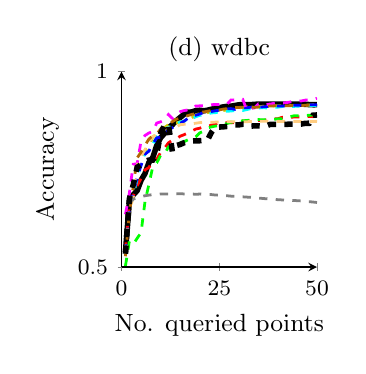
\begin{tikzpicture}

% defining custom colors
\definecolor{mycolor1}{rgb}{0.8,0.8,0}
\definecolor{mycolor2}{rgb}{0,1,1}
\definecolor{mycolor3}{rgb}{1,0,1}
\definecolor{mycolor4}{rgb}{1,0.8,0.5}
\definecolor{mycolor5}{rgb}{0.7,0.4,0.01}


\begin{axis}[
footnotesize,
width= 1.6in,
height= 1.6in,
xmin=0, xmax=50,
ymin=0.5, ymax=1,
title={(d) wdbc},
xlabel = {No. queried points},
ylabel = {Accuracy},
ytick={0.5,1},
xtick = {0,25,50},
axis on top,
axis y line = left,
axis x line = bottom
%legend entries={$optimal$,$rand$,$IVM$,$maxent$,$QBC2$,$QBC100$,$SVM$},
 %egend style={nodes=right}
]
\addplot [
color=black,
solid,
line width=2.0pt
]
coordinates{ (1,0.537981) (2,0.667253) (3,0.685003) (4,0.695484) (5,0.722049) (6,0.739171) (7,0.767443) (8,0.780387) (9,0.810828) (10,0.831055) (11,0.841879) (12,0.85613) (13,0.864001) (14,0.874262) (15,0.882561) (16,0.890716) (17,0.89644) (18,0.896609) (19,0.900273) (20,0.901091) (21,0.899624) (22,0.901253) (23,0.903819) (24,0.906134) (25,0.907536) (26,0.909662) (27,0.911081) (28,0.911541) (29,0.913259) (30,0.915016) (31,0.915524) (32,0.915479) (33,0.915392) (34,0.916158) (35,0.916918) (36,0.916915) (37,0.916384) (38,0.916856) (39,0.916712) (40,0.916593) (41,0.916505) (42,0.916489) (43,0.916682) (44,0.916791) (45,0.916428) (46,0.916509) (47,0.916448) (48,0.915593) (49,0.915139) (50,0.915249)
};

\addplot [
color=red,
dashed,
line width=1.0pt
]
coordinates{ (1,0.541829) (2,0.662297) (3,0.681359) (4,0.708095) (5,0.726384) (6,0.748598) (7,0.754508) (8,0.771781) (9,0.775598) (10,0.793217) (11,0.804005) (12,0.817811) (13,0.824485) (14,0.827845) (15,0.834702) (16,0.838531) (17,0.843385) (18,0.847987) (19,0.853049) (20,0.855136) (21,0.859084) (22,0.860333) (23,0.862753) (24,0.865726) (25,0.86864) (26,0.868144) (27,0.869452) (28,0.868815) (29,0.869751) (30,0.873422) (31,0.873882) (32,0.872187) (33,0.874377) (34,0.874914) (35,0.875045) (36,0.875385) (37,0.876141) (38,0.877799) (39,0.879285) (40,0.879542) (41,0.882824) (42,0.882955) (43,0.88293) (44,0.883581) (45,0.884049) (46,0.884239) (47,0.884794) (48,0.88498) (49,0.884772) (50,0.885541)
};

\addplot [
color=green,
dashed,
line width=1.0pt
]
coordinates{ (1,0.502619) (2,0.565983) (3,0.558757) (4,0.573393) (5,0.588361) (6,0.66731) (7,0.711381) (8,0.756909) (9,0.76633) (10,0.785844) (11,0.788935) (12,0.807289) (13,0.810785) (14,0.813982) (15,0.818375) (16,0.820564) (17,0.825608) (18,0.829551) (19,0.833004) (20,0.843191) (21,0.847517) (22,0.855838) (23,0.858554) (24,0.860562) (25,0.861318) (26,0.865225) (27,0.866948) (28,0.87074) (29,0.869884) (30,0.871686) (31,0.874077) (32,0.874977) (33,0.875717) (34,0.877194) (35,0.877353) (36,0.876431) (37,0.876543) (38,0.878106) (39,0.877955) (40,0.879018) (41,0.879291) (42,0.88061) (43,0.884228) (44,0.886684) (45,0.887018) (46,0.88792) (47,0.887576) (48,0.888277) (49,0.888909) (50,0.889543)
};

\addplot [
color=mycolor1,
dashed,
line width=1.0pt
]
coordinates{ (1,0.535304) (2,0.64962) (3,0.680073) (4,0.731044) (5,0.778285) (6,0.798765) (7,0.807604) (8,0.833686) (9,0.838526) (10,0.849248) (11,0.856833) (12,0.864151) (13,0.867728) (14,0.868633) (15,0.871479) (16,0.873399) (17,0.877009) (18,0.881587) (19,0.889487) (20,0.892456) (21,0.890767) (22,0.89535) (23,0.896597) (24,0.897561) (25,0.898679) (26,0.900247) (27,0.902016) (28,0.904334) (29,0.906273) (30,0.907347) (31,0.908122) (32,0.909368) (33,0.910392) (34,0.911585) (35,0.910665) (36,0.911013) (37,0.911646) (38,0.911693) (39,0.912143) (40,0.912656) (41,0.912664) (42,0.913283) (43,0.913434) (44,0.913408) (45,0.91271) (46,0.91334) (47,0.914093) (48,0.91428) (49,0.915003) (50,0.915139)
};

\addplot [
color=mycolor2,
dashed,
line width=1.0pt
]
coordinates{ (1,0.534646) (2,0.65726) (3,0.6881) (4,0.723802) (5,0.764759) (6,0.790512) (7,0.79676) (8,0.814648) (9,0.832091) (10,0.847065) (11,0.852784) (12,0.857358) (13,0.860684) (14,0.865277) (15,0.871292) (16,0.872839) (17,0.877034) (18,0.879428) (19,0.884346) (20,0.888082) (21,0.888596) (22,0.891602) (23,0.894224) (24,0.894819) (25,0.896949) (26,0.899207) (27,0.898463) (28,0.899114) (29,0.900205) (30,0.901462) (31,0.900351) (32,0.902728) (33,0.905105) (34,0.905204) (35,0.906594) (36,0.907742) (37,0.907047) (38,0.907967) (39,0.908881) (40,0.908962) (41,0.910459) (42,0.910276) (43,0.910811) (44,0.910842) (45,0.911421) (46,0.912084) (47,0.912788) (48,0.912868) (49,0.913204) (50,0.913416)
};

\addplot [
color=blue,
dashed,
line width=1.0pt
]
coordinates{ (1,0.537337) (2,0.64506) (3,0.688151) (4,0.729973) (5,0.759903) (6,0.788575) (7,0.796579) (8,0.815063) (9,0.830454) (10,0.832264) (11,0.841302) (12,0.850667) (13,0.856525) (14,0.864174) (15,0.867784) (16,0.87315) (17,0.880529) (18,0.885292) (19,0.888323) (20,0.891439) (21,0.895417) (22,0.896433) (23,0.89776) (24,0.899824) (25,0.901113) (26,0.903143) (27,0.904691) (28,0.905255) (29,0.903295) (30,0.905399) (31,0.907147) (32,0.907512) (33,0.908802) (34,0.910244) (35,0.909523) (36,0.909642) (37,0.910505) (38,0.911021) (39,0.911292) (40,0.91185) (41,0.912069) (42,0.912234) (43,0.913025) (44,0.913945) (45,0.913986) (46,0.914216) (47,0.914463) (48,0.914947) (49,0.915195) (50,0.915312)
};

\addplot [
color=mycolor3,
dashed,
line width=1.0pt
]
coordinates{ (1,0.634891) (2,0.688896) (3,0.762882) (4,0.764301) (5,0.822706) (6,0.836561) (7,0.842923) (8,0.846616) (9,0.868223) (10,0.871546) (11,0.875555) (12,0.890076) (13,0.880262) (14,0.890869) (15,0.897388) (16,0.900369) (17,0.901862) (18,0.904206) (19,0.911872) (20,0.912364) (21,0.91285) (22,0.91343) (23,0.915408) (24,0.915545) (25,0.91603) (26,0.916451) (27,0.916642) (28,0.927382) (29,0.927681) (30,0.928446) (31,0.928989) (32,0.902567) (33,0.905625) (34,0.907131) (35,0.917371) (36,0.915195) (37,0.915517) (38,0.91707) (39,0.918572) (40,0.91928) (41,0.919534) (42,0.92038) (43,0.92194) (44,0.924428) (45,0.924521) (46,0.924847) (47,0.927009) (48,0.927015) (49,0.927375) (50,0.931873)
};

\addplot [
color=mycolor4,
dashed,
line width=1.0pt
]
coordinates{ (1,0.535716) (2,0.642965) (3,0.679108) (4,0.760866) (5,0.782987) (6,0.800109) (7,0.819669) (8,0.833542) (9,0.839261) (10,0.849802) (11,0.852633) (12,0.855888) (13,0.859039) (14,0.858629) (15,0.864064) (16,0.8651) (17,0.865307) (18,0.866514) (19,0.867869) (20,0.869428) (21,0.870436) (22,0.87106) (23,0.870079) (24,0.870784) (25,0.87098) (26,0.871316) (27,0.871432) (28,0.871438) (29,0.871484) (30,0.87171) (31,0.871215) (32,0.871777) (33,0.872303) (34,0.872894) (35,0.872805) (36,0.872873) (37,0.872846) (38,0.872646) (39,0.872643) (40,0.872619) (41,0.872579) (42,0.872664) (43,0.872559) (44,0.872459) (45,0.872465) (46,0.872507) (47,0.872393) (48,0.872259) (49,0.87218) (50,0.872091)
};

\addplot [
color=mycolor5,
dashed,
line width=1.0pt
]
coordinates{ (1,0.527672) (2,0.637994) (3,0.705762) (4,0.778987) (5,0.794183) (6,0.811297) (7,0.827391) (8,0.83589) (9,0.839802) (10,0.853529) (11,0.858504) (12,0.865165) (13,0.872003) (14,0.878227) (15,0.880739) (16,0.883946) (17,0.887452) (18,0.890535) (19,0.892631) (20,0.895637) (21,0.896665) (22,0.89859) (23,0.900422) (24,0.902215) (25,0.901833) (26,0.904005) (27,0.905312) (28,0.907519) (29,0.907865) (30,0.908354) (31,0.908771) (32,0.90901) (33,0.909729) (34,0.908362) (35,0.909127) (36,0.910216) (37,0.910966) (38,0.911992) (39,0.912329) (40,0.912961) (41,0.913278) (42,0.91261) (43,0.912617) (44,0.913367) (45,0.912832) (46,0.913112) (47,0.913758) (48,0.913602) (49,0.913236) (50,0.91334)
};

\addplot [
color=gray,
dashed,
line width=1.0pt
]
coordinates{ (1,0.535281) (2,0.664101) (3,0.673825) (4,0.676713) (5,0.679949) (6,0.682426) (7,0.683946) (8,0.685287) (9,0.686288) (10,0.68698) (11,0.686783) (12,0.687025) (13,0.687198) (14,0.687187) (15,0.687604) (16,0.687012) (17,0.686924) (18,0.6867) (19,0.686322) (20,0.686627) (21,0.686337) (22,0.685334) (23,0.685326) (24,0.684251) (25,0.683726) (26,0.682901) (27,0.682326) (28,0.681367) (29,0.681241) (30,0.680558) (31,0.679631) (32,0.67895) (33,0.678331) (34,0.677349) (35,0.676457) (36,0.675526) (37,0.674701) (38,0.674122) (39,0.673297) (40,0.672268) (41,0.671752) (42,0.671172) (43,0.670874) (44,0.670153) (45,0.669776) (46,0.669065) (47,0.667961) (48,0.667271) (49,0.666259) (50,0.665147)
};

\addplot [
color=black,
dashed,
line width=2.0pt
]
coordinates{ (1,0.534085) (2,0.674326) (3,0.710569) (4,0.755374) (5,0.761854) (6,0.770103) (7,0.773691) (8,0.773793) (9,0.788584) (10,0.841689) (11,0.863281) (12,0.865411) (13,0.79526) (14,0.810744) (15,0.813542) (16,0.817944) (17,0.820661) (18,0.822134) (19,0.822862) (20,0.823096) (21,0.823788) (22,0.824814) (23,0.844685) (24,0.857666) (25,0.858127) (26,0.858612) (27,0.859711) (28,0.860004) (29,0.863554) (30,0.863663) (31,0.86535) (32,0.865357) (33,0.860502) (34,0.861072) (35,0.861248) (36,0.86097) (37,0.861004) (38,0.864866) (39,0.864986) (40,0.864905) (41,0.864988) (42,0.86505) (43,0.865451) (44,0.865636) (45,0.865644) (46,0.86582) (47,0.867692) (48,0.867849) (49,0.888346) (50,0.889084)
};

\end{axis}
\end{tikzpicture}
&
% This file was created by matlab2tikz v0.0.7.
% Copyright (c) 2008--2010, Nico Schlömer <nico.schloemer@gmail.com>
% All rights reserved.
% 
% The latest updates can be retrieved from
%   http://www.mathworks.com/matlabcentral/fileexchange/22022-matlab2tikz
% where you can also make suggestions and rate matlab2tikz.
% 
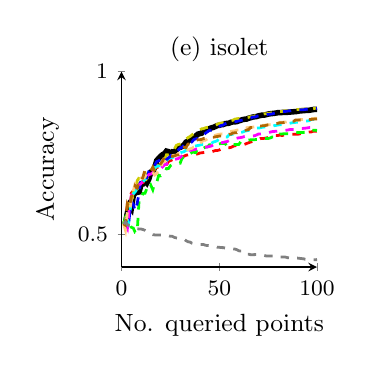
\begin{tikzpicture}



\begin{axis}[
footnotesize,
width= 1.6in,
height= 1.6in,
xmin=0, xmax=100,
ymin=0.4, ymax=1,
title={(e) isolet},
ytick={0.5,1},
xtick = {0,50,100},
xlabel = {No. queried points},
ylabel = {Accuracy},
axis on top,
axis y line = left,
axis x line = bottom
%legend entries={$optimal$,$rand$,$IVM$,$maxent$,$QBC2$,$QBC100$,$SVM$},
 %egend style={nodes=right}
]

\addplot [
color=black,
solid,
line width=2.0pt
]
coordinates{ (1,0.53248) (2,0.534208) (3,0.567173) (4,0.58782) (5,0.579523) (6,0.618814) (7,0.62835) (8,0.628923) (9,0.630519) (10,0.654031) (11,0.655105) (12,0.667098) (13,0.658996) (14,0.670925) (15,0.691714) (16,0.694463) (17,0.705519) (18,0.726861) (19,0.733669) (20,0.740003) (21,0.745111) (22,0.747847) (23,0.755856) (24,0.754296) (25,0.748013) (26,0.753634) (27,0.752526) (28,0.759639) (29,0.765669) (30,0.76747) (31,0.77005) (32,0.774922) (33,0.783497) (34,0.786039) (35,0.792112) (36,0.796416) (37,0.798668) (38,0.802193) (39,0.807672) (40,0.809547) (41,0.81105) (42,0.819232) (43,0.819971) (44,0.82149) (45,0.824919) (46,0.827256) (47,0.828771) (48,0.831309) (49,0.834397) (50,0.834846) (51,0.837097) (52,0.837383) (53,0.840079) (54,0.840908) (55,0.841559) (56,0.84429) (57,0.845607) (58,0.845548) (59,0.846539) (60,0.848755) (61,0.850568) (62,0.852714) (63,0.853689) (64,0.854313) (65,0.856898) (66,0.858265) (67,0.860256) (68,0.861197) (69,0.861828) (70,0.863863) (71,0.865271) (72,0.866335) (73,0.86629) (74,0.867922) (75,0.869486) (76,0.870435) (77,0.87117) (78,0.871804) (79,0.872762) (80,0.873799) (81,0.873757) (82,0.874358) (83,0.874652) (84,0.875049) (85,0.875111) (86,0.875709) (87,0.876069) (88,0.876648) (89,0.876956) (90,0.877917) (91,0.879127) (92,0.879692) (93,0.879924) (94,0.880625) (95,0.880897) (96,0.881261) (97,0.882286) (98,0.88351) (99,0.883823) (100,0.884224)
};

\addplot [
color=red,
dashed,
line width=1.0pt
]
coordinates{ (1,0.532383) (2,0.530488) (3,0.596727) (4,0.609297) (5,0.626968) (6,0.633851) (7,0.637541) (8,0.640254) (9,0.652547) (10,0.657879) (11,0.658994) (12,0.671673) (13,0.674861) (14,0.694531) (15,0.696525) (16,0.701679) (17,0.704008) (18,0.705399) (19,0.707685) (20,0.710429) (21,0.711028) (22,0.713479) (23,0.714672) (24,0.723674) (25,0.726681) (26,0.729408) (27,0.729493) (28,0.730571) (29,0.734141) (30,0.736828) (31,0.737645) (32,0.740227) (33,0.743295) (34,0.744125) (35,0.745576) (36,0.745655) (37,0.744319) (38,0.746176) (39,0.747213) (40,0.750031) (41,0.750697) (42,0.751544) (43,0.752455) (44,0.752649) (45,0.753554) (46,0.753622) (47,0.755531) (48,0.757548) (49,0.757836) (50,0.759285) (51,0.762288) (52,0.762749) (53,0.764846) (54,0.766079) (55,0.766242) (56,0.767303) (57,0.770425) (58,0.772432) (59,0.773145) (60,0.773615) (61,0.774351) (62,0.774537) (63,0.776641) (64,0.779315) (65,0.781423) (66,0.7837) (67,0.785426) (68,0.786128) (69,0.790675) (70,0.791519) (71,0.79439) (72,0.79439) (73,0.795061) (74,0.796088) (75,0.797707) (76,0.800653) (77,0.80323) (78,0.803447) (79,0.803447) (80,0.803932) (81,0.804812) (82,0.804004) (83,0.804421) (84,0.804529) (85,0.805677) (86,0.80626) (87,0.80757) (88,0.807582) (89,0.807665) (90,0.807694) (91,0.808309) (92,0.810727) (93,0.812506) (94,0.81344) (95,0.813822) (96,0.814486) (97,0.814625) (98,0.816646) (99,0.816654) (100,0.816717)
};

\addplot [
color=green,
dashed,
line width=1.0pt
]
coordinates{ (1,0.532449) (2,0.551789) (3,0.540511) (4,0.533481) (5,0.52213) (6,0.519695) (7,0.506214) (8,0.506084) (9,0.607702) (10,0.607388) (11,0.626123) (12,0.626308) (13,0.641965) (14,0.635836) (15,0.650717) (16,0.637142) (17,0.658594) (18,0.658503) (19,0.682134) (20,0.680141) (21,0.687039) (22,0.688) (23,0.702352) (24,0.702284) (25,0.711145) (26,0.714785) (27,0.716423) (28,0.716506) (29,0.71843) (30,0.718784) (31,0.735192) (32,0.735492) (33,0.742883) (34,0.743294) (35,0.747027) (36,0.751889) (37,0.752259) (38,0.751202) (39,0.765096) (40,0.76408) (41,0.764942) (42,0.765006) (43,0.768387) (44,0.768775) (45,0.775607) (46,0.776058) (47,0.776185) (48,0.776284) (49,0.776388) (50,0.777921) (51,0.779375) (52,0.779191) (53,0.779192) (54,0.770934) (55,0.775008) (56,0.774327) (57,0.77633) (58,0.776008) (59,0.776292) (60,0.77642) (61,0.784649) (62,0.787661) (63,0.787662) (64,0.788029) (65,0.789688) (66,0.79042) (67,0.790726) (68,0.790773) (69,0.791675) (70,0.791473) (71,0.792318) (72,0.79311) (73,0.794488) (74,0.794538) (75,0.794543) (76,0.796057) (77,0.798807) (78,0.798976) (79,0.799101) (80,0.799114) (81,0.808384) (82,0.808672) (83,0.808881) (84,0.80907) (85,0.809092) (86,0.809209) (87,0.810589) (88,0.810642) (89,0.811757) (90,0.812908) (91,0.813283) (92,0.81333) (93,0.813333) (94,0.813458) (95,0.817311) (96,0.817988) (97,0.819382) (98,0.819675) (99,0.819677) (100,0.819455)
};

\addplot [
color=mycolor1,
dashed,
line width=1.0pt
]
coordinates{ (1,0.532512) (2,0.54226) (3,0.591607) (4,0.595096) (5,0.585556) (6,0.633198) (7,0.633219) (8,0.664831) (9,0.67437) (10,0.68956) (11,0.68984) (12,0.690042) (13,0.671891) (14,0.67963) (15,0.691186) (16,0.693224) (17,0.701246) (18,0.712453) (19,0.716017) (20,0.716846) (21,0.719888) (22,0.727566) (23,0.744621) (24,0.744367) (25,0.748063) (26,0.752936) (27,0.761859) (28,0.773218) (29,0.776145) (30,0.77751) (31,0.778459) (32,0.787051) (33,0.792967) (34,0.797142) (35,0.800569) (36,0.805418) (37,0.810181) (38,0.810646) (39,0.814567) (40,0.820583) (41,0.82425) (42,0.824982) (43,0.82766) (44,0.828743) (45,0.829573) (46,0.831588) (47,0.832439) (48,0.836115) (49,0.837963) (50,0.840968) (51,0.841732) (52,0.842845) (53,0.84378) (54,0.847455) (55,0.847456) (56,0.849382) (57,0.850843) (58,0.854139) (59,0.855068) (60,0.856288) (61,0.856068) (62,0.856651) (63,0.857591) (64,0.858683) (65,0.859585) (66,0.86168) (67,0.86138) (68,0.863893) (69,0.865791) (70,0.867476) (71,0.867624) (72,0.868595) (73,0.870303) (74,0.870571) (75,0.871173) (76,0.872445) (77,0.873461) (78,0.874381) (79,0.876003) (80,0.876828) (81,0.877087) (82,0.877405) (83,0.878997) (84,0.879528) (85,0.880036) (86,0.881181) (87,0.881715) (88,0.882798) (89,0.883137) (90,0.883716) (91,0.884066) (92,0.884429) (93,0.884688) (94,0.88499) (95,0.885236) (96,0.885737) (97,0.886003) (98,0.886212) (99,0.887186) (100,0.887512)
};

\addplot [
color=mycolor2,
dashed,
line width=1.0pt
]
coordinates{ (1,0.532389) (2,0.537047) (3,0.50815) (4,0.55262) (5,0.604604) (6,0.624475) (7,0.631123) (8,0.639264) (9,0.645182) (10,0.657422) (11,0.661569) (12,0.668595) (13,0.680247) (14,0.681001) (15,0.688697) (16,0.695552) (17,0.704496) (18,0.709591) (19,0.709893) (20,0.712507) (21,0.72137) (22,0.723304) (23,0.726834) (24,0.732178) (25,0.734416) (26,0.73609) (27,0.73851) (28,0.740421) (29,0.748285) (30,0.751236) (31,0.752453) (32,0.754041) (33,0.758815) (34,0.758982) (35,0.765334) (36,0.769315) (37,0.770884) (38,0.771767) (39,0.772993) (40,0.774203) (41,0.776126) (42,0.77647) (43,0.77771) (44,0.778047) (45,0.779299) (46,0.780084) (47,0.783651) (48,0.785584) (49,0.787671) (50,0.795945) (51,0.797856) (52,0.798817) (53,0.799037) (54,0.79902) (55,0.805578) (56,0.806983) (57,0.807647) (58,0.810099) (59,0.812353) (60,0.814202) (61,0.813547) (62,0.814275) (63,0.817098) (64,0.818345) (65,0.819261) (66,0.821854) (67,0.822197) (68,0.824732) (69,0.826556) (70,0.826778) (71,0.82738) (72,0.829341) (73,0.829671) (74,0.830539) (75,0.830926) (76,0.831718) (77,0.831954) (78,0.833965) (79,0.834701) (80,0.836171) (81,0.83662) (82,0.836853) (83,0.83704) (84,0.837435) (85,0.840169) (86,0.841322) (87,0.842421) (88,0.843537) (89,0.844121) (90,0.8445) (91,0.845024) (92,0.845316) (93,0.847593) (94,0.848245) (95,0.848374) (96,0.849198) (97,0.852788) (98,0.853243) (99,0.855758) (100,0.857854)
};

\addplot [
color=blue,
dashed,
line width=1.0pt
]
coordinates{ (1,0.532421) (2,0.536204) (3,0.568549) (4,0.554158) (5,0.601658) (6,0.592596) (7,0.572268) (8,0.595233) (9,0.628393) (10,0.670144) (11,0.670453) (12,0.679957) (13,0.675029) (14,0.69395) (15,0.697914) (16,0.700595) (17,0.712721) (18,0.723513) (19,0.72607) (20,0.729642) (21,0.720804) (22,0.722123) (23,0.730205) (24,0.735128) (25,0.739494) (26,0.752507) (27,0.751848) (28,0.753446) (29,0.758913) (30,0.76549) (31,0.767615) (32,0.774069) (33,0.780804) (34,0.779447) (35,0.782307) (36,0.784012) (37,0.791324) (38,0.793666) (39,0.795149) (40,0.801615) (41,0.804677) (42,0.805215) (43,0.811018) (44,0.815578) (45,0.819603) (46,0.820153) (47,0.82144) (48,0.825674) (49,0.827018) (50,0.831419) (51,0.834611) (52,0.835835) (53,0.839897) (54,0.842244) (55,0.842606) (56,0.844458) (57,0.845094) (58,0.845942) (59,0.847158) (60,0.848391) (61,0.850085) (62,0.851441) (63,0.852991) (64,0.854129) (65,0.85497) (66,0.856876) (67,0.860299) (68,0.860216) (69,0.862233) (70,0.864005) (71,0.864854) (72,0.866448) (73,0.867333) (74,0.867822) (75,0.868989) (76,0.869249) (77,0.870035) (78,0.871861) (79,0.872917) (80,0.874089) (81,0.875084) (82,0.876672) (83,0.877242) (84,0.877806) (85,0.878931) (86,0.879322) (87,0.879888) (88,0.880031) (89,0.880695) (90,0.881638) (91,0.882531) (92,0.882706) (93,0.882861) (94,0.883842) (95,0.884239) (96,0.884656) (97,0.885206) (98,0.885671) (99,0.886151) (100,0.886527)
};

\addplot [
color=mycolor3,
dashed,
line width=1.0pt
]
coordinates{ (1,0.531884) (2,0.530569) (3,0.518269) (4,0.582612) (5,0.619847) (6,0.632239) (7,0.638085) (8,0.649966) (9,0.652545) (10,0.65655) (11,0.663343) (12,0.66451) (13,0.676913) (14,0.683863) (15,0.685436) (16,0.689793) (17,0.695426) (18,0.696367) (19,0.698699) (20,0.700323) (21,0.707822) (22,0.713904) (23,0.716534) (24,0.718935) (25,0.72509) (26,0.725606) (27,0.730257) (28,0.731558) (29,0.733189) (30,0.736127) (31,0.742013) (32,0.746189) (33,0.749975) (34,0.755773) (35,0.758409) (36,0.758932) (37,0.760286) (38,0.761765) (39,0.762745) (40,0.764239) (41,0.765872) (42,0.766556) (43,0.767418) (44,0.769075) (45,0.770155) (46,0.771601) (47,0.775184) (48,0.778636) (49,0.780823) (50,0.78126) (51,0.781476) (52,0.782435) (53,0.78429) (54,0.785224) (55,0.788352) (56,0.791643) (57,0.793509) (58,0.793985) (59,0.795471) (60,0.796686) (61,0.797517) (62,0.79891) (63,0.800992) (64,0.801547) (65,0.801723) (66,0.801859) (67,0.802281) (68,0.803004) (69,0.805154) (70,0.80809) (71,0.808532) (72,0.809254) (73,0.809514) (74,0.810482) (75,0.812258) (76,0.813999) (77,0.81562) (78,0.816329) (79,0.816647) (80,0.816983) (81,0.817507) (82,0.818488) (83,0.819144) (84,0.819666) (85,0.820716) (86,0.821923) (87,0.822448) (88,0.822459) (89,0.822649) (90,0.823129) (91,0.824214) (92,0.825384) (93,0.825656) (94,0.82624) (95,0.827078) (96,0.828005) (97,0.828058) (98,0.828819) (99,0.829992) (100,0.830291)
};

\addplot [
color=mycolor4,
dashed,
line width=1.0pt
]
coordinates{ (1,0.532526) (2,0.512704) (3,0.571136) (4,0.567758) (5,0.604435) (6,0.634246) (7,0.656362) (8,0.653913) (9,0.656394) (10,0.672737) (11,0.672081) (12,0.676239) (13,0.691349) (14,0.690389) (15,0.692502) (16,0.690915) (17,0.682587) (18,0.686694) (19,0.702428) (20,0.700602) (21,0.723396) (22,0.723701) (23,0.732835) (24,0.732075) (25,0.738935) (26,0.741888) (27,0.743366) (28,0.743263) (29,0.74813) (30,0.746817) (31,0.751813) (32,0.754794) (33,0.759831) (34,0.759774) (35,0.763023) (36,0.764246) (37,0.76824) (38,0.769726) (39,0.769603) (40,0.779187) (41,0.783838) (42,0.789091) (43,0.78955) (44,0.794204) (45,0.795438) (46,0.802256) (47,0.802526) (48,0.804696) (49,0.806386) (50,0.807654) (51,0.80861) (52,0.808945) (53,0.812784) (54,0.81355) (55,0.814979) (56,0.816265) (57,0.817561) (58,0.818419) (59,0.820318) (60,0.820632) (61,0.821938) (62,0.822492) (63,0.822582) (64,0.827342) (65,0.828368) (66,0.829083) (67,0.829359) (68,0.830443) (69,0.830618) (70,0.831123) (71,0.832882) (72,0.835033) (73,0.835354) (74,0.836155) (75,0.836482) (76,0.837112) (77,0.837441) (78,0.838462) (79,0.839733) (80,0.840475) (81,0.844499) (82,0.84464) (83,0.844884) (84,0.844919) (85,0.846403) (86,0.847469) (87,0.847536) (88,0.850337) (89,0.850345) (90,0.850351) (91,0.8524) (92,0.852621) (93,0.853108) (94,0.854675) (95,0.85487) (96,0.854931) (97,0.855597) (98,0.855838) (99,0.856593) (100,0.856593)
};

\addplot [
color=mycolor5,
dashed,
line width=1.0pt
]
coordinates{ (1,0.532553) (2,0.528587) (3,0.593105) (4,0.581109) (5,0.616688) (6,0.620919) (7,0.649192) (8,0.642622) (9,0.662915) (10,0.660683) (11,0.677249) (12,0.698189) (13,0.695953) (14,0.698031) (15,0.695008) (16,0.707073) (17,0.694854) (18,0.696485) (19,0.706863) (20,0.717319) (21,0.7251) (22,0.739131) (23,0.737939) (24,0.736217) (25,0.738365) (26,0.739888) (27,0.740812) (28,0.743677) (29,0.743646) (30,0.747566) (31,0.763671) (32,0.767411) (33,0.766949) (34,0.777468) (35,0.77845) (36,0.784055) (37,0.785807) (38,0.789104) (39,0.790463) (40,0.790693) (41,0.791971) (42,0.794609) (43,0.795487) (44,0.796633) (45,0.797538) (46,0.797833) (47,0.798412) (48,0.79974) (49,0.800764) (50,0.802018) (51,0.802483) (52,0.802959) (53,0.803741) (54,0.804061) (55,0.807727) (56,0.807941) (57,0.811647) (58,0.811911) (59,0.812064) (60,0.816372) (61,0.818615) (62,0.819145) (63,0.819678) (64,0.820448) (65,0.822036) (66,0.828241) (67,0.82846) (68,0.831361) (69,0.831507) (70,0.832449) (71,0.832537) (72,0.833463) (73,0.833601) (74,0.835073) (75,0.836742) (76,0.836803) (77,0.839783) (78,0.840114) (79,0.840762) (80,0.841141) (81,0.842716) (82,0.842857) (83,0.843533) (84,0.845025) (85,0.846108) (86,0.847337) (87,0.847342) (88,0.847348) (89,0.851213) (90,0.851259) (91,0.851402) (92,0.852002) (93,0.852273) (94,0.852329) (95,0.852522) (96,0.852627) (97,0.852991) (98,0.853834) (99,0.85431) (100,0.854454)
};

\addplot [
color=gray,
dashed,
line width=1.0pt
]
coordinates{ (1,0.532542) (2,0.537909) (3,0.530471) (4,0.527358) (5,0.52588) (6,0.523191) (7,0.520468) (8,0.517579) (9,0.516854) (10,0.516583) (11,0.515229) (12,0.512552) (13,0.508387) (14,0.504262) (15,0.501699) (16,0.499321) (17,0.498721) (18,0.498526) (19,0.498198) (20,0.498248) (21,0.497954) (22,0.497276) (23,0.496789) (24,0.49642) (25,0.494405) (26,0.494218) (27,0.491106) (28,0.489523) (29,0.488973) (30,0.488481) (31,0.487216) (32,0.485613) (33,0.480904) (34,0.477745) (35,0.476724) (36,0.473244) (37,0.471917) (38,0.470811) (39,0.469806) (40,0.469428) (41,0.46936) (42,0.469035) (43,0.46671) (44,0.466191) (45,0.465866) (46,0.464454) (47,0.463162) (48,0.463111) (49,0.46092) (50,0.460596) (51,0.459678) (52,0.459613) (53,0.458333) (54,0.458145) (55,0.456803) (56,0.456841) (57,0.455804) (58,0.455238) (59,0.453321) (60,0.449977) (61,0.449143) (62,0.449305) (63,0.448732) (64,0.439842) (65,0.439453) (66,0.438013) (67,0.438093) (68,0.438125) (69,0.438341) (70,0.436266) (71,0.436235) (72,0.435643) (73,0.43561) (74,0.434032) (75,0.434058) (76,0.433844) (77,0.433853) (78,0.433887) (79,0.433908) (80,0.433285) (81,0.431245) (82,0.431117) (83,0.430892) (84,0.430386) (85,0.428679) (86,0.42794) (87,0.427952) (88,0.427909) (89,0.427613) (90,0.427505) (91,0.426724) (92,0.426015) (93,0.425558) (94,0.423742) (95,0.423052) (96,0.422963) (97,0.422815) (98,0.422745) (99,0.422727) (100,0.422781)
};

\end{axis}
\end{tikzpicture}
&
% This file was created by matlab2tikz v0.0.7.
% Copyright (c) 2008--2010, Nico Schlömer <nico.schloemer@gmail.com>
% All rights reserved.
% 
% The latest updates can be retrieved from
%   http://www.mathworks.com/matlabcentral/fileexchange/22022-matlab2tikz
% where you can also make suggestions and rate matlab2tikz.
% 
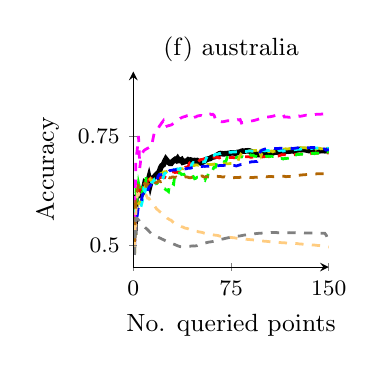
\begin{tikzpicture}

% defining custom colors
\definecolor{mycolor1}{rgb}{0.8,0.8,0}
\definecolor{mycolor2}{rgb}{0,1,1}
\definecolor{mycolor3}{rgb}{1,0,1}
\definecolor{mycolor4}{rgb}{1,0.8,0.5}
\definecolor{mycolor5}{rgb}{0.7,0.4,0.01}


\begin{axis}[
footnotesize,
width= 1.6in,
height= 1.6in,
xmin=0, xmax=150,
ymin=0.45, ymax=0.9,
xlabel = {No. queried points},
ylabel = {Accuracy},
title={(f) australia},
ytick={0.5,0.75},
xtick = {0,75,150},
axis on top,
axis y line = left,
axis x line = bottom
%legend entries={$optimal$,$rand$,$IVM$,$maxent$,$QBC2$,$QBC100$,$SVM$},
 %egend style={nodes=right}
]
\addplot [
color=black,
solid,
line width=2.0pt
]
coordinates{ (1,0.524294) (2,0.610656) (3,0.613715) (4,0.617174) (5,0.621455) (6,0.615766) (7,0.621553) (8,0.630634) (9,0.644258) (10,0.642385) (11,0.643743) (12,0.654769) (13,0.641156) (14,0.653375) (15,0.654953) (16,0.656878) (17,0.660488) (18,0.663482) (19,0.659406) (20,0.669725) (21,0.678924) (22,0.68377) (23,0.685407) (24,0.692433) (25,0.698311) (26,0.694533) (27,0.691337) (28,0.688778) (29,0.688643) (30,0.692574) (31,0.695293) (32,0.697498) (33,0.695482) (34,0.699647) (35,0.694968) (36,0.695079) (37,0.696948) (38,0.691309) (39,0.692124) (40,0.69389) (41,0.693957) (42,0.69655) (43,0.694349) (44,0.696393) (45,0.695488) (46,0.69406) (47,0.695331) (48,0.694224) (49,0.695185) (50,0.693271) (51,0.690752) (52,0.689555) (53,0.691524) (54,0.69288) (55,0.69454) (56,0.69741) (57,0.698311) (58,0.699245) (59,0.699938) (60,0.702158) (61,0.703238) (62,0.703861) (63,0.704752) (64,0.706863) (65,0.708771) (66,0.710714) (67,0.711376) (68,0.711043) (69,0.710749) (70,0.710797) (71,0.711325) (72,0.711214) (73,0.711612) (74,0.71181) (75,0.712923) (76,0.71306) (77,0.712805) (78,0.712076) (79,0.712594) (80,0.714029) (81,0.714248) (82,0.715054) (83,0.716421) (84,0.717125) (85,0.716979) (86,0.717118) (87,0.717596) (88,0.717755) (89,0.717484) (90,0.71621) (91,0.715278) (92,0.713003) (93,0.712493) (94,0.709409) (95,0.709132) (96,0.708926) (97,0.70887) (98,0.708838) (99,0.709064) (100,0.710362) (101,0.710774) (102,0.710824) (103,0.710457) (104,0.710406) (105,0.710756) (106,0.711544) (107,0.713048) (108,0.71398) (109,0.71458) (110,0.714509) (111,0.714773) (112,0.715306) (113,0.715287) (114,0.714675) (115,0.71461) (116,0.715422) (117,0.716426) (118,0.716782) (119,0.716645) (120,0.717028) (121,0.717304) (122,0.717473) (123,0.717123) (124,0.717837) (125,0.718772) (126,0.719788) (127,0.720221) (128,0.720821) (129,0.720409) (130,0.720519) (131,0.720224) (132,0.719992) (133,0.719335) (134,0.718531) (135,0.718072) (136,0.717813) (137,0.717894) (138,0.718041) (139,0.717537) (140,0.717571) (141,0.717637) (142,0.717671) (143,0.717674) (144,0.717937) (145,0.718194) (146,0.717946) (147,0.717709) (148,0.718095) (149,0.719119) (150,0.719025)
};

\addplot [
color=red,
dashed,
line width=1.0pt
]
coordinates{ (1,0.510636) (2,0.611135) (3,0.608563) (4,0.618412) (5,0.627911) (6,0.631634) (7,0.635265) (8,0.63776) (9,0.635813) (10,0.644056) (11,0.649147) (12,0.651703) (13,0.64956) (14,0.657673) (15,0.65461) (16,0.654381) (17,0.655276) (18,0.653187) (19,0.654352) (20,0.655241) (21,0.656221) (22,0.657321) (23,0.656154) (24,0.655918) (25,0.6625) (26,0.663072) (27,0.666502) (28,0.667788) (29,0.667238) (30,0.668626) (31,0.669417) (32,0.66777) (33,0.668401) (34,0.667696) (35,0.668321) (36,0.673093) (37,0.672971) (38,0.672851) (39,0.673219) (40,0.679665) (41,0.680388) (42,0.680014) (43,0.689139) (44,0.691667) (45,0.69273) (46,0.692195) (47,0.692765) (48,0.692563) (49,0.692651) (50,0.692619) (51,0.696084) (52,0.697568) (53,0.697299) (54,0.698988) (55,0.698594) (56,0.698489) (57,0.698611) (58,0.698685) (59,0.704089) (60,0.70379) (61,0.703383) (62,0.7028) (63,0.703104) (64,0.702462) (65,0.702187) (66,0.701045) (67,0.702327) (68,0.702779) (69,0.702489) (70,0.702653) (71,0.702058) (72,0.702488) (73,0.702389) (74,0.702355) (75,0.702303) (76,0.702456) (77,0.701784) (78,0.701844) (79,0.701994) (80,0.701532) (81,0.701488) (82,0.701636) (83,0.702078) (84,0.701602) (85,0.703766) (86,0.703939) (87,0.703736) (88,0.704123) (89,0.703739) (90,0.702735) (91,0.702963) (92,0.703297) (93,0.702587) (94,0.702311) (95,0.704124) (96,0.703553) (97,0.703424) (98,0.704005) (99,0.703502) (100,0.703961) (101,0.7043) (102,0.704237) (103,0.704608) (104,0.703789) (105,0.703872) (106,0.704223) (107,0.704034) (108,0.7046) (109,0.705518) (110,0.70524) (111,0.705401) (112,0.706474) (113,0.707452) (114,0.70884) (115,0.708628) (116,0.708662) (117,0.708036) (118,0.707957) (119,0.709137) (120,0.708816) (121,0.708473) (122,0.708255) (123,0.708077) (124,0.708994) (125,0.709782) (126,0.710105) (127,0.70979) (128,0.709903) (129,0.710378) (130,0.710809) (131,0.711564) (132,0.711149) (133,0.711135) (134,0.711168) (135,0.710465) (136,0.711033) (137,0.711364) (138,0.712151) (139,0.71178) (140,0.712105) (141,0.712113) (142,0.712874) (143,0.71321) (144,0.713222) (145,0.713463) (146,0.713391) (147,0.713306) (148,0.713176) (149,0.712881) (150,0.712572)
};

\addplot [
color=green,
dashed,
line width=1.0pt
]
coordinates{ (1,0.543747) (2,0.622537) (3,0.612673) (4,0.6439) (5,0.630728) (6,0.636914) (7,0.620869) (8,0.642724) (9,0.634601) (10,0.65904) (11,0.65324) (12,0.653581) (13,0.650485) (14,0.650427) (15,0.649823) (16,0.648982) (17,0.644392) (18,0.643622) (19,0.639782) (20,0.638638) (21,0.633596) (22,0.632431) (23,0.63139) (24,0.630699) (25,0.627736) (26,0.626516) (27,0.62387) (28,0.643891) (29,0.641795) (30,0.642423) (31,0.640688) (32,0.667836) (33,0.667077) (34,0.6674) (35,0.666501) (36,0.666704) (37,0.663) (38,0.663784) (39,0.662894) (40,0.664365) (41,0.665104) (42,0.665608) (43,0.664173) (44,0.664609) (45,0.657361) (46,0.65835) (47,0.653376) (48,0.654393) (49,0.656957) (50,0.6572) (51,0.656046) (52,0.656071) (53,0.652172) (54,0.652409) (55,0.650035) (56,0.65827) (57,0.657838) (58,0.673005) (59,0.67318) (60,0.675891) (61,0.673934) (62,0.68) (63,0.679829) (64,0.689164) (65,0.688453) (66,0.688879) (67,0.687343) (68,0.68773) (69,0.68686) (70,0.692979) (71,0.692925) (72,0.702027) (73,0.70089) (74,0.703891) (75,0.701094) (76,0.703121) (77,0.702334) (78,0.702602) (79,0.701996) (80,0.703222) (81,0.702975) (82,0.704706) (83,0.703525) (84,0.703882) (85,0.702161) (86,0.70731) (87,0.706018) (88,0.706368) (89,0.705759) (90,0.708218) (91,0.707144) (92,0.707718) (93,0.705038) (94,0.704982) (95,0.704258) (96,0.70458) (97,0.704309) (98,0.704561) (99,0.704553) (100,0.704749) (101,0.704116) (102,0.704867) (103,0.704755) (104,0.705343) (105,0.704654) (106,0.704974) (107,0.704719) (108,0.704838) (109,0.703397) (110,0.70345) (111,0.703114) (112,0.703524) (113,0.699672) (114,0.70012) (115,0.6987) (116,0.700045) (117,0.699633) (118,0.700318) (119,0.700483) (120,0.700712) (121,0.700439) (122,0.705844) (123,0.705634) (124,0.708505) (125,0.708127) (126,0.710062) (127,0.709094) (128,0.710098) (129,0.709831) (130,0.709951) (131,0.709612) (132,0.711419) (133,0.711281) (134,0.711612) (135,0.710917) (136,0.711143) (137,0.711593) (138,0.711848) (139,0.710908) (140,0.712771) (141,0.711923) (142,0.712115) (143,0.711993) (144,0.71479) (145,0.714067) (146,0.714982) (147,0.714527) (148,0.714812) (149,0.714557) (150,0.714765)
};

\addplot [
color=mycolor1,
dashed,
line width=1.0pt
]
coordinates{ (1,0.480981) (2,0.582793) (3,0.594817) (4,0.595591) (5,0.599427) (6,0.601578) (7,0.621437) (8,0.621127) (9,0.636069) (10,0.630923) (11,0.63399) (12,0.648314) (13,0.652397) (14,0.645693) (15,0.648646) (16,0.654734) (17,0.656969) (18,0.657527) (19,0.661438) (20,0.663508) (21,0.664885) (22,0.665755) (23,0.668473) (24,0.669343) (25,0.669274) (26,0.670374) (27,0.671501) (28,0.67212) (29,0.672576) (30,0.674279) (31,0.675008) (32,0.674584) (33,0.675035) (34,0.674911) (35,0.675145) (36,0.674808) (37,0.676172) (38,0.676242) (39,0.677233) (40,0.677072) (41,0.677488) (42,0.677715) (43,0.677608) (44,0.678587) (45,0.684095) (46,0.684011) (47,0.684032) (48,0.685187) (49,0.684939) (50,0.684262) (51,0.685126) (52,0.684609) (53,0.685416) (54,0.685612) (55,0.68606) (56,0.686279) (57,0.686403) (58,0.686093) (59,0.68622) (60,0.686128) (61,0.686594) (62,0.686979) (63,0.68693) (64,0.687045) (65,0.687275) (66,0.687338) (67,0.687473) (68,0.687257) (69,0.687631) (70,0.687659) (71,0.687861) (72,0.68778) (73,0.687874) (74,0.688156) (75,0.688309) (76,0.688316) (77,0.688317) (78,0.6885) (79,0.688969) (80,0.690457) (81,0.700069) (82,0.7067) (83,0.712086) (84,0.715426) (85,0.716857) (86,0.715272) (87,0.716261) (88,0.717251) (89,0.717913) (90,0.717988) (91,0.717732) (92,0.71778) (93,0.718279) (94,0.71822) (95,0.705439) (96,0.711939) (97,0.715758) (98,0.706335) (99,0.712976) (100,0.708555) (101,0.712653) (102,0.71341) (103,0.716133) (104,0.715589) (105,0.716787) (106,0.716974) (107,0.715252) (108,0.717061) (109,0.716719) (110,0.717174) (111,0.717679) (112,0.719736) (113,0.719743) (114,0.720274) (115,0.721119) (116,0.721768) (117,0.722264) (118,0.721786) (119,0.722183) (120,0.722704) (121,0.72241) (122,0.722524) (123,0.72302) (124,0.723779) (125,0.723868) (126,0.724004) (127,0.724318) (128,0.724377) (129,0.724478) (130,0.72473) (131,0.724879) (132,0.724789) (133,0.723801) (134,0.72418) (135,0.723503) (136,0.722007) (137,0.721327) (138,0.717731) (139,0.720274) (140,0.721439) (141,0.722478) (142,0.723562) (143,0.723459) (144,0.722114) (145,0.722333) (146,0.723701) (147,0.724347) (148,0.724195) (149,0.724141) (150,0.724787)
};

\addplot [
color=mycolor2,
dashed,
line width=1.0pt
]
coordinates{ (1,0.525887) (2,0.595505) (3,0.571379) (4,0.579594) (5,0.580516) (6,0.590079) (7,0.601837) (8,0.628332) (9,0.623922) (10,0.629891) (11,0.633731) (12,0.63038) (13,0.632366) (14,0.644084) (15,0.645717) (16,0.650583) (17,0.644485) (18,0.649928) (19,0.65407) (20,0.657314) (21,0.658537) (22,0.657584) (23,0.655783) (24,0.665258) (25,0.667256) (26,0.671289) (27,0.670938) (28,0.672022) (29,0.67184) (30,0.672958) (31,0.674374) (32,0.674938) (33,0.674562) (34,0.676033) (35,0.675217) (36,0.677091) (37,0.677515) (38,0.678419) (39,0.677912) (40,0.677066) (41,0.676506) (42,0.677872) (43,0.678222) (44,0.678144) (45,0.68739) (46,0.690751) (47,0.690028) (48,0.690006) (49,0.690356) (50,0.690719) (51,0.691469) (52,0.692554) (53,0.691772) (54,0.692323) (55,0.692152) (56,0.700647) (57,0.706404) (58,0.706215) (59,0.703776) (60,0.704765) (61,0.70901) (62,0.707178) (63,0.709589) (64,0.709492) (65,0.710031) (66,0.71146) (67,0.710928) (68,0.712607) (69,0.713299) (70,0.714721) (71,0.715469) (72,0.715702) (73,0.714464) (74,0.714326) (75,0.714024) (76,0.714874) (77,0.714799) (78,0.714742) (79,0.715142) (80,0.715457) (81,0.715005) (82,0.715202) (83,0.715927) (84,0.715321) (85,0.716068) (86,0.715873) (87,0.716289) (88,0.716669) (89,0.717329) (90,0.71713) (91,0.716796) (92,0.716453) (93,0.716338) (94,0.717224) (95,0.716964) (96,0.716585) (97,0.716488) (98,0.717026) (99,0.717658) (100,0.717763) (101,0.717373) (102,0.718078) (103,0.718354) (104,0.718222) (105,0.719179) (106,0.719196) (107,0.719227) (108,0.719459) (109,0.719055) (110,0.719136) (111,0.720119) (112,0.718163) (113,0.718645) (114,0.719068) (115,0.716952) (116,0.717555) (117,0.718007) (118,0.718105) (119,0.718798) (120,0.718663) (121,0.719473) (122,0.720025) (123,0.720047) (124,0.720354) (125,0.720554) (126,0.721137) (127,0.721253) (128,0.721444) (129,0.721544) (130,0.722111) (131,0.721922) (132,0.721916) (133,0.722716) (134,0.722043) (135,0.722509) (136,0.723055) (137,0.722982) (138,0.72422) (139,0.724175) (140,0.72404) (141,0.723897) (142,0.723659) (143,0.723778) (144,0.723556) (145,0.723161) (146,0.723533) (147,0.723499) (148,0.723659) (149,0.723594) (150,0.72376)
};

\addplot [
color=blue,
dashed,
line width=1.0pt
]
coordinates{ (1,0.494938) (2,0.570079) (3,0.568943) (4,0.590613) (5,0.595701) (6,0.598402) (7,0.616559) (8,0.61938) (9,0.621263) (10,0.628922) (11,0.623312) (12,0.634492) (13,0.636994) (14,0.642193) (15,0.644035) (16,0.647851) (17,0.647062) (18,0.647766) (19,0.659289) (20,0.662985) (21,0.662304) (22,0.66364) (23,0.663929) (24,0.664927) (25,0.668987) (26,0.670042) (27,0.668838) (28,0.672053) (29,0.672582) (30,0.672914) (31,0.673864) (32,0.672972) (33,0.674559) (34,0.674447) (35,0.674557) (36,0.675326) (37,0.673765) (38,0.674002) (39,0.675734) (40,0.676048) (41,0.67654) (42,0.677593) (43,0.677684) (44,0.677794) (45,0.678719) (46,0.679161) (47,0.679417) (48,0.679346) (49,0.679958) (50,0.680749) (51,0.681227) (52,0.681499) (53,0.681692) (54,0.681898) (55,0.681714) (56,0.68197) (57,0.681818) (58,0.681934) (59,0.682304) (60,0.682602) (61,0.682705) (62,0.682929) (63,0.682909) (64,0.683356) (65,0.683306) (66,0.683576) (67,0.683728) (68,0.683688) (69,0.683863) (70,0.684237) (71,0.684343) (72,0.684444) (73,0.684403) (74,0.681831) (75,0.68312) (76,0.683647) (77,0.683731) (78,0.683485) (79,0.682587) (80,0.683713) (81,0.684401) (82,0.685607) (83,0.686008) (84,0.688726) (85,0.688746) (86,0.690253) (87,0.690304) (88,0.690707) (89,0.691051) (90,0.691851) (91,0.692312) (92,0.692343) (93,0.692695) (94,0.693163) (95,0.693031) (96,0.702659) (97,0.712614) (98,0.717792) (99,0.719493) (100,0.72083) (101,0.721692) (102,0.722112) (103,0.722064) (104,0.722068) (105,0.721898) (106,0.722875) (107,0.723232) (108,0.722536) (109,0.722806) (110,0.723041) (111,0.723053) (112,0.723224) (113,0.723279) (114,0.723447) (115,0.723519) (116,0.723743) (117,0.723799) (118,0.722912) (119,0.723144) (120,0.72367) (121,0.723701) (122,0.722386) (123,0.723128) (124,0.723484) (125,0.723949) (126,0.724462) (127,0.724783) (128,0.724987) (129,0.724349) (130,0.7247) (131,0.724215) (132,0.724026) (133,0.724497) (134,0.724806) (135,0.724629) (136,0.724984) (137,0.725091) (138,0.725196) (139,0.7252) (140,0.725371) (141,0.725308) (142,0.724922) (143,0.723241) (144,0.722643) (145,0.721707) (146,0.721837) (147,0.721452) (148,0.719054) (149,0.71985) (150,0.71981)
};

\addplot [
color=mycolor3,
dashed,
line width=1.0pt
]
coordinates{ (1,0.555998) (2,0.696341) (3,0.71959) (4,0.751873) (5,0.67829) (6,0.704935) (7,0.712585) (8,0.717739) (9,0.720039) (10,0.721833) (11,0.72346) (12,0.725003) (13,0.731013) (14,0.729313) (15,0.743107) (16,0.758318) (17,0.75886) (18,0.766026) (19,0.768374) (20,0.774107) (21,0.778242) (22,0.78265) (23,0.786398) (24,0.770873) (25,0.773081) (26,0.774442) (27,0.775501) (28,0.77617) (29,0.776977) (30,0.778923) (31,0.78114) (32,0.783253) (33,0.784722) (34,0.787247) (35,0.790044) (36,0.792187) (37,0.793923) (38,0.795167) (39,0.796159) (40,0.796694) (41,0.798209) (42,0.798568) (43,0.799121) (44,0.799335) (45,0.800306) (46,0.79366) (47,0.79498) (48,0.795609) (49,0.797442) (50,0.798178) (51,0.798644) (52,0.799033) (53,0.797624) (54,0.797514) (55,0.800107) (56,0.801214) (57,0.801487) (58,0.802453) (59,0.802511) (60,0.800954) (61,0.801749) (62,0.799134) (63,0.790474) (64,0.791717) (65,0.791255) (66,0.785021) (67,0.785168) (68,0.78437) (69,0.784712) (70,0.785114) (71,0.785946) (72,0.786536) (73,0.786733) (74,0.786793) (75,0.786575) (76,0.786865) (77,0.787362) (78,0.788448) (79,0.788381) (80,0.789389) (81,0.788732) (82,0.789527) (83,0.781574) (84,0.782584) (85,0.782662) (86,0.783287) (87,0.783947) (88,0.783838) (89,0.784771) (90,0.785785) (91,0.786452) (92,0.787021) (93,0.787752) (94,0.788552) (95,0.789383) (96,0.790533) (97,0.791619) (98,0.792197) (99,0.792807) (100,0.79381) (101,0.794659) (102,0.79496) (103,0.795281) (104,0.795733) (105,0.796033) (106,0.796704) (107,0.797216) (108,0.798163) (109,0.798889) (110,0.799502) (111,0.799916) (112,0.799681) (113,0.799986) (114,0.800292) (115,0.800657) (116,0.795301) (117,0.795596) (118,0.79528) (119,0.795071) (120,0.794714) (121,0.795547) (122,0.796271) (123,0.796657) (124,0.797097) (125,0.79766) (126,0.796999) (127,0.79782) (128,0.796929) (129,0.797532) (130,0.797989) (131,0.798704) (132,0.799316) (133,0.799614) (134,0.799121) (135,0.799152) (136,0.799347) (137,0.79996) (138,0.800478) (139,0.800899) (140,0.801435) (141,0.801754) (142,0.801713) (143,0.80181) (144,0.801969) (145,0.802291) (146,0.802533) (147,0.802409) (148,0.802485) (149,0.802392) (150,0.802414)
};

\addplot [
color=mycolor4,
dashed,
line width=1.0pt
]
coordinates{ (1,0.493515) (2,0.575597) (3,0.618004) (4,0.616438) (5,0.624953) (6,0.623173) (7,0.619634) (8,0.617444) (9,0.618066) (10,0.614788) (11,0.608307) (12,0.60845) (13,0.602741) (14,0.601466) (15,0.597986) (16,0.591629) (17,0.587709) (18,0.583351) (19,0.581136) (20,0.578262) (21,0.576006) (22,0.573862) (23,0.572061) (24,0.568044) (25,0.565423) (26,0.562539) (27,0.560946) (28,0.558797) (29,0.557858) (30,0.554762) (31,0.552083) (32,0.549674) (33,0.548225) (34,0.547142) (35,0.545935) (36,0.544468) (37,0.542897) (38,0.542169) (39,0.540712) (40,0.539339) (41,0.538979) (42,0.538184) (43,0.536672) (44,0.53626) (45,0.535686) (46,0.534406) (47,0.53352) (48,0.532554) (49,0.532183) (50,0.531149) (51,0.530672) (52,0.530195) (53,0.529651) (54,0.528382) (55,0.527594) (56,0.527213) (57,0.526518) (58,0.526234) (59,0.525657) (60,0.524714) (61,0.524275) (62,0.523749) (63,0.523421) (64,0.523023) (65,0.522687) (66,0.521411) (67,0.520765) (68,0.520394) (69,0.520076) (70,0.519765) (71,0.519416) (72,0.519052) (73,0.518783) (74,0.518455) (75,0.518102) (76,0.517762) (77,0.517444) (78,0.517125) (79,0.516538) (80,0.516294) (81,0.515963) (82,0.515637) (83,0.515338) (84,0.515038) (85,0.514792) (86,0.514446) (87,0.513861) (88,0.513629) (89,0.513295) (90,0.513018) (91,0.512744) (92,0.512538) (93,0.512294) (94,0.512036) (95,0.511746) (96,0.511438) (97,0.511043) (98,0.510227) (99,0.509979) (100,0.509717) (101,0.509532) (102,0.509282) (103,0.508829) (104,0.508591) (105,0.508127) (106,0.50791) (107,0.507656) (108,0.507427) (109,0.507238) (110,0.507055) (111,0.506587) (112,0.506455) (113,0.506305) (114,0.506106) (115,0.505898) (116,0.505759) (117,0.505575) (118,0.505298) (119,0.505175) (120,0.505016) (121,0.504869) (122,0.504583) (123,0.50439) (124,0.504238) (125,0.504023) (126,0.50393) (127,0.503402) (128,0.503236) (129,0.503008) (130,0.502607) (131,0.502267) (132,0.502083) (133,0.501921) (134,0.501769) (135,0.501588) (136,0.501411) (137,0.500966) (138,0.500823) (139,0.500621) (140,0.500296) (141,0.499896) (142,0.499643) (143,0.499407) (144,0.498996) (145,0.498508) (146,0.498255) (147,0.497695) (148,0.497445) (149,0.496728) (150,0.496219)
};

\addplot [
color=mycolor5,
dashed,
line width=1.0pt
]
coordinates{ (1,0.508263) (2,0.620698) (3,0.625502) (4,0.640004) (5,0.6428) (6,0.649255) (7,0.647832) (8,0.642954) (9,0.643049) (10,0.636915) (11,0.640644) (12,0.644329) (13,0.640346) (14,0.644751) (15,0.644301) (16,0.646784) (17,0.643621) (18,0.644473) (19,0.647165) (20,0.648355) (21,0.646412) (22,0.647304) (23,0.648123) (24,0.650327) (25,0.653216) (26,0.655026) (27,0.656365) (28,0.655344) (29,0.655853) (30,0.65739) (31,0.657077) (32,0.656665) (33,0.657129) (34,0.655285) (35,0.656534) (36,0.656016) (37,0.655843) (38,0.656079) (39,0.656863) (40,0.657718) (41,0.657398) (42,0.656728) (43,0.655553) (44,0.655641) (45,0.656585) (46,0.657149) (47,0.65706) (48,0.657903) (49,0.657906) (50,0.658631) (51,0.659241) (52,0.659633) (53,0.659782) (54,0.657493) (55,0.657445) (56,0.657788) (57,0.65784) (58,0.65769) (59,0.657459) (60,0.657772) (61,0.657085) (62,0.658068) (63,0.658792) (64,0.658892) (65,0.658727) (66,0.658688) (67,0.658357) (68,0.657526) (69,0.657249) (70,0.657899) (71,0.656452) (72,0.655723) (73,0.655178) (74,0.654549) (75,0.65449) (76,0.655365) (77,0.655518) (78,0.656213) (79,0.65624) (80,0.655918) (81,0.656074) (82,0.656707) (83,0.657253) (84,0.657263) (85,0.656948) (86,0.657285) (87,0.657155) (88,0.656412) (89,0.656504) (90,0.656132) (91,0.656262) (92,0.655752) (93,0.656655) (94,0.656496) (95,0.656921) (96,0.657118) (97,0.657681) (98,0.658071) (99,0.658064) (100,0.657712) (101,0.658453) (102,0.65768) (103,0.658034) (104,0.658485) (105,0.658627) (106,0.658527) (107,0.658101) (108,0.658194) (109,0.65847) (110,0.658663) (111,0.659168) (112,0.659257) (113,0.659427) (114,0.659199) (115,0.659103) (116,0.658931) (117,0.658026) (118,0.658333) (119,0.658445) (120,0.658489) (121,0.658226) (122,0.658306) (123,0.659199) (124,0.659739) (125,0.660473) (126,0.661005) (127,0.661382) (128,0.661635) (129,0.661871) (130,0.662244) (131,0.662546) (132,0.662708) (133,0.662998) (134,0.663319) (135,0.6633) (136,0.663661) (137,0.664033) (138,0.664218) (139,0.664367) (140,0.664283) (141,0.664728) (142,0.664737) (143,0.664635) (144,0.664677) (145,0.664811) (146,0.664622) (147,0.664602) (148,0.664776) (149,0.664909) (150,0.664884)
};

\addplot [
color=gray,
dashed,
line width=1.0pt
]
coordinates{ (1,0.47782) (2,0.562155) (3,0.561781) (4,0.558965) (5,0.55469) (6,0.550887) (7,0.547557) (8,0.544243) (9,0.5412) (10,0.538685) (11,0.535914) (12,0.532679) (13,0.529607) (14,0.526671) (15,0.525895) (16,0.523843) (17,0.521994) (18,0.520213) (19,0.518684) (20,0.517306) (21,0.516071) (22,0.514439) (23,0.513087) (24,0.511573) (25,0.510257) (26,0.508923) (27,0.507709) (28,0.506279) (29,0.505112) (30,0.504082) (31,0.502746) (32,0.501628) (33,0.500311) (34,0.499043) (35,0.497981) (36,0.497107) (37,0.496846) (38,0.496438) (39,0.496762) (40,0.497114) (41,0.497745) (42,0.497971) (43,0.498004) (44,0.498137) (45,0.498601) (46,0.498775) (47,0.498495) (48,0.498867) (49,0.499297) (50,0.500674) (51,0.5017) (52,0.502423) (53,0.50322) (54,0.504351) (55,0.505288) (56,0.506079) (57,0.506786) (58,0.507494) (59,0.507867) (60,0.508403) (61,0.508764) (62,0.509314) (63,0.509961) (64,0.511057) (65,0.511639) (66,0.512571) (67,0.513613) (68,0.514266) (69,0.514815) (70,0.515516) (71,0.516264) (72,0.516933) (73,0.517523) (74,0.5182) (75,0.518808) (76,0.519351) (77,0.519849) (78,0.520253) (79,0.520332) (80,0.521033) (81,0.521325) (82,0.521712) (83,0.522318) (84,0.522919) (85,0.523529) (86,0.523846) (87,0.5241) (88,0.524339) (89,0.525001) (90,0.525287) (91,0.525677) (92,0.52614) (93,0.526496) (94,0.526999) (95,0.527282) (96,0.527608) (97,0.527827) (98,0.527932) (99,0.528222) (100,0.528373) (101,0.52842) (102,0.528607) (103,0.528784) (104,0.528957) (105,0.529196) (106,0.529413) (107,0.529498) (108,0.529392) (109,0.529419) (110,0.529297) (111,0.529193) (112,0.529135) (113,0.529176) (114,0.529246) (115,0.529268) (116,0.529284) (117,0.529355) (118,0.529257) (119,0.529163) (120,0.529247) (121,0.529211) (122,0.52908) (123,0.529096) (124,0.529164) (125,0.52903) (126,0.528957) (127,0.528767) (128,0.528623) (129,0.528549) (130,0.528518) (131,0.52839) (132,0.528316) (133,0.528258) (134,0.528288) (135,0.528409) (136,0.528416) (137,0.528465) (138,0.528395) (139,0.52822) (140,0.528075) (141,0.528016) (142,0.527836) (143,0.527799) (144,0.52772) (145,0.527752) (146,0.527653) (147,0.527576) (148,0.523584) (149,0.517122) (150,0.511372)
};

\end{axis}
\end{tikzpicture}
\\
% This file was created by matlab2tikz v0.0.7.
% Copyright (c) 2008--2010, Nico Schlömer <nico.schloemer@gmail.com>
% All rights reserved.
% 
% The latest updates can be retrieved from
%   http://www.mathworks.com/matlabcentral/fileexchange/22022-matlab2tikz
% where you can also make suggestions and rate matlab2tikz.
% 
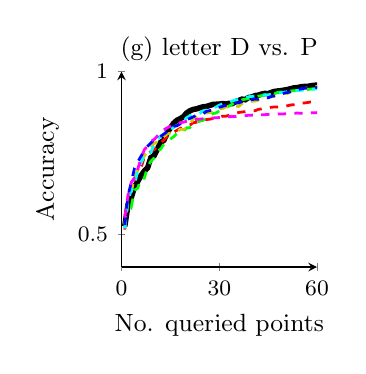
\begin{tikzpicture}

% defining custom colors
\definecolor{mycolor1}{rgb}{0.8,0.8,0}
\definecolor{mycolor2}{rgb}{0,1,1}
\definecolor{mycolor3}{rgb}{1,0,1}


\begin{axis}[
footnotesize,
width= 1.6in,
height= 1.6in,
xmin=0, xmax=60,
ymin=0.4, ymax=1,
title={(g) letter D vs. P},
xlabel = {No. queried points},
ylabel = {Accuracy},
ytick={0.5,1},
xtick = {0,30,60},
axis on top,
axis y line = left,
axis x line = bottom
%legend entries={$optimal$,$rand$,$IVM$,$maxent$,$QBC2$,$QBC100$,$SVM$},
 %egend style={nodes=right}
]
\addplot [
color=black,
solid,
line width=2.0pt
]
coordinates{ (1,0.525525) (2,0.591883) (3,0.613674) (4,0.646068) (5,0.663602) (6,0.680721) (7,0.694746) (8,0.704622) (9,0.735791) (10,0.742039) (11,0.761652) (12,0.78265) (13,0.789146) (14,0.811389) (15,0.827244) (16,0.841445) (17,0.850241) (18,0.85526) (19,0.861531) (20,0.873021) (21,0.879598) (22,0.883694) (23,0.885579) (24,0.888944) (25,0.891639) (26,0.892832) (27,0.895951) (28,0.898932) (29,0.899677) (30,0.900171) (31,0.90162) (32,0.900091) (33,0.902351) (34,0.901725) (35,0.9075) (36,0.91132) (37,0.915415) (38,0.913755) (39,0.920406) (40,0.921845) (41,0.926337) (42,0.927662) (43,0.930857) (44,0.932976) (45,0.931937) (46,0.936099) (47,0.93912) (48,0.940473) (49,0.941432) (50,0.943348) (51,0.944911) (52,0.94766) (53,0.950104) (54,0.950643) (55,0.953257) (56,0.954223) (57,0.954116) (58,0.956215) (59,0.957767) (60,0.958319) (61,0.959119) (62,0.960128) (63,0.961483) (64,0.962489) (65,0.962832) (66,0.963738) (67,0.964199) (68,0.965043) (69,0.965777) (70,0.966498) (71,0.967) (72,0.967667) (73,0.96823) (74,0.968841) (75,0.969499) (76,0.969898) (77,0.970466) (78,0.97093) (79,0.971249) (80,0.971657) (81,0.971955) (82,0.972276) (83,0.972673) (84,0.973099) (85,0.973444) (86,0.97372) (87,0.973895) (88,0.97416) (89,0.974582) (90,0.974913) (91,0.97511) (92,0.975361) (93,0.975538) (94,0.975739) (95,0.975917) (96,0.976141) (97,0.976349) (98,0.976562) (99,0.976795) (100,0.976946)
};

\addplot [
color=red,
dashed,
line width=1.0pt
]
coordinates{ (1,0.514899) (2,0.617224) (3,0.647191) (4,0.668673) (5,0.690986) (6,0.704808) (7,0.737915) (8,0.743407) (9,0.754848) (10,0.760296) (11,0.769142) (12,0.782479) (13,0.789654) (14,0.800925) (15,0.808251) (16,0.814113) (17,0.819727) (18,0.825418) (19,0.830743) (20,0.833991) (21,0.835856) (22,0.843019) (23,0.844389) (24,0.847693) (25,0.85084) (26,0.852467) (27,0.853767) (28,0.855424) (29,0.857562) (30,0.859409) (31,0.862967) (32,0.862838) (33,0.865774) (34,0.871841) (35,0.872526) (36,0.874507) (37,0.875842) (38,0.877144) (39,0.878819) (40,0.878943) (41,0.879985) (42,0.883981) (43,0.885609) (44,0.888037) (45,0.888863) (46,0.890644) (47,0.891236) (48,0.891467) (49,0.892335) (50,0.893669) (51,0.895276) (52,0.897581) (53,0.898501) (54,0.899393) (55,0.90285) (56,0.903488) (57,0.90493) (58,0.906669) (59,0.906216) (60,0.909271) (61,0.909933) (62,0.9106) (63,0.910912) (64,0.91351) (65,0.913873) (66,0.914437) (67,0.915139) (68,0.916078) (69,0.916376) (70,0.916949) (71,0.91719) (72,0.917521) (73,0.920672) (74,0.921025) (75,0.921736) (76,0.923296) (77,0.92423) (78,0.924371) (79,0.924777) (80,0.925354) (81,0.925312) (82,0.925816) (83,0.926928) (84,0.92715) (85,0.927415) (86,0.927804) (87,0.928802) (88,0.929226) (89,0.92949) (90,0.929835) (91,0.930795) (92,0.931844) (93,0.932039) (94,0.932385) (95,0.932316) (96,0.932442) (97,0.932677) (98,0.93277) (99,0.932969) (100,0.933123)
};

\addplot [
color=green,
dashed,
line width=1.0pt
]
coordinates{ (1,0.521542) (2,0.602944) (3,0.585381) (4,0.636286) (5,0.642073) (6,0.673147) (7,0.672784) (8,0.707634) (9,0.724604) (10,0.734918) (11,0.755777) (12,0.761775) (13,0.776843) (14,0.783744) (15,0.792627) (16,0.800257) (17,0.810164) (18,0.814645) (19,0.816444) (20,0.827267) (21,0.828167) (22,0.839008) (23,0.844205) (24,0.847828) (25,0.850246) (26,0.860574) (27,0.864353) (28,0.87065) (29,0.872869) (30,0.879195) (31,0.882358) (32,0.889972) (33,0.894399) (34,0.900162) (35,0.905765) (36,0.909576) (37,0.913459) (38,0.915382) (39,0.917199) (40,0.919361) (41,0.921757) (42,0.924584) (43,0.926022) (44,0.928915) (45,0.930048) (46,0.93151) (47,0.93239) (48,0.936179) (49,0.937142) (50,0.938346) (51,0.939322) (52,0.94051) (53,0.941331) (54,0.94192) (55,0.942422) (56,0.943821) (57,0.944851) (58,0.946276) (59,0.946683) (60,0.947413) (61,0.947889) (62,0.948622) (63,0.948956) (64,0.950848) (65,0.951013) (66,0.952123) (67,0.952536) (68,0.95299) (69,0.953208) (70,0.95436) (71,0.95482) (72,0.9554) (73,0.95583) (74,0.956294) (75,0.956656) (76,0.956984) (77,0.957792) (78,0.958064) (79,0.958455) (80,0.958585) (81,0.958987) (82,0.959274) (83,0.959696) (84,0.959924) (85,0.960747) (86,0.960956) (87,0.96106) (88,0.961344) (89,0.961653) (90,0.962055) (91,0.96218) (92,0.962485) (93,0.962779) (94,0.962998) (95,0.963291) (96,0.963596) (97,0.963754) (98,0.964031) (99,0.964168) (100,0.964373)
};

\addplot [
color=mycolor1,
dashed,
line width=1.0pt
]
coordinates{ (1,0.530829) (2,0.610573) (3,0.630616) (4,0.674898) (5,0.697094) (6,0.720098) (7,0.74044) (8,0.757952) (9,0.768414) (10,0.779247) (11,0.78477) (12,0.788056) (13,0.800888) (14,0.808052) (15,0.81148) (16,0.81178) (17,0.814812) (18,0.8228) (19,0.822388) (20,0.826042) (21,0.839726) (22,0.854303) (23,0.859846) (24,0.867218) (25,0.871924) (26,0.872589) (27,0.873701) (28,0.881378) (29,0.884862) (30,0.885311) (31,0.886811) (32,0.891039) (33,0.892525) (34,0.894432) (35,0.893907) (36,0.892877) (37,0.902133) (38,0.903094) (39,0.907839) (40,0.908282) (41,0.909717) (42,0.912389) (43,0.914861) (44,0.91773) (45,0.920408) (46,0.922583) (47,0.924884) (48,0.927102) (49,0.931141) (50,0.93363) (51,0.933074) (52,0.937924) (53,0.940598) (54,0.943333) (55,0.945579) (56,0.947787) (57,0.950402) (58,0.951737) (59,0.953032) (60,0.954464) (61,0.955795) (62,0.957102) (63,0.958542) (64,0.959635) (65,0.960314) (66,0.961563) (67,0.962822) (68,0.963374) (69,0.964088) (70,0.965106) (71,0.965856) (72,0.966632) (73,0.967367) (74,0.968055) (75,0.968622) (76,0.969433) (77,0.969829) (78,0.970268) (79,0.970799) (80,0.97105) (81,0.971409) (82,0.971797) (83,0.972096) (84,0.972646) (85,0.973012) (86,0.973394) (87,0.973684) (88,0.974032) (89,0.974215) (90,0.974598) (91,0.974812) (92,0.975067) (93,0.975243) (94,0.97544) (95,0.975627) (96,0.975824) (97,0.975951) (98,0.976119) (99,0.976363) (100,0.976633)
};

\addplot [
color=mycolor2,
dashed,
line width=1.0pt
]
coordinates{ (1,0.518231) (2,0.604833) (3,0.636467) (4,0.652534) (5,0.697067) (6,0.719575) (7,0.742513) (8,0.753099) (9,0.752277) (10,0.774045) (11,0.7907) (12,0.801296) (13,0.809423) (14,0.817786) (15,0.822408) (16,0.828382) (17,0.834886) (18,0.840391) (19,0.847116) (20,0.858664) (21,0.864376) (22,0.866133) (23,0.870403) (24,0.871534) (25,0.879551) (26,0.881579) (27,0.882632) (28,0.887214) (29,0.891352) (30,0.896782) (31,0.900523) (32,0.90263) (33,0.906202) (34,0.910112) (35,0.912538) (36,0.914729) (37,0.916987) (38,0.919782) (39,0.92282) (40,0.923757) (41,0.924879) (42,0.926245) (43,0.927017) (44,0.928532) (45,0.928653) (46,0.930871) (47,0.932162) (48,0.933858) (49,0.93559) (50,0.937049) (51,0.938216) (52,0.939492) (53,0.941066) (54,0.941851) (55,0.942663) (56,0.943593) (57,0.944774) (58,0.945858) (59,0.946415) (60,0.947116) (61,0.948195) (62,0.949429) (63,0.950375) (64,0.950897) (65,0.951543) (66,0.952257) (67,0.953196) (68,0.95377) (69,0.954522) (70,0.955807) (71,0.956631) (72,0.957371) (73,0.958423) (74,0.959468) (75,0.960141) (76,0.960962) (77,0.961752) (78,0.962341) (79,0.963296) (80,0.963668) (81,0.963986) (82,0.964347) (83,0.964789) (84,0.965202) (85,0.966039) (86,0.966423) (87,0.966999) (88,0.967601) (89,0.96785) (90,0.968483) (91,0.96893) (92,0.969406) (93,0.970234) (94,0.970196) (95,0.97069) (96,0.970683) (97,0.970967) (98,0.971315) (99,0.971836) (100,0.972199)
};

\addplot [
color=blue,
dashed,
line width=1.0pt
]
coordinates{ (1,0.528736) (2,0.619363) (3,0.660388) (4,0.703632) (5,0.722738) (6,0.740257) (7,0.757897) (8,0.770735) (9,0.780616) (10,0.79078) (11,0.794842) (12,0.80101) (13,0.808014) (14,0.815669) (15,0.822481) (16,0.832141) (17,0.833746) (18,0.839554) (19,0.846439) (20,0.852829) (21,0.856295) (22,0.861072) (23,0.866029) (24,0.869508) (25,0.87064) (26,0.877635) (27,0.880007) (28,0.882468) (29,0.888948) (30,0.890509) (31,0.893235) (32,0.896396) (33,0.90061) (34,0.900768) (35,0.903635) (36,0.903928) (37,0.907745) (38,0.911158) (39,0.913202) (40,0.913894) (41,0.915208) (42,0.915153) (43,0.917944) (44,0.920922) (45,0.919562) (46,0.923668) (47,0.925437) (48,0.928094) (49,0.931237) (50,0.93402) (51,0.935698) (52,0.938588) (53,0.939491) (54,0.943619) (55,0.946588) (56,0.948655) (57,0.950103) (58,0.9513) (59,0.951931) (60,0.951252) (61,0.953594) (62,0.95469) (63,0.956317) (64,0.957901) (65,0.959464) (66,0.960491) (67,0.961473) (68,0.962218) (69,0.962664) (70,0.963733) (71,0.964927) (72,0.965724) (73,0.966496) (74,0.967194) (75,0.967876) (76,0.968762) (77,0.969327) (78,0.969756) (79,0.970171) (80,0.970718) (81,0.971266) (82,0.971528) (83,0.971907) (84,0.972214) (85,0.972407) (86,0.972767) (87,0.973076) (88,0.973248) (89,0.973539) (90,0.973663) (91,0.973933) (92,0.973985) (93,0.974153) (94,0.974215) (95,0.974313) (96,0.974421) (97,0.974519) (98,0.974698) (99,0.974859) (100,0.974912)
};

\addplot [
color=mycolor3,
dashed,
line width=1.0pt
]
coordinates{ (1,0.551799) (2,0.621902) (3,0.659922) (4,0.674321) (5,0.70149) (6,0.733982) (7,0.760354) (8,0.771274) (9,0.786571) (10,0.791455) (11,0.802185) (12,0.814862) (13,0.821423) (14,0.827292) (15,0.831857) (16,0.83513) (17,0.836651) (18,0.843273) (19,0.844732) (20,0.847668) (21,0.851056) (22,0.852257) (23,0.853217) (24,0.854093) (25,0.855149) (26,0.855781) (27,0.857063) (28,0.857645) (29,0.858257) (30,0.859008) (31,0.85979) (32,0.860509) (33,0.861429) (34,0.862066) (35,0.862037) (36,0.863615) (37,0.863909) (38,0.864762) (39,0.865835) (40,0.866263) (41,0.866814) (42,0.867363) (43,0.867566) (44,0.867721) (45,0.868633) (46,0.869365) (47,0.869732) (48,0.870187) (49,0.869699) (50,0.870234) (51,0.871145) (52,0.871492) (53,0.87208) (54,0.872661) (55,0.871973) (56,0.872374) (57,0.872805) (58,0.873094) (59,0.873731) (60,0.874021) (61,0.874373) (62,0.874586) (63,0.875073) (64,0.874298) (65,0.874751) (66,0.8751) (67,0.874608) (68,0.874541) (69,0.873558) (70,0.874098) (71,0.874582) (72,0.874795) (73,0.87531) (74,0.875867) (75,0.875307) (76,0.87572) (77,0.875914) (78,0.876211) (79,0.876361) (80,0.877005) (81,0.877494) (82,0.877981) (83,0.878259) (84,0.878414) (85,0.879026) (86,0.879575) (87,0.879931) (88,0.880254) (89,0.879851) (90,0.880004) (91,0.880138) (92,0.880478) (93,0.880883) (94,0.880911) (95,0.881861) (96,0.882127) (97,0.882277) (98,0.881867) (99,0.882289) (100,0.882144)
};

\end{axis}
\end{tikzpicture}
&
% This file was created by matlab2tikz v0.0.7.
% Copyright (c) 2008--2010, Nico Schlömer <nico.schloemer@gmail.com>
% All rights reserved.
% 
% The latest updates can be retrieved from
%   http://www.mathworks.com/matlabcentral/fileexchange/22022-matlab2tikz
% where you can also make suggestions and rate matlab2tikz.
% 
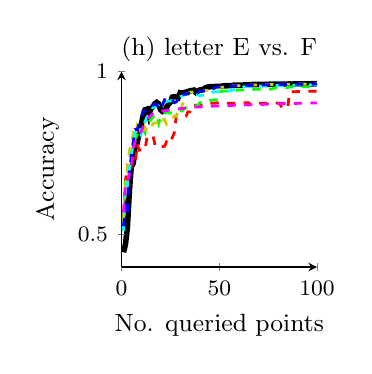
\begin{tikzpicture}

% defining custom colors
\definecolor{mycolor1}{rgb}{0.8,0.8,0}
\definecolor{mycolor2}{rgb}{0,1,1}
\definecolor{mycolor3}{rgb}{1,0,1}


\begin{axis}[
footnotesize,
width= 1.6in,
height= 1.6in,
xmin=0, xmax=100,
ymin=0.4, ymax=1,
title={(h) letter E vs. F},
xlabel = {No. queried points},
ylabel = {Accuracy},
ytick={0.5,1},
xtick = {0,50,100},
axis on top,
axis y line = left,
axis x line = bottom
%legend entries={$optimal$,$rand$,$IVM$,$maxent$,$QBC2$,$QBC100$,$SVM$},
 %egend style={nodes=right}
]
\addplot [
color=black,
solid,
line width=2.0pt
]
coordinates{ (1,0.445429) (2,0.469482) (3,0.521658) (4,0.63165) (5,0.707996) (6,0.718387) (7,0.777472) (8,0.780688) (9,0.810729) (10,0.833312) (11,0.863219) (12,0.882558) (13,0.884406) (14,0.86446) (15,0.886065) (16,0.891593) (17,0.901416) (18,0.905442) (19,0.901287) (20,0.882621) (21,0.877546) (22,0.880332) (23,0.890171) (24,0.899849) (25,0.905665) (26,0.921782) (27,0.922937) (28,0.922789) (29,0.91999) (30,0.935033) (31,0.933756) (32,0.935845) (33,0.936973) (34,0.938507) (35,0.941074) (36,0.941943) (37,0.94313) (38,0.936225) (39,0.941127) (40,0.943364) (41,0.944592) (42,0.945185) (43,0.950627) (44,0.95258) (45,0.953153) (46,0.95391) (47,0.953257) (48,0.954428) (49,0.954462) (50,0.95424) (51,0.955059) (52,0.956203) (53,0.956533) (54,0.956367) (55,0.95676) (56,0.956912) (57,0.957975) (58,0.958211) (59,0.958032) (60,0.958045) (61,0.958152) (62,0.958467) (63,0.959268) (64,0.959397) (65,0.959614) (66,0.960038) (67,0.960345) (68,0.960363) (69,0.960286) (70,0.960334) (71,0.96048) (72,0.960832) (73,0.960525) (74,0.960695) (75,0.960999) (76,0.961225) (77,0.961756) (78,0.961117) (79,0.96113) (80,0.961371) (81,0.961319) (82,0.96127) (83,0.961537) (84,0.961548) (85,0.961752) (86,0.96187) (87,0.961701) (88,0.961935) (89,0.961815) (90,0.961864) (91,0.961942) (92,0.961975) (93,0.962075) (94,0.962224) (95,0.96234) (96,0.962503) (97,0.962608) (98,0.96268) (99,0.962648) (100,0.962732)
};

\addplot [
color=red,
dashed,
line width=1.0pt
]
coordinates{ (1,0.554122) (2,0.663519) (3,0.70985) (4,0.702916) (5,0.708383) (6,0.711151) (7,0.712091) (8,0.77859) (9,0.758533) (10,0.759467) (11,0.758004) (12,0.757855) (13,0.799341) (14,0.800976) (15,0.802867) (16,0.804452) (17,0.778796) (18,0.7797) (19,0.781375) (20,0.769819) (21,0.769998) (22,0.77061) (23,0.784195) (24,0.779142) (25,0.779612) (26,0.798381) (27,0.81197) (28,0.863405) (29,0.864035) (30,0.861872) (31,0.862507) (32,0.862716) (33,0.862804) (34,0.876891) (35,0.87701) (36,0.897389) (37,0.89656) (38,0.89682) (39,0.896844) (40,0.897368) (41,0.897942) (42,0.897979) (43,0.899528) (44,0.902407) (45,0.902501) (46,0.902584) (47,0.903193) (48,0.903176) (49,0.904152) (50,0.904744) (51,0.903067) (52,0.903124) (53,0.903566) (54,0.903054) (55,0.902914) (56,0.903001) (57,0.902978) (58,0.903139) (59,0.903429) (60,0.903606) (61,0.904571) (62,0.904518) (63,0.904638) (64,0.904677) (65,0.904643) (66,0.898919) (67,0.899095) (68,0.89898) (69,0.8991) (70,0.902532) (71,0.902595) (72,0.902587) (73,0.90302) (74,0.903071) (75,0.903148) (76,0.903222) (77,0.903262) (78,0.903246) (79,0.903404) (80,0.903317) (81,0.901617) (82,0.888579) (83,0.888649) (84,0.888723) (85,0.888617) (86,0.938345) (87,0.938256) (88,0.938443) (89,0.938401) (90,0.9385) (91,0.938557) (92,0.938568) (93,0.938624) (94,0.939399) (95,0.939324) (96,0.939345) (97,0.939367) (98,0.939407) (99,0.939448) (100,0.939546)
};

\addplot [
color=green,
dashed,
line width=1.0pt
]
coordinates{ (1,0.536074) (2,0.663881) (3,0.67508) (4,0.728154) (5,0.762147) (6,0.767791) (7,0.793945) (8,0.805811) (9,0.815319) (10,0.820197) (11,0.824374) (12,0.812518) (13,0.845656) (14,0.846473) (15,0.851006) (16,0.862215) (17,0.860649) (18,0.868187) (19,0.841136) (20,0.859657) (21,0.858439) (22,0.871344) (23,0.87544) (24,0.87462) (25,0.872466) (26,0.874423) (27,0.873795) (28,0.877218) (29,0.877748) (30,0.878963) (31,0.879403) (32,0.88602) (33,0.889075) (34,0.889049) (35,0.890444) (36,0.890823) (37,0.892261) (38,0.895257) (39,0.895683) (40,0.904318) (41,0.905439) (42,0.907428) (43,0.907501) (44,0.907371) (45,0.911059) (46,0.911976) (47,0.91242) (48,0.913622) (49,0.913784) (50,0.91398) (51,0.939568) (52,0.94038) (53,0.940459) (54,0.94043) (55,0.942106) (56,0.94239) (57,0.942532) (58,0.942741) (59,0.94299) (60,0.943161) (61,0.943456) (62,0.943357) (63,0.943371) (64,0.944976) (65,0.945056) (66,0.945087) (67,0.945376) (68,0.945402) (69,0.945445) (70,0.945423) (71,0.9454) (72,0.94546) (73,0.945509) (74,0.945508) (75,0.945732) (76,0.946259) (77,0.946499) (78,0.949937) (79,0.949978) (80,0.950021) (81,0.950052) (82,0.950586) (83,0.950709) (84,0.950768) (85,0.950953) (86,0.952899) (87,0.952895) (88,0.952937) (89,0.952861) (90,0.953099) (91,0.953155) (92,0.953238) (93,0.953257) (94,0.95326) (95,0.953551) (96,0.953661) (97,0.953637) (98,0.953637) (99,0.953542) (100,0.950595)
};

\addplot [
color=mycolor1,
dashed,
line width=1.0pt
]
coordinates{ (1,0.539528) (2,0.645249) (3,0.707409) (4,0.757407) (5,0.77917) (6,0.807608) (7,0.79299) (8,0.830992) (9,0.816718) (10,0.817601) (11,0.814776) (12,0.829484) (13,0.81804) (14,0.818646) (15,0.819649) (16,0.839967) (17,0.842257) (18,0.843348) (19,0.841727) (20,0.858482) (21,0.852255) (22,0.853506) (23,0.83842) (24,0.845262) (25,0.855383) (26,0.857954) (27,0.864005) (28,0.862674) (29,0.880769) (30,0.873544) (31,0.897533) (32,0.907412) (33,0.909833) (34,0.932642) (35,0.936487) (36,0.937239) (37,0.929961) (38,0.93497) (39,0.936037) (40,0.936819) (41,0.938728) (42,0.940643) (43,0.94165) (44,0.9426) (45,0.944583) (46,0.946294) (47,0.946194) (48,0.950569) (49,0.951307) (50,0.951225) (51,0.95212) (52,0.952063) (53,0.952906) (54,0.955448) (55,0.955867) (56,0.956079) (57,0.956766) (58,0.956531) (59,0.956832) (60,0.956418) (61,0.956596) (62,0.956638) (63,0.957224) (64,0.958038) (65,0.958335) (66,0.95845) (67,0.958604) (68,0.958604) (69,0.958903) (70,0.959369) (71,0.959336) (72,0.959317) (73,0.960064) (74,0.960224) (75,0.959978) (76,0.960323) (77,0.960653) (78,0.96005) (79,0.960215) (80,0.960241) (81,0.960433) (82,0.960934) (83,0.960968) (84,0.960902) (85,0.960899) (86,0.961077) (87,0.961333) (88,0.96153) (89,0.961393) (90,0.961492) (91,0.961655) (92,0.961683) (93,0.961807) (94,0.961904) (95,0.961918) (96,0.962107) (97,0.96226) (98,0.962305) (99,0.962412) (100,0.962562)
};

\addplot [
color=mycolor2,
dashed,
line width=1.0pt
]
coordinates{ (1,0.510044) (2,0.660234) (3,0.649339) (4,0.699825) (5,0.740787) (6,0.782462) (7,0.81277) (8,0.82197) (9,0.831863) (10,0.809744) (11,0.831762) (12,0.845761) (13,0.860449) (14,0.864866) (15,0.869396) (16,0.888575) (17,0.892327) (18,0.894453) (19,0.89751) (20,0.903777) (21,0.898912) (22,0.902211) (23,0.908218) (24,0.909351) (25,0.909965) (26,0.910648) (27,0.914671) (28,0.920009) (29,0.91996) (30,0.923543) (31,0.924759) (32,0.928488) (33,0.930837) (34,0.92796) (35,0.927802) (36,0.92888) (37,0.928982) (38,0.929471) (39,0.928773) (40,0.92577) (41,0.927554) (42,0.927166) (43,0.929027) (44,0.929374) (45,0.930637) (46,0.934969) (47,0.938019) (48,0.938103) (49,0.937652) (50,0.939449) (51,0.940991) (52,0.942934) (53,0.937752) (54,0.938736) (55,0.940899) (56,0.941381) (57,0.943467) (58,0.946606) (59,0.946395) (60,0.94581) (61,0.948247) (62,0.952493) (63,0.953495) (64,0.953657) (65,0.953756) (66,0.954426) (67,0.954178) (68,0.954643) (69,0.955086) (70,0.955907) (71,0.955758) (72,0.955904) (73,0.955605) (74,0.956121) (75,0.95638) (76,0.956393) (77,0.95674) (78,0.956809) (79,0.956933) (80,0.957134) (81,0.957138) (82,0.957123) (83,0.957156) (84,0.956955) (85,0.957364) (86,0.957336) (87,0.957892) (88,0.957994) (89,0.957966) (90,0.957976) (91,0.958337) (92,0.958633) (93,0.958783) (94,0.958721) (95,0.958501) (96,0.95941) (97,0.959438) (98,0.95943) (99,0.959589) (100,0.959765)
};

\addplot [
color=blue,
dashed,
line width=1.0pt
]
coordinates{ (1,0.525282) (2,0.58521) (3,0.556523) (4,0.687477) (5,0.741077) (6,0.784189) (7,0.822445) (8,0.821136) (9,0.840013) (10,0.850612) (11,0.877717) (12,0.87917) (13,0.877291) (14,0.883193) (15,0.886354) (16,0.897609) (17,0.899832) (18,0.898584) (19,0.887533) (20,0.881879) (21,0.898016) (22,0.913718) (23,0.912188) (24,0.916856) (25,0.920427) (26,0.912973) (27,0.90458) (28,0.906842) (29,0.916751) (30,0.920522) (31,0.918093) (32,0.931826) (33,0.930334) (34,0.932355) (35,0.934181) (36,0.935518) (37,0.938404) (38,0.941436) (39,0.934817) (40,0.938589) (41,0.938739) (42,0.940491) (43,0.941646) (44,0.941622) (45,0.942551) (46,0.943452) (47,0.948593) (48,0.951374) (49,0.952306) (50,0.953098) (51,0.953901) (52,0.953971) (53,0.954328) (54,0.955124) (55,0.955259) (56,0.955879) (57,0.956044) (58,0.95659) (59,0.956594) (60,0.956896) (61,0.95694) (62,0.957458) (63,0.957116) (64,0.957093) (65,0.957133) (66,0.957299) (67,0.957928) (68,0.958066) (69,0.958467) (70,0.958557) (71,0.958553) (72,0.958552) (73,0.958497) (74,0.959409) (75,0.959427) (76,0.959461) (77,0.959492) (78,0.959894) (79,0.960012) (80,0.960215) (81,0.960402) (82,0.960503) (83,0.96061) (84,0.96062) (85,0.960689) (86,0.960676) (87,0.960664) (88,0.960832) (89,0.960843) (90,0.960901) (91,0.960871) (92,0.960914) (93,0.961032) (94,0.961084) (95,0.961182) (96,0.961156) (97,0.961121) (98,0.961442) (99,0.961648) (100,0.961702)
};

\addplot [
color=mycolor3,
dashed,
line width=1.0pt
]
coordinates{ (1,0.568292) (2,0.65376) (3,0.654767) (4,0.685808) (5,0.694862) (6,0.766994) (7,0.785344) (8,0.799123) (9,0.808101) (10,0.815711) (11,0.82999) (12,0.836492) (13,0.84344) (14,0.860353) (15,0.865131) (16,0.87075) (17,0.874529) (18,0.875742) (19,0.876848) (20,0.877883) (21,0.878999) (22,0.879863) (23,0.880332) (24,0.881482) (25,0.882128) (26,0.882665) (27,0.883598) (28,0.884975) (29,0.885479) (30,0.886056) (31,0.886699) (32,0.887332) (33,0.887697) (34,0.888233) (35,0.889398) (36,0.89038) (37,0.890687) (38,0.891139) (39,0.891196) (40,0.891054) (41,0.89176) (42,0.891899) (43,0.89242) (44,0.89286) (45,0.893253) (46,0.893514) (47,0.893984) (48,0.89425) (49,0.894) (50,0.89426) (51,0.894436) (52,0.895127) (53,0.895288) (54,0.895738) (55,0.895455) (56,0.895821) (57,0.896242) (58,0.897187) (59,0.897474) (60,0.897466) (61,0.897725) (62,0.897831) (63,0.89778) (64,0.897899) (65,0.897721) (66,0.897903) (67,0.897993) (68,0.898144) (69,0.898353) (70,0.898839) (71,0.898937) (72,0.899206) (73,0.899415) (74,0.899748) (75,0.900205) (76,0.900265) (77,0.900694) (78,0.900744) (79,0.901055) (80,0.901249) (81,0.90155) (82,0.901693) (83,0.90189) (84,0.901934) (85,0.902338) (86,0.902417) (87,0.902514) (88,0.902494) (89,0.902302) (90,0.902438) (91,0.902549) (92,0.902496) (93,0.902764) (94,0.902826) (95,0.902949) (96,0.903626) (97,0.903555) (98,0.903618) (99,0.903758) (100,0.903843)
};

\end{axis}
\end{tikzpicture}
&
% This file was created by matlab2tikz v0.0.7.
% Copyright (c) 2008--2010, Nico Schlömer <nico.schloemer@gmail.com>
% All rights reserved.
% 
% The latest updates can be retrieved from
%   http://www.mathworks.com/matlabcentral/fileexchange/22022-matlab2tikz
% where you can also make suggestions and rate matlab2tikz.
% 
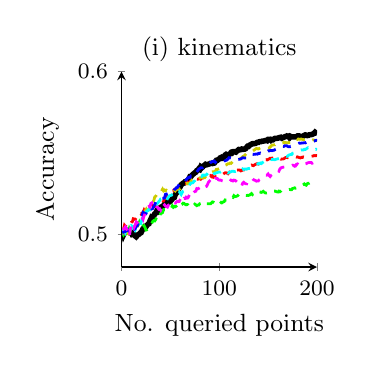
\begin{tikzpicture}

% defining custom colors
\definecolor{mycolor1}{rgb}{0.8,0.8,0}
\definecolor{mycolor2}{rgb}{0,1,1}
\definecolor{mycolor3}{rgb}{1,0,1}


\begin{axis}[
footnotesize,
width= 1.6in,
height= 1.6in,
xmin=0, xmax=200,
ymin=0.48, ymax=0.6,
ytick={0.5,0.6},
xtick = {0,100,200},
title = {(i) kinematics},
xlabel = {No. queried points},
ylabel = {Accuracy},
axis on top,
axis y line = left,
axis x line = bottom
%legend entries={$optimal$,$rand$,$IVM$,$maxent$,$QBC2$,$QBC100$,$SVM$},
 %egend style={nodes=right}
]
\addplot [
color=black,
solid,
line width=2.0pt
]
coordinates{ (1,0.501837) (2,0.49981) (3,0.501099) (4,0.501695) (5,0.502288) (6,0.502279) (7,0.50162) (8,0.501309) (9,0.501497) (10,0.501282) (11,0.499943) (12,0.500053) (13,0.499904) (14,0.499106) (15,0.49862) (16,0.499285) (17,0.499876) (18,0.500184) (19,0.500877) (20,0.50112) (21,0.502335) (22,0.503583) (23,0.504014) (24,0.504904) (25,0.50478) (26,0.505628) (27,0.506218) (28,0.506557) (29,0.508157) (30,0.509362) (31,0.510867) (32,0.510714) (33,0.511313) (34,0.512717) (35,0.5131) (36,0.514364) (37,0.514042) (38,0.514937) (39,0.515419) (40,0.516699) (41,0.516947) (42,0.516889) (43,0.517819) (44,0.518576) (45,0.519136) (46,0.520306) (47,0.520601) (48,0.519903) (49,0.51998) (50,0.520423) (51,0.521074) (52,0.521845) (53,0.522556) (54,0.522759) (55,0.524486) (56,0.525295) (57,0.526057) (58,0.52744) (59,0.52844) (60,0.529193) (61,0.530489) (62,0.530983) (63,0.531461) (64,0.531587) (65,0.532406) (66,0.532595) (67,0.532828) (68,0.533341) (69,0.534307) (70,0.535483) (71,0.5355) (72,0.536303) (73,0.536939) (74,0.537329) (75,0.537922) (76,0.538208) (77,0.539155) (78,0.539462) (79,0.54023) (80,0.53993) (81,0.541396) (82,0.540888) (83,0.541445) (84,0.542161) (85,0.542498) (86,0.543056) (87,0.542801) (88,0.542966) (89,0.543114) (90,0.543317) (91,0.543686) (92,0.54371) (93,0.54355) (94,0.543719) (95,0.543873) (96,0.544658) (97,0.545503) (98,0.545504) (99,0.546019) (100,0.546322) (101,0.547039) (102,0.547326) (103,0.546754) (104,0.54685) (105,0.547529) (106,0.548764) (107,0.549166) (108,0.548816) (109,0.548706) (110,0.548899) (111,0.549579) (112,0.550249) (113,0.550028) (114,0.5508) (115,0.550887) (116,0.550761) (117,0.550581) (118,0.551123) (119,0.55159) (120,0.552128) (121,0.551969) (122,0.552111) (123,0.552441) (124,0.552248) (125,0.552364) (126,0.552393) (127,0.552679) (128,0.553504) (129,0.554167) (130,0.554099) (131,0.554826) (132,0.555058) (133,0.555489) (134,0.555696) (135,0.555706) (136,0.555812) (137,0.555895) (138,0.556215) (139,0.556538) (140,0.556504) (141,0.556914) (142,0.556952) (143,0.557052) (144,0.557298) (145,0.55734) (146,0.557419) (147,0.557661) (148,0.557795) (149,0.55757) (150,0.558318) (151,0.558289) (152,0.558397) (153,0.557814) (154,0.558253) (155,0.558177) (156,0.558635) (157,0.559013) (158,0.558976) (159,0.559039) (160,0.559125) (161,0.559365) (162,0.55956) (163,0.55969) (164,0.559132) (165,0.559357) (166,0.559653) (167,0.559977) (168,0.560194) (169,0.560455) (170,0.560129) (171,0.560347) (172,0.559477) (173,0.560197) (174,0.559927) (175,0.559873) (176,0.559935) (177,0.559862) (178,0.559923) (179,0.560081) (180,0.560487) (181,0.560543) (182,0.560453) (183,0.56002) (184,0.560123) (185,0.560257) (186,0.560415) (187,0.560862) (188,0.561119) (189,0.560944) (190,0.560738) (191,0.560785) (192,0.561178) (193,0.561229) (194,0.561283) (195,0.56141) (196,0.561759) (197,0.562057) (198,0.562743) (199,0.562293) (200,0.562154)
};

\addplot [
color=red,
dashed,
line width=1.0pt
]
coordinates{ (1,0.503748) (2,0.503349) (3,0.505721) (4,0.504997) (5,0.505936) (6,0.506005) (7,0.504912) (8,0.505023) (9,0.506014) (10,0.507419) (11,0.507727) (12,0.509651) (13,0.509437) (14,0.509243) (15,0.510176) (16,0.510556) (17,0.511285) (18,0.512348) (19,0.513426) (20,0.512513) (21,0.513089) (22,0.513589) (23,0.514997) (24,0.513934) (25,0.515051) (26,0.515665) (27,0.516442) (28,0.516767) (29,0.517308) (30,0.517966) (31,0.518135) (32,0.517758) (33,0.517203) (34,0.517242) (35,0.517504) (36,0.519956) (37,0.520469) (38,0.520318) (39,0.52017) (40,0.521067) (41,0.521138) (42,0.520653) (43,0.520571) (44,0.521751) (45,0.522121) (46,0.523584) (47,0.524969) (48,0.524823) (49,0.525533) (50,0.525169) (51,0.526208) (52,0.526644) (53,0.526803) (54,0.52759) (55,0.527914) (56,0.527747) (57,0.527587) (58,0.528606) (59,0.528675) (60,0.52873) (61,0.529586) (62,0.52972) (63,0.53059) (64,0.530687) (65,0.531335) (66,0.531218) (67,0.532356) (68,0.531861) (69,0.531776) (70,0.532331) (71,0.531797) (72,0.531854) (73,0.531646) (74,0.531153) (75,0.532297) (76,0.533189) (77,0.534009) (78,0.533901) (79,0.534055) (80,0.534454) (81,0.533981) (82,0.534745) (83,0.534606) (84,0.535057) (85,0.535171) (86,0.535888) (87,0.535728) (88,0.536508) (89,0.535578) (90,0.536155) (91,0.53626) (92,0.535523) (93,0.535968) (94,0.535064) (95,0.535344) (96,0.535506) (97,0.53521) (98,0.534868) (99,0.535246) (100,0.535715) (101,0.536032) (102,0.536397) (103,0.536776) (104,0.537054) (105,0.537491) (106,0.537895) (107,0.537867) (108,0.537611) (109,0.537282) (110,0.537998) (111,0.538571) (112,0.538862) (113,0.539219) (114,0.539915) (115,0.539615) (116,0.539909) (117,0.539911) (118,0.539453) (119,0.53955) (120,0.539512) (121,0.539553) (122,0.539029) (123,0.53925) (124,0.539681) (125,0.53956) (126,0.539903) (127,0.540355) (128,0.540584) (129,0.541138) (130,0.54144) (131,0.541485) (132,0.542302) (133,0.542643) (134,0.5424) (135,0.542259) (136,0.542697) (137,0.543) (138,0.543349) (139,0.543476) (140,0.543245) (141,0.54401) (142,0.544313) (143,0.544539) (144,0.544825) (145,0.545204) (146,0.545542) (147,0.545819) (148,0.545933) (149,0.545728) (150,0.546064) (151,0.54641) (152,0.546776) (153,0.546535) (154,0.546912) (155,0.546893) (156,0.547341) (157,0.547223) (158,0.547136) (159,0.547609) (160,0.547377) (161,0.547027) (162,0.5466) (163,0.546202) (164,0.546305) (165,0.546291) (166,0.546504) (167,0.546851) (168,0.547309) (169,0.547341) (170,0.547129) (171,0.547247) (172,0.54715) (173,0.547003) (174,0.5475) (175,0.547716) (176,0.547692) (177,0.547877) (178,0.547674) (179,0.547488) (180,0.547632) (181,0.54736) (182,0.547159) (183,0.546995) (184,0.547343) (185,0.547243) (186,0.547609) (187,0.547401) (188,0.547069) (189,0.547146) (190,0.547245) (191,0.547282) (192,0.547445) (193,0.547823) (194,0.547978) (195,0.548083) (196,0.548153) (197,0.54847) (198,0.548319) (199,0.548469) (200,0.548354)
};

\addplot [
color=green,
dashed,
line width=1.0pt
]
coordinates{ (1,0.500858) (2,0.499771) (3,0.500791) (4,0.502165) (5,0.501305) (6,0.503165) (7,0.501139) (8,0.503655) (9,0.502334) (10,0.503569) (11,0.504324) (12,0.505387) (13,0.505173) (14,0.505745) (15,0.504466) (16,0.506778) (17,0.505993) (18,0.507349) (19,0.505166) (20,0.506534) (21,0.504647) (22,0.505352) (23,0.505428) (24,0.504378) (25,0.502706) (26,0.502871) (27,0.503383) (28,0.505849) (29,0.5058) (30,0.506062) (31,0.506957) (32,0.508071) (33,0.508542) (34,0.508309) (35,0.509188) (36,0.510859) (37,0.511362) (38,0.512451) (39,0.510987) (40,0.512856) (41,0.513033) (42,0.51347) (43,0.51527) (44,0.515333) (45,0.515284) (46,0.515045) (47,0.514963) (48,0.515771) (49,0.515507) (50,0.516266) (51,0.516234) (52,0.517587) (53,0.516669) (54,0.51717) (55,0.517008) (56,0.517389) (57,0.517888) (58,0.51886) (59,0.517919) (60,0.519046) (61,0.518173) (62,0.518501) (63,0.519225) (64,0.519046) (65,0.518532) (66,0.518216) (67,0.518465) (68,0.518238) (69,0.517626) (70,0.51896) (71,0.518839) (72,0.519136) (73,0.518235) (74,0.517987) (75,0.518639) (76,0.518204) (77,0.517705) (78,0.518059) (79,0.518073) (80,0.518892) (81,0.519097) (82,0.518142) (83,0.518658) (84,0.518609) (85,0.518186) (86,0.518159) (87,0.518906) (88,0.518923) (89,0.518812) (90,0.518797) (91,0.518799) (92,0.519415) (93,0.520006) (94,0.519872) (95,0.519439) (96,0.519315) (97,0.51864) (98,0.519056) (99,0.518017) (100,0.51833) (101,0.51897) (102,0.519759) (103,0.519515) (104,0.519969) (105,0.520166) (106,0.521226) (107,0.52118) (108,0.521222) (109,0.522404) (110,0.5223) (111,0.521955) (112,0.521953) (113,0.522873) (114,0.522698) (115,0.523813) (116,0.523241) (117,0.523316) (118,0.52353) (119,0.523851) (120,0.524469) (121,0.524801) (122,0.524561) (123,0.524043) (124,0.524452) (125,0.524103) (126,0.524392) (127,0.524024) (128,0.523956) (129,0.524015) (130,0.523995) (131,0.524161) (132,0.524611) (133,0.525161) (134,0.524576) (135,0.52552) (136,0.525433) (137,0.525534) (138,0.525739) (139,0.525682) (140,0.525265) (141,0.526135) (142,0.526038) (143,0.525819) (144,0.526087) (145,0.526517) (146,0.525987) (147,0.525529) (148,0.525446) (149,0.525533) (150,0.525926) (151,0.525475) (152,0.525878) (153,0.525958) (154,0.526535) (155,0.52645) (156,0.526605) (157,0.526638) (158,0.526404) (159,0.526153) (160,0.526045) (161,0.526596) (162,0.526219) (163,0.526668) (164,0.527282) (165,0.526862) (166,0.52699) (167,0.527236) (168,0.527171) (169,0.527267) (170,0.527263) (171,0.527463) (172,0.527657) (173,0.52744) (174,0.527408) (175,0.528262) (176,0.528329) (177,0.528633) (178,0.528408) (179,0.528533) (180,0.52915) (181,0.529585) (182,0.529097) (183,0.529396) (184,0.530057) (185,0.530383) (186,0.530651) (187,0.531042) (188,0.530497) (189,0.530231) (190,0.531129) (191,0.53148) (192,0.531451) (193,0.531855) (194,0.532164) (195,0.531997) (196,0.531888) (197,0.53202) (198,0.532191) (199,0.532478) (200,0.532415)
};

\addplot [
color=mycolor1,
dashed,
line width=1.0pt
]
coordinates{ (1,0.501256) (2,0.501375) (3,0.501298) (4,0.502102) (5,0.501147) (6,0.500906) (7,0.500412) (8,0.501468) (9,0.502017) (10,0.502218) (11,0.503351) (12,0.503787) (13,0.50382) (14,0.504821) (15,0.505324) (16,0.50555) (17,0.505795) (18,0.508579) (19,0.509195) (20,0.50993) (21,0.51115) (22,0.511578) (23,0.512522) (24,0.513987) (25,0.515279) (26,0.516255) (27,0.516355) (28,0.517178) (29,0.517484) (30,0.518021) (31,0.518669) (32,0.519849) (33,0.520773) (34,0.523068) (35,0.523479) (36,0.524451) (37,0.525853) (38,0.525388) (39,0.525232) (40,0.526121) (41,0.526669) (42,0.527822) (43,0.526784) (44,0.527285) (45,0.526826) (46,0.527199) (47,0.526883) (48,0.527481) (49,0.527992) (50,0.527307) (51,0.527471) (52,0.527805) (53,0.527814) (54,0.527343) (55,0.526769) (56,0.527753) (57,0.527818) (58,0.527709) (59,0.528066) (60,0.527947) (61,0.52879) (62,0.530034) (63,0.530764) (64,0.531166) (65,0.531139) (66,0.531116) (67,0.531469) (68,0.531068) (69,0.531389) (70,0.531546) (71,0.532562) (72,0.533397) (73,0.533108) (74,0.532959) (75,0.533244) (76,0.533239) (77,0.533645) (78,0.534507) (79,0.534095) (80,0.534639) (81,0.534698) (82,0.534948) (83,0.535136) (84,0.534829) (85,0.534787) (86,0.535532) (87,0.536374) (88,0.537328) (89,0.537365) (90,0.537193) (91,0.537887) (92,0.538225) (93,0.538514) (94,0.538531) (95,0.538574) (96,0.538939) (97,0.539963) (98,0.539861) (99,0.540212) (100,0.540424) (101,0.540947) (102,0.541752) (103,0.5423) (104,0.542133) (105,0.542719) (106,0.542524) (107,0.542681) (108,0.543061) (109,0.54342) (110,0.543374) (111,0.54382) (112,0.543651) (113,0.544175) (114,0.544782) (115,0.544829) (116,0.545376) (117,0.545564) (118,0.545607) (119,0.54544) (120,0.545651) (121,0.546333) (122,0.546616) (123,0.547179) (124,0.547857) (125,0.548193) (126,0.548411) (127,0.549207) (128,0.549909) (129,0.550375) (130,0.550805) (131,0.550604) (132,0.550911) (133,0.550748) (134,0.551139) (135,0.551541) (136,0.551939) (137,0.552397) (138,0.552846) (139,0.552576) (140,0.552479) (141,0.552843) (142,0.553135) (143,0.553189) (144,0.553091) (145,0.552834) (146,0.552813) (147,0.552396) (148,0.552587) (149,0.55289) (150,0.55291) (151,0.553079) (152,0.553661) (153,0.554317) (154,0.554853) (155,0.55495) (156,0.555029) (157,0.55508) (158,0.555808) (159,0.555709) (160,0.555782) (161,0.555567) (162,0.555834) (163,0.556198) (164,0.556104) (165,0.556233) (166,0.556598) (167,0.55626) (168,0.556497) (169,0.556246) (170,0.556261) (171,0.556247) (172,0.556709) (173,0.556984) (174,0.556466) (175,0.556685) (176,0.556842) (177,0.557412) (178,0.558099) (179,0.558548) (180,0.558342) (181,0.558628) (182,0.558464) (183,0.558512) (184,0.558596) (185,0.558314) (186,0.558271) (187,0.558318) (188,0.558531) (189,0.558535) (190,0.558013) (191,0.55789) (192,0.557829) (193,0.55814) (194,0.557946) (195,0.557763) (196,0.558087) (197,0.557922) (198,0.557682) (199,0.5577) (200,0.557876)
};

\addplot [
color=mycolor2,
dashed,
line width=1.0pt
]
coordinates{ (1,0.501412) (2,0.502767) (3,0.503413) (4,0.50156) (5,0.503243) (6,0.504458) (7,0.504597) (8,0.504754) (9,0.504606) (10,0.505461) (11,0.505102) (12,0.504084) (13,0.504651) (14,0.502898) (15,0.504196) (16,0.504018) (17,0.504792) (18,0.504386) (19,0.505547) (20,0.50732) (21,0.509499) (22,0.511919) (23,0.51233) (24,0.511348) (25,0.513381) (26,0.514444) (27,0.51459) (28,0.515517) (29,0.515177) (30,0.516018) (31,0.516847) (32,0.517217) (33,0.518069) (34,0.51904) (35,0.517746) (36,0.518929) (37,0.519245) (38,0.52014) (39,0.520814) (40,0.521749) (41,0.52166) (42,0.521594) (43,0.521131) (44,0.52196) (45,0.520854) (46,0.520883) (47,0.522015) (48,0.522997) (49,0.523675) (50,0.523945) (51,0.524077) (52,0.524802) (53,0.524872) (54,0.524143) (55,0.525175) (56,0.525382) (57,0.525713) (58,0.525924) (59,0.526254) (60,0.525419) (61,0.524541) (62,0.525723) (63,0.526573) (64,0.526893) (65,0.527801) (66,0.528068) (67,0.528567) (68,0.529404) (69,0.529736) (70,0.530808) (71,0.531604) (72,0.531652) (73,0.531738) (74,0.532516) (75,0.532991) (76,0.533995) (77,0.535281) (78,0.535391) (79,0.535441) (80,0.536087) (81,0.535902) (82,0.535643) (83,0.536437) (84,0.536528) (85,0.536293) (86,0.536503) (87,0.536758) (88,0.537431) (89,0.53817) (90,0.538194) (91,0.53725) (92,0.536792) (93,0.537773) (94,0.538094) (95,0.537472) (96,0.537505) (97,0.537905) (98,0.537987) (99,0.53824) (100,0.538378) (101,0.538238) (102,0.538551) (103,0.538626) (104,0.538529) (105,0.539172) (106,0.539133) (107,0.53903) (108,0.538446) (109,0.537805) (110,0.538213) (111,0.538333) (112,0.538471) (113,0.53878) (114,0.538789) (115,0.53872) (116,0.538601) (117,0.538797) (118,0.539074) (119,0.539595) (120,0.538889) (121,0.538917) (122,0.539028) (123,0.539545) (124,0.540233) (125,0.539858) (126,0.540201) (127,0.54017) (128,0.540045) (129,0.540367) (130,0.540523) (131,0.540556) (132,0.540708) (133,0.540612) (134,0.541312) (135,0.541561) (136,0.542211) (137,0.542431) (138,0.542483) (139,0.543049) (140,0.543586) (141,0.543338) (142,0.543838) (143,0.543541) (144,0.544115) (145,0.544439) (146,0.544906) (147,0.545032) (148,0.545586) (149,0.54599) (150,0.546338) (151,0.546004) (152,0.546208) (153,0.546021) (154,0.545933) (155,0.546051) (156,0.545926) (157,0.545927) (158,0.546179) (159,0.546297) (160,0.546511) (161,0.546472) (162,0.546757) (163,0.547056) (164,0.54777) (165,0.547726) (166,0.547761) (167,0.547848) (168,0.548057) (169,0.547922) (170,0.548169) (171,0.548628) (172,0.548961) (173,0.549036) (174,0.549046) (175,0.549851) (176,0.550006) (177,0.550347) (178,0.550434) (179,0.550827) (180,0.550968) (181,0.551277) (182,0.551833) (183,0.551728) (184,0.551936) (185,0.551798) (186,0.551873) (187,0.55231) (188,0.552179) (189,0.552545) (190,0.553009) (191,0.553299) (192,0.553166) (193,0.552832) (194,0.552808) (195,0.55288) (196,0.552792) (197,0.552102) (198,0.551948) (199,0.552328) (200,0.551968)
};

\addplot [
color=blue,
dashed,
line width=1.0pt
]
coordinates{ (1,0.502102) (2,0.501409) (3,0.501685) (4,0.501823) (5,0.502479) (6,0.503092) (7,0.502361) (8,0.503032) (9,0.503397) (10,0.502596) (11,0.504006) (12,0.503783) (13,0.503123) (14,0.50356) (15,0.504998) (16,0.505116) (17,0.506582) (18,0.509039) (19,0.509999) (20,0.511196) (21,0.511741) (22,0.513532) (23,0.513227) (24,0.512993) (25,0.512779) (26,0.513997) (27,0.51473) (28,0.515862) (29,0.516263) (30,0.516631) (31,0.515711) (32,0.515968) (33,0.51729) (34,0.518281) (35,0.51992) (36,0.520301) (37,0.520972) (38,0.521417) (39,0.521894) (40,0.521809) (41,0.522182) (42,0.522167) (43,0.522182) (44,0.522447) (45,0.524752) (46,0.524753) (47,0.52508) (48,0.525355) (49,0.525595) (50,0.5264) (51,0.526158) (52,0.526091) (53,0.526198) (54,0.527457) (55,0.527874) (56,0.528694) (57,0.528662) (58,0.529876) (59,0.530579) (60,0.531533) (61,0.531128) (62,0.531593) (63,0.531545) (64,0.532173) (65,0.532284) (66,0.533555) (67,0.534074) (68,0.534847) (69,0.535159) (70,0.534996) (71,0.535828) (72,0.535462) (73,0.536071) (74,0.536215) (75,0.537325) (76,0.537401) (77,0.538366) (78,0.539151) (79,0.540139) (80,0.540501) (81,0.540922) (82,0.540963) (83,0.540947) (84,0.541724) (85,0.542111) (86,0.542539) (87,0.542677) (88,0.5428) (89,0.542978) (90,0.543443) (91,0.544176) (92,0.544386) (93,0.54486) (94,0.544788) (95,0.54506) (96,0.544308) (97,0.54504) (98,0.545118) (99,0.545159) (100,0.545124) (101,0.545206) (102,0.5453) (103,0.545731) (104,0.545934) (105,0.54587) (106,0.545266) (107,0.545552) (108,0.545758) (109,0.546353) (110,0.547153) (111,0.547107) (112,0.546973) (113,0.546858) (114,0.546494) (115,0.546693) (116,0.547109) (117,0.546596) (118,0.546316) (119,0.54606) (120,0.546123) (121,0.546213) (122,0.546339) (123,0.546749) (124,0.547109) (125,0.547028) (126,0.546881) (127,0.546906) (128,0.546895) (129,0.547463) (130,0.547451) (131,0.548062) (132,0.548191) (133,0.548197) (134,0.54918) (135,0.54916) (136,0.549284) (137,0.54931) (138,0.549392) (139,0.549279) (140,0.549785) (141,0.549742) (142,0.549996) (143,0.549666) (144,0.549575) (145,0.549591) (146,0.549721) (147,0.550164) (148,0.550504) (149,0.550758) (150,0.551349) (151,0.551255) (152,0.551563) (153,0.551594) (154,0.551446) (155,0.551606) (156,0.551717) (157,0.55206) (158,0.552311) (159,0.552493) (160,0.552632) (161,0.55256) (162,0.553159) (163,0.553742) (164,0.553754) (165,0.554119) (166,0.55403) (167,0.55443) (168,0.554509) (169,0.554443) (170,0.554048) (171,0.553824) (172,0.553802) (173,0.554097) (174,0.554108) (175,0.554278) (176,0.554671) (177,0.554807) (178,0.555234) (179,0.555398) (180,0.555638) (181,0.555894) (182,0.556077) (183,0.555985) (184,0.556082) (185,0.556099) (186,0.556216) (187,0.556315) (188,0.556225) (189,0.556594) (190,0.556897) (191,0.556772) (192,0.556861) (193,0.556377) (194,0.556521) (195,0.556885) (196,0.55705) (197,0.55726) (198,0.55761) (199,0.557819) (200,0.55759)
};

\addplot [
color=mycolor3,
dashed,
line width=1.0pt
]
coordinates{ (1,0.502864) (2,0.503209) (3,0.503703) (4,0.504644) (5,0.503654) (6,0.502324) (7,0.50147) (8,0.498684) (9,0.503113) (10,0.505718) (11,0.507133) (12,0.506388) (13,0.504546) (14,0.505843) (15,0.507747) (16,0.507363) (17,0.508814) (18,0.50998) (19,0.511147) (20,0.511348) (21,0.510263) (22,0.509278) (23,0.511394) (24,0.51264) (25,0.515396) (26,0.515439) (27,0.516854) (28,0.517237) (29,0.51683) (30,0.519034) (31,0.519339) (32,0.517357) (33,0.516091) (34,0.515839) (35,0.517381) (36,0.516892) (37,0.516674) (38,0.5156) (39,0.515873) (40,0.514937) (41,0.516224) (42,0.514699) (43,0.517538) (44,0.518209) (45,0.517431) (46,0.517169) (47,0.516837) (48,0.517994) (49,0.518298) (50,0.517005) (51,0.518269) (52,0.518998) (53,0.51933) (54,0.519326) (55,0.519274) (56,0.519963) (57,0.52032) (58,0.520139) (59,0.520235) (60,0.521449) (61,0.522477) (62,0.520433) (63,0.521335) (64,0.522173) (65,0.522062) (66,0.522856) (67,0.522292) (68,0.52246) (69,0.523727) (70,0.52485) (71,0.526289) (72,0.526488) (73,0.525247) (74,0.525908) (75,0.526331) (76,0.526535) (77,0.528183) (78,0.528018) (79,0.528306) (80,0.528702) (81,0.528782) (82,0.528535) (83,0.529827) (84,0.530206) (85,0.529924) (86,0.529208) (87,0.529558) (88,0.530692) (89,0.532117) (90,0.532775) (91,0.532112) (92,0.531223) (93,0.532077) (94,0.532643) (95,0.533359) (96,0.534374) (97,0.534401) (98,0.534344) (99,0.533677) (100,0.533332) (101,0.533429) (102,0.533233) (103,0.532941) (104,0.532752) (105,0.533099) (106,0.533359) (107,0.533246) (108,0.533484) (109,0.53332) (110,0.533354) (111,0.532693) (112,0.533399) (113,0.533172) (114,0.532866) (115,0.533352) (116,0.533241) (117,0.532893) (118,0.532286) (119,0.530431) (120,0.529585) (121,0.52946) (122,0.529824) (123,0.529986) (124,0.531563) (125,0.532032) (126,0.531447) (127,0.531089) (128,0.53107) (129,0.532471) (130,0.533711) (131,0.533629) (132,0.533606) (133,0.533927) (134,0.53431) (135,0.533623) (136,0.533325) (137,0.533143) (138,0.532731) (139,0.532816) (140,0.532869) (141,0.533586) (142,0.533949) (143,0.533988) (144,0.534546) (145,0.535498) (146,0.536227) (147,0.536407) (148,0.536326) (149,0.536485) (150,0.537128) (151,0.536108) (152,0.535541) (153,0.536278) (154,0.536727) (155,0.537408) (156,0.537945) (157,0.538487) (158,0.53927) (159,0.539388) (160,0.539191) (161,0.538847) (162,0.540155) (163,0.540873) (164,0.541075) (165,0.541261) (166,0.541352) (167,0.541403) (168,0.541674) (169,0.541672) (170,0.541882) (171,0.542258) (172,0.54242) (173,0.54207) (174,0.542311) (175,0.542564) (176,0.542454) (177,0.541845) (178,0.541965) (179,0.543063) (180,0.543335) (181,0.542962) (182,0.542992) (183,0.543317) (184,0.543639) (185,0.543069) (186,0.543021) (187,0.542713) (188,0.543314) (189,0.543462) (190,0.543852) (191,0.544081) (192,0.544151) (193,0.544172) (194,0.544182) (195,0.543712) (196,0.543992) (197,0.54426) (198,0.544515) (199,0.544858) (200,0.545029)
};

\end{axis}
\end{tikzpicture}
\\
% This file was created by matlab2tikz v0.0.7.
% Copyright (c) 2008--2010, Nico Schlömer <nico.schloemer@gmail.com>
% All rights reserved.
% 
% The latest updates can be retrieved from
%   http://www.mathworks.com/matlabcentral/fileexchange/22022-matlab2tikz
% where you can also make suggestions and rate matlab2tikz.
% 
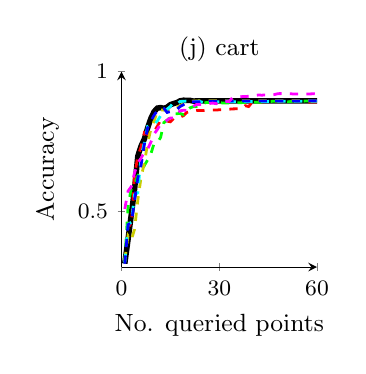
\begin{tikzpicture}

% defining custom colors
\definecolor{mycolor1}{rgb}{0.8,0.8,0}
\definecolor{mycolor2}{rgb}{0,1,1}
\definecolor{mycolor3}{rgb}{1,0,1}


\begin{axis}[
footnotesize,
width= 1.6in,
height= 1.6in,
xmin=0, xmax=60,
ymin=0.3, ymax=1,
ytick={0.5,1},
xtick = {0,30,60},
title = {(j) cart},
xlabel = {No. queried points},
ylabel = {Accuracy},
axis on top,
axis y line = left,
axis x line = bottom
%legend entries={$optimal$,$rand$,$IVM$,$maxent$,$QBC2$,$QBC100$,$SVM$},
 %egend style={nodes=right}
]
\addplot [
color=black,
solid,
line width=2.0pt
]
coordinates{ (1,0.312526) (2,0.399241) (3,0.488004) (4,0.579085) (5,0.697324) (6,0.733291) (7,0.758203) (8,0.797845) (9,0.832066) (10,0.856567) (11,0.869124) (12,0.870926) (13,0.868264) (14,0.872361) (15,0.881437) (16,0.885509) (17,0.889029) (18,0.895204) (19,0.897279) (20,0.897242) (21,0.89693) (22,0.894416) (23,0.894739) (24,0.894949) (25,0.894928) (26,0.894783) (27,0.894781) (28,0.894945) (29,0.895026) (30,0.895063) (31,0.895116) (32,0.895236) (33,0.895336) (34,0.895315) (35,0.89531) (36,0.895292) (37,0.895285) (38,0.895268) (39,0.895304) (40,0.895326) (41,0.895339) (42,0.895337) (43,0.895339) (44,0.895361) (45,0.895356) (46,0.895363) (47,0.895384) (48,0.895385) (49,0.895366) (50,0.895393) (51,0.895392) (52,0.895398) (53,0.895392) (54,0.895397) (55,0.895416) (56,0.89541) (57,0.895433) (58,0.895443) (59,0.895426) (60,0.895436)
};

\addplot [
color=red,
dashed,
line width=1.0pt
]
coordinates{ (1,0.318594) (2,0.454087) (3,0.448753) (4,0.630239) (5,0.69573) (6,0.730708) (7,0.780788) (8,0.774727) (9,0.785811) (10,0.786118) (11,0.804199) (12,0.826249) (13,0.824891) (14,0.822457) (15,0.820244) (16,0.832063) (17,0.831762) (18,0.836923) (19,0.842141) (20,0.853597) (21,0.857272) (22,0.857588) (23,0.860348) (24,0.860955) (25,0.860765) (26,0.861416) (27,0.862279) (28,0.862462) (29,0.862629) (30,0.862984) (31,0.86397) (32,0.864076) (33,0.86512) (34,0.866372) (35,0.866519) (36,0.86687) (37,0.865979) (38,0.877618) (39,0.874625) (40,0.88881) (41,0.889859) (42,0.890983) (43,0.891555) (44,0.892781) (45,0.895308) (46,0.890701) (47,0.892242) (48,0.892879) (49,0.89313) (50,0.893901) (51,0.893937) (52,0.894954) (53,0.895014) (54,0.894861) (55,0.892759) (56,0.890177) (57,0.890174) (58,0.890832) (59,0.890841) (60,0.891391)
};

\addplot [
color=green,
dashed,
line width=1.0pt
]
coordinates{ (1,0.314429) (2,0.519428) (3,0.582174) (4,0.596367) (5,0.627429) (6,0.639234) (7,0.663735) (8,0.68313) (9,0.704864) (10,0.743134) (11,0.745635) (12,0.764256) (13,0.817531) (14,0.825799) (15,0.837663) (16,0.84922) (17,0.84917) (18,0.849989) (19,0.845572) (20,0.859836) (21,0.869851) (22,0.874449) (23,0.875224) (24,0.884028) (25,0.885637) (26,0.889163) (27,0.889393) (28,0.890345) (29,0.891669) (30,0.889276) (31,0.887453) (32,0.887372) (33,0.887786) (34,0.887787) (35,0.887941) (36,0.887997) (37,0.888957) (38,0.889098) (39,0.88948) (40,0.88985) (41,0.890063) (42,0.890083) (43,0.890755) (44,0.891686) (45,0.892638) (46,0.893253) (47,0.89365) (48,0.893681) (49,0.893749) (50,0.894371) (51,0.891564) (52,0.892911) (53,0.893893) (54,0.893875) (55,0.894071) (56,0.89418) (57,0.894391) (58,0.894359) (59,0.894355) (60,0.894368)
};

\addplot [
color=mycolor1,
dashed,
line width=1.0pt
]
coordinates{ (1,0.324707) (2,0.41235) (3,0.39674) (4,0.435539) (5,0.539376) (6,0.622108) (7,0.671762) (8,0.742547) (9,0.79335) (10,0.822596) (11,0.858366) (12,0.862154) (13,0.86272) (14,0.862225) (15,0.861586) (16,0.872173) (17,0.873321) (18,0.877967) (19,0.884751) (20,0.890098) (21,0.892173) (22,0.894534) (23,0.894966) (24,0.895163) (25,0.895283) (26,0.895165) (27,0.895108) (28,0.895059) (29,0.895091) (30,0.895115) (31,0.895235) (32,0.895266) (33,0.895234) (34,0.895259) (35,0.895248) (36,0.895263) (37,0.89524) (38,0.895272) (39,0.895316) (40,0.895349) (41,0.895356) (42,0.895361) (43,0.895375) (44,0.895373) (45,0.895379) (46,0.895379) (47,0.895339) (48,0.89538) (49,0.89539) (50,0.895394) (51,0.895408) (52,0.895415) (53,0.895411) (54,0.895424) (55,0.895423) (56,0.895432) (57,0.895429) (58,0.895437) (59,0.895556) (60,0.895431)
};

\addplot [
color=mycolor2,
dashed,
line width=1.0pt
]
coordinates{ (1,0.317895) (2,0.45209) (3,0.46086) (4,0.559635) (5,0.565783) (6,0.695839) (7,0.74552) (8,0.803755) (9,0.805025) (10,0.811535) (11,0.823481) (12,0.841625) (13,0.848734) (14,0.865712) (15,0.875002) (16,0.890492) (17,0.885462) (18,0.893149) (19,0.893453) (20,0.894431) (21,0.893024) (22,0.892395) (23,0.893098) (24,0.893559) (25,0.88934) (26,0.889428) (27,0.890414) (28,0.891194) (29,0.89124) (30,0.89195) (31,0.891943) (32,0.891969) (33,0.892097) (34,0.892139) (35,0.892184) (36,0.892289) (37,0.892618) (38,0.892648) (39,0.892712) (40,0.892706) (41,0.892918) (42,0.893087) (43,0.893134) (44,0.893218) (45,0.893271) (46,0.893578) (47,0.893635) (48,0.893608) (49,0.893624) (50,0.893625) (51,0.893647) (52,0.893645) (53,0.893645) (54,0.893671) (55,0.893727) (56,0.893643) (57,0.893586) (58,0.893589) (59,0.893664) (60,0.893575)
};

\addplot [
color=blue,
dashed,
line width=1.0pt
]
coordinates{ (1,0.311974) (2,0.452167) (3,0.456844) (4,0.538171) (5,0.619735) (6,0.664946) (7,0.738252) (8,0.798236) (9,0.821999) (10,0.843964) (11,0.86021) (12,0.866716) (13,0.867842) (14,0.853771) (15,0.856767) (16,0.861432) (17,0.864795) (18,0.874883) (19,0.881238) (20,0.888272) (21,0.890927) (22,0.891774) (23,0.891892) (24,0.892034) (25,0.892716) (26,0.893771) (27,0.893808) (28,0.89387) (29,0.894124) (30,0.894206) (31,0.894094) (32,0.894255) (33,0.894282) (34,0.894327) (35,0.894352) (36,0.894342) (37,0.894481) (38,0.894436) (39,0.894476) (40,0.894621) (41,0.894559) (42,0.894695) (43,0.894762) (44,0.894672) (45,0.894831) (46,0.894853) (47,0.894812) (48,0.894815) (49,0.894802) (50,0.894846) (51,0.894851) (52,0.894921) (53,0.894879) (54,0.894885) (55,0.89495) (56,0.89516) (57,0.894945) (58,0.895282) (59,0.895301) (60,0.895296)
};

\addplot [
color=mycolor3,
dashed,
line width=1.0pt
]
coordinates{ (1,0.507993) (2,0.571946) (3,0.588098) (4,0.637806) (5,0.67307) (6,0.689921) (7,0.712091) (8,0.722253) (9,0.747013) (10,0.776616) (11,0.792642) (12,0.812367) (13,0.818396) (14,0.826281) (15,0.833977) (16,0.834087) (17,0.84945) (18,0.859797) (19,0.861422) (20,0.860765) (21,0.864775) (22,0.875118) (23,0.882063) (24,0.882119) (25,0.88233) (26,0.883771) (27,0.88566) (28,0.887223) (29,0.885073) (30,0.885915) (31,0.891752) (32,0.892311) (33,0.892804) (34,0.905863) (35,0.907591) (36,0.909005) (37,0.910501) (38,0.91077) (39,0.911523) (40,0.913167) (41,0.91433) (42,0.916191) (43,0.915498) (44,0.916049) (45,0.915249) (46,0.916236) (47,0.917819) (48,0.920995) (49,0.921079) (50,0.921158) (51,0.921697) (52,0.920538) (53,0.919319) (54,0.919321) (55,0.919768) (56,0.919819) (57,0.919779) (58,0.920119) (59,0.920323) (60,0.92026)
};

\end{axis}
\end{tikzpicture}
&
% This file was created by matlab2tikz v0.0.7.
% Copyright (c) 2008--2010, Nico Schlömer <nico.schloemer@gmail.com>
% All rights reserved.
% 
% The latest updates can be retrieved from
%   http://www.mathworks.com/matlabcentral/fileexchange/22022-matlab2tikz
% where you can also make suggestions and rate matlab2tikz.
% 
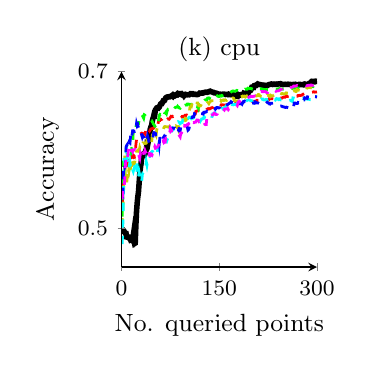
\begin{tikzpicture}

% defining custom colors
\definecolor{mycolor1}{rgb}{0.8,0.8,0}
\definecolor{mycolor2}{rgb}{0,1,1}
\definecolor{mycolor3}{rgb}{1,0,1}


\begin{axis}[
footnotesize,
width= 1.6in,
height= 1.6in,
xmin=0, xmax=300,
ymin=0.45, ymax=0.7,
ytick={0.5,0.7},
xtick = {0,150,300},
xlabel = {No. queried points},
ylabel = {Accuracy},
title = {(k) cpu},
axis on top,
axis y line = left,
axis x line = bottom
%legend entries={$optimal$,$rand$,$IVM$,$maxent$,$QBC2$,$QBC100$,$SVM$},
 %egend style={nodes=right}
]

\addplot [
color=black,
solid,
line width=2.0pt
]
coordinates{ (1,0.499527) (2,0.496581) (3,0.496832) (4,0.495753) (5,0.494346) (6,0.492938) (7,0.492908) (8,0.488359) (9,0.488206) (10,0.488063) (11,0.488077) (12,0.486814) (13,0.486628) (14,0.484573) (15,0.484872) (16,0.485447) (17,0.484227) (18,0.490009) (19,0.483911) (20,0.48008) (21,0.480615) (22,0.503247) (23,0.520835) (24,0.531765) (25,0.539852) (26,0.546142) (27,0.557429) (28,0.56957) (29,0.577113) (30,0.582536) (31,0.590636) (32,0.593758) (33,0.594381) (34,0.592747) (35,0.592676) (36,0.594642) (37,0.598584) (38,0.599647) (39,0.60655) (40,0.605852) (41,0.610446) (42,0.615498) (43,0.619219) (44,0.626236) (45,0.628912) (46,0.628997) (47,0.635925) (48,0.63941) (49,0.641944) (50,0.645492) (51,0.644958) (52,0.651003) (53,0.652204) (54,0.653492) (55,0.653568) (56,0.654178) (57,0.653669) (58,0.654604) (59,0.656877) (60,0.658615) (61,0.65929) (62,0.659189) (63,0.660764) (64,0.662477) (65,0.662426) (66,0.663015) (67,0.665152) (68,0.666605) (69,0.667059) (70,0.667461) (71,0.667314) (72,0.667673) (73,0.667952) (74,0.667756) (75,0.668267) (76,0.668306) (77,0.669138) (78,0.669724) (79,0.668801) (80,0.670061) (81,0.669528) (82,0.669082) (83,0.669577) (84,0.669773) (85,0.670852) (86,0.671677) (87,0.671077) (88,0.671928) (89,0.671892) (90,0.67191) (91,0.671237) (92,0.671571) (93,0.67057) (94,0.670824) (95,0.67067) (96,0.669318) (97,0.670356) (98,0.670855) (99,0.670514) (100,0.670294) (101,0.670207) (102,0.670381) (103,0.670418) (104,0.670379) (105,0.67089) (106,0.671683) (107,0.671656) (108,0.671537) (109,0.671637) (110,0.670902) (111,0.67082) (112,0.671069) (113,0.671025) (114,0.670913) (115,0.670531) (116,0.670531) (117,0.670743) (118,0.671032) (119,0.671627) (120,0.672445) (121,0.672303) (122,0.672506) (123,0.672487) (124,0.672787) (125,0.672549) (126,0.672781) (127,0.673218) (128,0.673541) (129,0.673792) (130,0.67371) (131,0.673546) (132,0.673564) (133,0.673991) (134,0.674125) (135,0.674684) (136,0.674935) (137,0.674413) (138,0.674159) (139,0.673956) (140,0.673566) (141,0.673531) (142,0.672884) (143,0.672794) (144,0.672602) (145,0.672531) (146,0.672008) (147,0.671903) (148,0.671576) (149,0.671188) (150,0.670539) (151,0.670832) (152,0.671038) (153,0.670861) (154,0.670836) (155,0.67101) (156,0.671046) (157,0.671072) (158,0.671076) (159,0.670882) (160,0.670698) (161,0.670789) (162,0.670884) (163,0.670605) (164,0.671023) (165,0.670484) (166,0.670432) (167,0.670938) (168,0.671058) (169,0.670591) (170,0.670365) (171,0.669918) (172,0.670086) (173,0.669327) (174,0.669494) (175,0.668853) (176,0.668671) (177,0.66873) (178,0.668506) (179,0.670752) (180,0.670358) (181,0.66999) (182,0.670063) (183,0.669848) (184,0.670465) (185,0.670208) (186,0.670041) (187,0.67005) (188,0.672211) (189,0.671935) (190,0.671762) (191,0.672054) (192,0.671639) (193,0.673613) (194,0.673699) (195,0.673534) (196,0.675219) (197,0.675518) (198,0.675819) (199,0.677423) (200,0.680117) (201,0.680304) (202,0.680204) (203,0.680005) (204,0.682142) (205,0.682389) (206,0.682372) (207,0.682419) (208,0.683495) (209,0.68417) (210,0.683765) (211,0.683579) (212,0.683516) (213,0.683308) (214,0.683091) (215,0.682803) (216,0.682625) (217,0.682774) (218,0.682548) (219,0.682088) (220,0.682377) (221,0.682061) (222,0.682225) (223,0.682254) (224,0.682277) (225,0.682891) (226,0.683356) (227,0.683516) (228,0.683524) (229,0.683874) (230,0.684128) (231,0.683782) (232,0.683514) (233,0.683706) (234,0.683984) (235,0.683747) (236,0.683796) (237,0.683868) (238,0.684023) (239,0.683774) (240,0.68405) (241,0.684315) (242,0.684298) (243,0.684261) (244,0.684487) (245,0.683976) (246,0.683955) (247,0.683726) (248,0.683468) (249,0.683723) (250,0.683666) (251,0.683792) (252,0.683718) (253,0.683652) (254,0.683711) (255,0.683802) (256,0.683784) (257,0.683605) (258,0.683584) (259,0.683286) (260,0.683446) (261,0.683298) (262,0.683113) (263,0.683457) (264,0.683597) (265,0.683456) (266,0.683384) (267,0.683636) (268,0.683231) (269,0.683143) (270,0.68295) (271,0.683014) (272,0.683439) (273,0.683242) (274,0.68356) (275,0.683465) (276,0.68328) (277,0.683423) (278,0.683372) (279,0.683161) (280,0.683909) (281,0.684077) (282,0.683718) (283,0.683311) (284,0.683207) (285,0.683405) (286,0.683932) (287,0.683882) (288,0.684792) (289,0.684964) (290,0.685719) (291,0.686763) (292,0.687456) (293,0.687306) (294,0.687346) (295,0.68701) (296,0.686903) (297,0.687641) (298,0.687757) (299,0.687492) (300,0.687736)
};

\addplot [
color=red,
dashed,
line width=1.0pt
]
coordinates{ (1,0.528765) (2,0.54206) (3,0.560389) (4,0.565016) (5,0.558062) (6,0.570054) (7,0.575923) (8,0.579584) (9,0.585579) (10,0.587453) (11,0.591187) (12,0.593199) (13,0.594671) (14,0.593046) (15,0.595236) (16,0.590511) (17,0.591041) (18,0.590416) (19,0.592274) (20,0.591277) (21,0.594764) (22,0.606095) (23,0.613168) (24,0.615037) (25,0.61501) (26,0.615351) (27,0.616037) (28,0.620201) (29,0.62009) (30,0.620782) (31,0.621285) (32,0.62088) (33,0.620376) (34,0.620352) (35,0.620867) (36,0.62005) (37,0.624454) (38,0.625134) (39,0.625975) (40,0.622106) (41,0.624221) (42,0.62495) (43,0.623885) (44,0.625338) (45,0.626547) (46,0.627009) (47,0.627077) (48,0.627602) (49,0.627617) (50,0.62868) (51,0.626474) (52,0.627906) (53,0.630034) (54,0.632859) (55,0.631926) (56,0.632665) (57,0.638092) (58,0.63768) (59,0.637536) (60,0.639091) (61,0.638728) (62,0.638976) (63,0.640845) (64,0.641424) (65,0.640697) (66,0.640811) (67,0.638396) (68,0.637916) (69,0.637661) (70,0.638639) (71,0.63948) (72,0.639192) (73,0.638987) (74,0.640061) (75,0.6415) (76,0.642766) (77,0.642419) (78,0.64284) (79,0.642311) (80,0.642735) (81,0.642321) (82,0.641868) (83,0.641649) (84,0.641144) (85,0.641378) (86,0.640877) (87,0.641123) (88,0.640695) (89,0.640476) (90,0.640825) (91,0.64061) (92,0.641265) (93,0.642612) (94,0.642781) (95,0.642408) (96,0.642783) (97,0.643645) (98,0.642915) (99,0.644305) (100,0.644519) (101,0.643889) (102,0.643483) (103,0.643583) (104,0.643241) (105,0.642293) (106,0.642444) (107,0.642624) (108,0.642758) (109,0.642712) (110,0.642731) (111,0.643052) (112,0.644942) (113,0.64534) (114,0.649014) (115,0.649482) (116,0.649699) (117,0.649747) (118,0.65043) (119,0.650879) (120,0.651025) (121,0.650924) (122,0.651362) (123,0.651042) (124,0.651123) (125,0.651105) (126,0.650594) (127,0.651151) (128,0.650892) (129,0.650272) (130,0.650157) (131,0.651845) (132,0.651755) (133,0.652622) (134,0.652022) (135,0.652028) (136,0.652839) (137,0.652943) (138,0.653736) (139,0.653846) (140,0.654041) (141,0.65522) (142,0.655021) (143,0.655153) (144,0.656206) (145,0.65656) (146,0.655837) (147,0.655673) (148,0.65617) (149,0.65595) (150,0.656235) (151,0.655711) (152,0.655672) (153,0.657509) (154,0.657696) (155,0.657639) (156,0.657356) (157,0.657235) (158,0.657026) (159,0.65719) (160,0.657275) (161,0.657628) (162,0.657734) (163,0.657694) (164,0.658127) (165,0.658784) (166,0.658598) (167,0.659037) (168,0.658857) (169,0.659079) (170,0.659011) (171,0.658989) (172,0.658614) (173,0.658441) (174,0.659071) (175,0.660054) (176,0.660129) (177,0.659915) (178,0.65993) (179,0.659531) (180,0.659496) (181,0.659341) (182,0.659258) (183,0.659389) (184,0.659282) (185,0.659688) (186,0.660107) (187,0.660059) (188,0.660159) (189,0.660166) (190,0.660153) (191,0.660611) (192,0.65999) (193,0.660366) (194,0.66045) (195,0.660608) (196,0.660989) (197,0.661158) (198,0.662031) (199,0.662172) (200,0.662069) (201,0.661964) (202,0.661815) (203,0.661652) (204,0.661488) (205,0.661497) (206,0.662456) (207,0.662411) (208,0.663217) (209,0.663118) (210,0.663076) (211,0.66316) (212,0.663298) (213,0.663892) (214,0.663621) (215,0.663976) (216,0.663979) (217,0.664066) (218,0.663994) (219,0.664001) (220,0.663355) (221,0.663772) (222,0.663304) (223,0.663438) (224,0.663181) (225,0.663112) (226,0.663657) (227,0.665458) (228,0.665435) (229,0.665201) (230,0.665221) (231,0.665166) (232,0.665176) (233,0.665085) (234,0.664966) (235,0.66497) (236,0.66539) (237,0.665427) (238,0.665336) (239,0.665439) (240,0.665376) (241,0.665436) (242,0.665408) (243,0.665192) (244,0.665177) (245,0.666148) (246,0.66605) (247,0.666706) (248,0.666994) (249,0.667421) (250,0.66719) (251,0.667194) (252,0.668349) (253,0.668277) (254,0.668229) (255,0.668248) (256,0.668442) (257,0.668735) (258,0.668781) (259,0.6688) (260,0.668496) (261,0.668466) (262,0.668485) (263,0.66828) (264,0.668379) (265,0.66833) (266,0.668265) (267,0.668242) (268,0.66841) (269,0.668627) (270,0.668475) (271,0.669482) (272,0.669446) (273,0.669585) (274,0.669483) (275,0.66955) (276,0.669597) (277,0.669873) (278,0.670868) (279,0.671108) (280,0.671656) (281,0.672096) (282,0.672601) (283,0.672855) (284,0.673198) (285,0.673197) (286,0.6734) (287,0.673406) (288,0.673345) (289,0.673279) (290,0.673446) (291,0.673249) (292,0.673544) (293,0.673704) (294,0.673905) (295,0.674184) (296,0.673733) (297,0.67372) (298,0.673818) (299,0.673823) (300,0.673923)
};

\addplot [
color=green,
dashed,
line width=1.0pt
]
coordinates{ (1,0.514441) (2,0.547796) (3,0.583818) (4,0.58362) (5,0.592509) (6,0.592708) (7,0.599063) (8,0.596707) (9,0.597032) (10,0.586075) (11,0.582064) (12,0.576249) (13,0.580966) (14,0.593211) (15,0.596161) (16,0.605055) (17,0.604738) (18,0.623986) (19,0.624433) (20,0.62878) (21,0.626838) (22,0.628912) (23,0.632552) (24,0.633727) (25,0.632882) (26,0.633079) (27,0.637825) (28,0.642277) (29,0.644661) (30,0.644759) (31,0.644816) (32,0.643748) (33,0.642043) (34,0.640421) (35,0.644642) (36,0.644132) (37,0.64244) (38,0.641878) (39,0.641488) (40,0.64022) (41,0.638823) (42,0.638103) (43,0.638424) (44,0.637811) (45,0.637831) (46,0.637544) (47,0.636075) (48,0.634582) (49,0.632765) (50,0.632144) (51,0.630268) (52,0.629278) (53,0.628359) (54,0.628331) (55,0.628309) (56,0.635287) (57,0.638437) (58,0.644216) (59,0.645361) (60,0.644921) (61,0.645169) (62,0.643668) (63,0.643004) (64,0.64159) (65,0.64101) (66,0.646239) (67,0.646571) (68,0.647929) (69,0.646367) (70,0.649597) (71,0.651236) (72,0.650588) (73,0.651733) (74,0.651602) (75,0.65358) (76,0.654065) (77,0.653861) (78,0.653245) (79,0.653034) (80,0.652862) (81,0.652478) (82,0.65384) (83,0.654464) (84,0.654518) (85,0.654389) (86,0.655604) (87,0.654488) (88,0.654274) (89,0.653258) (90,0.653066) (91,0.654562) (92,0.654116) (93,0.658098) (94,0.658913) (95,0.657744) (96,0.657169) (97,0.656824) (98,0.657245) (99,0.657342) (100,0.657193) (101,0.65852) (102,0.658517) (103,0.658458) (104,0.657999) (105,0.657487) (106,0.657234) (107,0.658085) (108,0.658136) (109,0.657631) (110,0.655206) (111,0.655041) (112,0.65536) (113,0.655081) (114,0.652826) (115,0.653001) (116,0.6525) (117,0.655675) (118,0.653525) (119,0.657669) (120,0.657358) (121,0.661395) (122,0.661639) (123,0.66122) (124,0.661923) (125,0.663256) (126,0.663779) (127,0.662957) (128,0.663692) (129,0.663922) (130,0.663935) (131,0.663574) (132,0.666046) (133,0.666179) (134,0.66636) (135,0.665816) (136,0.667903) (137,0.667635) (138,0.667546) (139,0.667356) (140,0.666898) (141,0.666319) (142,0.665806) (143,0.666322) (144,0.668582) (145,0.668214) (146,0.668729) (147,0.669047) (148,0.668345) (149,0.668268) (150,0.668123) (151,0.668934) (152,0.668941) (153,0.668712) (154,0.669484) (155,0.669044) (156,0.669041) (157,0.669356) (158,0.669367) (159,0.669798) (160,0.669854) (161,0.670846) (162,0.670824) (163,0.671588) (164,0.671523) (165,0.671973) (166,0.671824) (167,0.672701) (168,0.673593) (169,0.674595) (170,0.674988) (171,0.675283) (172,0.675058) (173,0.674717) (174,0.674726) (175,0.67516) (176,0.675506) (177,0.675962) (178,0.675793) (179,0.675511) (180,0.675696) (181,0.675536) (182,0.675732) (183,0.675659) (184,0.675592) (185,0.675516) (186,0.67671) (187,0.676706) (188,0.676715) (189,0.676413) (190,0.677506) (191,0.677325) (192,0.677573) (193,0.677497) (194,0.678781) (195,0.678717) (196,0.678567) (197,0.67837) (198,0.678501) (199,0.678298) (200,0.677988) (201,0.677428) (202,0.677328) (203,0.676963) (204,0.677734) (205,0.677664) (206,0.678026) (207,0.678087) (208,0.677952) (209,0.679136) (210,0.678689) (211,0.678553) (212,0.678243) (213,0.678112) (214,0.677951) (215,0.677913) (216,0.677672) (217,0.677469) (218,0.677223) (219,0.677151) (220,0.676959) (221,0.676993) (222,0.676618) (223,0.676663) (224,0.677214) (225,0.677148) (226,0.678126) (227,0.677872) (228,0.677821) (229,0.677645) (230,0.677625) (231,0.677729) (232,0.677755) (233,0.677878) (234,0.677957) (235,0.67788) (236,0.677781) (237,0.677638) (238,0.677828) (239,0.677768) (240,0.677498) (241,0.677459) (242,0.678254) (243,0.678166) (244,0.677854) (245,0.677817) (246,0.677635) (247,0.677823) (248,0.677514) (249,0.67749) (250,0.677498) (251,0.677447) (252,0.677585) (253,0.677487) (254,0.6774) (255,0.677311) (256,0.677262) (257,0.677431) (258,0.677745) (259,0.677848) (260,0.677593) (261,0.678578) (262,0.678352) (263,0.679232) (264,0.679096) (265,0.678695) (266,0.678792) (267,0.678908) (268,0.678938) (269,0.678815) (270,0.678815) (271,0.678629) (272,0.678991) (273,0.678893) (274,0.678858) (275,0.678741) (276,0.678727) (277,0.678381) (278,0.678198) (279,0.67813) (280,0.677772) (281,0.679387) (282,0.67934) (283,0.679289) (284,0.679204) (285,0.680826) (286,0.680573) (287,0.680574) (288,0.680259) (289,0.680945) (290,0.680605) (291,0.680484) (292,0.680484) (293,0.680889) (294,0.68077) (295,0.681618) (296,0.681426) (297,0.681228) (298,0.680917) (299,0.680792) (300,0.680688)
};

\addplot [
color=mycolor1,
dashed,
line width=1.0pt
]
coordinates{ (1,0.501807) (2,0.521194) (3,0.54198) (4,0.574652) (5,0.592374) (6,0.560589) (7,0.560887) (8,0.557566) (9,0.568816) (10,0.576467) (11,0.572788) (12,0.579093) (13,0.578443) (14,0.577725) (15,0.587256) (16,0.585856) (17,0.582934) (18,0.58075) (19,0.581313) (20,0.582758) (21,0.587508) (22,0.591187) (23,0.59757) (24,0.598441) (25,0.599297) (26,0.598361) (27,0.598901) (28,0.602905) (29,0.600448) (30,0.602127) (31,0.605506) (32,0.605976) (33,0.608812) (34,0.608753) (35,0.607991) (36,0.608447) (37,0.608134) (38,0.608514) (39,0.611685) (40,0.613248) (41,0.613831) (42,0.613144) (43,0.612386) (44,0.608661) (45,0.607624) (46,0.608629) (47,0.616221) (48,0.624222) (49,0.621324) (50,0.619824) (51,0.619881) (52,0.620641) (53,0.618781) (54,0.625401) (55,0.627919) (56,0.627182) (57,0.626944) (58,0.627006) (59,0.627417) (60,0.627458) (61,0.626514) (62,0.625273) (63,0.625715) (64,0.625859) (65,0.62839) (66,0.6296) (67,0.629642) (68,0.629396) (69,0.62941) (70,0.629302) (71,0.62923) (72,0.629145) (73,0.629363) (74,0.630185) (75,0.629572) (76,0.627497) (77,0.627617) (78,0.629162) (79,0.629524) (80,0.628899) (81,0.629105) (82,0.630136) (83,0.630583) (84,0.629484) (85,0.628777) (86,0.628938) (87,0.626613) (88,0.632075) (89,0.631466) (90,0.631157) (91,0.633359) (92,0.63349) (93,0.637409) (94,0.638539) (95,0.638315) (96,0.638132) (97,0.639391) (98,0.637395) (99,0.637785) (100,0.639292) (101,0.641195) (102,0.640947) (103,0.64487) (104,0.647519) (105,0.65446) (106,0.654915) (107,0.654775) (108,0.658211) (109,0.66042) (110,0.661341) (111,0.66108) (112,0.659808) (113,0.660528) (114,0.657549) (115,0.658112) (116,0.659876) (117,0.659895) (118,0.656884) (119,0.656131) (120,0.65611) (121,0.656058) (122,0.656986) (123,0.659228) (124,0.6589) (125,0.657451) (126,0.657728) (127,0.657833) (128,0.658209) (129,0.657433) (130,0.658001) (131,0.658599) (132,0.660307) (133,0.660234) (134,0.659089) (135,0.660703) (136,0.661321) (137,0.662412) (138,0.662696) (139,0.66272) (140,0.662602) (141,0.662529) (142,0.662238) (143,0.661776) (144,0.662334) (145,0.66191) (146,0.662279) (147,0.663109) (148,0.663) (149,0.663249) (150,0.662597) (151,0.662134) (152,0.663083) (153,0.662054) (154,0.662898) (155,0.66347) (156,0.663726) (157,0.6629) (158,0.663185) (159,0.663828) (160,0.663315) (161,0.663153) (162,0.66344) (163,0.664434) (164,0.664372) (165,0.665128) (166,0.664921) (167,0.665496) (168,0.663187) (169,0.664873) (170,0.665853) (171,0.666223) (172,0.665815) (173,0.662961) (174,0.663014) (175,0.662674) (176,0.662316) (177,0.662411) (178,0.660143) (179,0.66365) (180,0.663646) (181,0.66702) (182,0.668053) (183,0.667577) (184,0.667944) (185,0.667646) (186,0.668563) (187,0.66819) (188,0.668584) (189,0.667795) (190,0.667412) (191,0.668401) (192,0.669004) (193,0.668715) (194,0.668503) (195,0.66863) (196,0.668729) (197,0.668787) (198,0.670476) (199,0.670687) (200,0.670324) (201,0.669911) (202,0.669904) (203,0.669921) (204,0.669326) (205,0.669122) (206,0.669026) (207,0.668799) (208,0.669017) (209,0.669254) (210,0.670674) (211,0.670536) (212,0.668933) (213,0.668887) (214,0.668173) (215,0.668081) (216,0.668288) (217,0.667754) (218,0.667453) (219,0.666149) (220,0.666481) (221,0.667802) (222,0.66734) (223,0.667694) (224,0.669723) (225,0.669389) (226,0.669161) (227,0.66958) (228,0.668255) (229,0.669538) (230,0.668873) (231,0.669197) (232,0.669108) (233,0.669345) (234,0.669879) (235,0.672627) (236,0.672425) (237,0.672899) (238,0.672957) (239,0.672715) (240,0.672548) (241,0.672781) (242,0.672793) (243,0.672558) (244,0.672496) (245,0.67183) (246,0.671491) (247,0.671846) (248,0.671752) (249,0.671356) (250,0.671709) (251,0.671566) (252,0.672129) (253,0.672087) (254,0.67689) (255,0.67642) (256,0.676489) (257,0.676135) (258,0.675858) (259,0.675471) (260,0.675285) (261,0.675279) (262,0.67516) (263,0.675) (264,0.675405) (265,0.675269) (266,0.675132) (267,0.674619) (268,0.674589) (269,0.677071) (270,0.676782) (271,0.676519) (272,0.676157) (273,0.675908) (274,0.675644) (275,0.675687) (276,0.676906) (277,0.677551) (278,0.677499) (279,0.677392) (280,0.677569) (281,0.677155) (282,0.677089) (283,0.677004) (284,0.676668) (285,0.68021) (286,0.679722) (287,0.679668) (288,0.67963) (289,0.679621) (290,0.679409) (291,0.681801) (292,0.681598) (293,0.681319) (294,0.681671) (295,0.681574) (296,0.68142) (297,0.681054) (298,0.680917) (299,0.680821) (300,0.680473)
};

\addplot [
color=mycolor2,
dashed,
line width=1.0pt
]
coordinates{ (1,0.479234) (2,0.503261) (3,0.542935) (4,0.589311) (5,0.584032) (6,0.588865) (7,0.598279) (8,0.606129) (9,0.585457) (10,0.582916) (11,0.575869) (12,0.578577) (13,0.583567) (14,0.57722) (15,0.573357) (16,0.571869) (17,0.57468) (18,0.572295) (19,0.575425) (20,0.577585) (21,0.581434) (22,0.586466) (23,0.584939) (24,0.571036) (25,0.571946) (26,0.564865) (27,0.571315) (28,0.567005) (29,0.55815) (30,0.559136) (31,0.560019) (32,0.568428) (33,0.570689) (34,0.570738) (35,0.571718) (36,0.575925) (37,0.576662) (38,0.584459) (39,0.580364) (40,0.585216) (41,0.584915) (42,0.591423) (43,0.591284) (44,0.591818) (45,0.594949) (46,0.597212) (47,0.597998) (48,0.597614) (49,0.596489) (50,0.597358) (51,0.599017) (52,0.599519) (53,0.599179) (54,0.600125) (55,0.5967) (56,0.60536) (57,0.607119) (58,0.606246) (59,0.606481) (60,0.606814) (61,0.607884) (62,0.609819) (63,0.608825) (64,0.611618) (65,0.612268) (66,0.612983) (67,0.610487) (68,0.610658) (69,0.610196) (70,0.612676) (71,0.614781) (72,0.618292) (73,0.620013) (74,0.621047) (75,0.620224) (76,0.621693) (77,0.626805) (78,0.627552) (79,0.625519) (80,0.626279) (81,0.626967) (82,0.627231) (83,0.627046) (84,0.62792) (85,0.628929) (86,0.634423) (87,0.635899) (88,0.635478) (89,0.634659) (90,0.633368) (91,0.633983) (92,0.635028) (93,0.635018) (94,0.637634) (95,0.636976) (96,0.639702) (97,0.639991) (98,0.641385) (99,0.640954) (100,0.642421) (101,0.642056) (102,0.642292) (103,0.640761) (104,0.641617) (105,0.641362) (106,0.641455) (107,0.640224) (108,0.641289) (109,0.641129) (110,0.640605) (111,0.640985) (112,0.641928) (113,0.641855) (114,0.640828) (115,0.64041) (116,0.64082) (117,0.64005) (118,0.638424) (119,0.638376) (120,0.638457) (121,0.636767) (122,0.638176) (123,0.639453) (124,0.639351) (125,0.639699) (126,0.641021) (127,0.640681) (128,0.642868) (129,0.643327) (130,0.643403) (131,0.643248) (132,0.645433) (133,0.644489) (134,0.644289) (135,0.644788) (136,0.644609) (137,0.644139) (138,0.642774) (139,0.642595) (140,0.646109) (141,0.646235) (142,0.646287) (143,0.645808) (144,0.647423) (145,0.647302) (146,0.647495) (147,0.647183) (148,0.64751) (149,0.648001) (150,0.647421) (151,0.65103) (152,0.650923) (153,0.651157) (154,0.652506) (155,0.652301) (156,0.653098) (157,0.652211) (158,0.652088) (159,0.654233) (160,0.655426) (161,0.654025) (162,0.654072) (163,0.654845) (164,0.654422) (165,0.654851) (166,0.654756) (167,0.654262) (168,0.652892) (169,0.652722) (170,0.656636) (171,0.657746) (172,0.65777) (173,0.657829) (174,0.657859) (175,0.657897) (176,0.658247) (177,0.658992) (178,0.658784) (179,0.658882) (180,0.65862) (181,0.658929) (182,0.659039) (183,0.659719) (184,0.661344) (185,0.660737) (186,0.66063) (187,0.661436) (188,0.661858) (189,0.66145) (190,0.661738) (191,0.662362) (192,0.662805) (193,0.663301) (194,0.663684) (195,0.663723) (196,0.663539) (197,0.66354) (198,0.662607) (199,0.662612) (200,0.662537) (201,0.662487) (202,0.662233) (203,0.662745) (204,0.663053) (205,0.66349) (206,0.66365) (207,0.663236) (208,0.663299) (209,0.663648) (210,0.663589) (211,0.664018) (212,0.664056) (213,0.663602) (214,0.664126) (215,0.664956) (216,0.664635) (217,0.664803) (218,0.663796) (219,0.663716) (220,0.663669) (221,0.664213) (222,0.664363) (223,0.664446) (224,0.663572) (225,0.663562) (226,0.664419) (227,0.664254) (228,0.665794) (229,0.665821) (230,0.66473) (231,0.664858) (232,0.66479) (233,0.664392) (234,0.663666) (235,0.664087) (236,0.663646) (237,0.664795) (238,0.665521) (239,0.665185) (240,0.664667) (241,0.664229) (242,0.665143) (243,0.664636) (244,0.663973) (245,0.663726) (246,0.663632) (247,0.663411) (248,0.663324) (249,0.663752) (250,0.663564) (251,0.663545) (252,0.663443) (253,0.663575) (254,0.663091) (255,0.663338) (256,0.663009) (257,0.662889) (258,0.663179) (259,0.663264) (260,0.662663) (261,0.662339) (262,0.661958) (263,0.666297) (264,0.666086) (265,0.666071) (266,0.665786) (267,0.665712) (268,0.665756) (269,0.665525) (270,0.665558) (271,0.665751) (272,0.665419) (273,0.665154) (274,0.665458) (275,0.665161) (276,0.665184) (277,0.665552) (278,0.665614) (279,0.665366) (280,0.665097) (281,0.665159) (282,0.665055) (283,0.665016) (284,0.664944) (285,0.66472) (286,0.664692) (287,0.664706) (288,0.664498) (289,0.664214) (290,0.663994) (291,0.663997) (292,0.667149) (293,0.668961) (294,0.668907) (295,0.668808) (296,0.668753) (297,0.668612) (298,0.668167) (299,0.668069) (300,0.66799)
};

\addplot [
color=blue,
dashed,
line width=1.0pt
]
coordinates{ (1,0.544732) (2,0.54297) (3,0.573277) (4,0.581393) (5,0.577688) (6,0.580193) (7,0.603612) (8,0.605466) (9,0.606842) (10,0.604621) (11,0.602783) (12,0.609534) (13,0.608672) (14,0.61865) (15,0.613621) (16,0.618831) (17,0.624436) (18,0.624458) (19,0.623955) (20,0.621065) (21,0.624279) (22,0.626836) (23,0.633364) (24,0.630366) (25,0.631721) (26,0.627702) (27,0.628948) (28,0.625868) (29,0.622667) (30,0.62175) (31,0.61844) (32,0.61561) (33,0.617359) (34,0.616199) (35,0.615371) (36,0.611396) (37,0.612296) (38,0.611959) (39,0.611287) (40,0.61734) (41,0.614411) (42,0.609889) (43,0.607949) (44,0.609596) (45,0.610593) (46,0.611065) (47,0.613079) (48,0.615282) (49,0.620353) (50,0.62187) (51,0.621459) (52,0.620981) (53,0.619463) (54,0.620104) (55,0.618642) (56,0.618079) (57,0.615809) (58,0.608265) (59,0.617066) (60,0.616182) (61,0.615886) (62,0.612444) (63,0.611217) (64,0.615385) (65,0.616695) (66,0.614233) (67,0.618527) (68,0.62172) (69,0.622449) (70,0.624092) (71,0.62481) (72,0.626197) (73,0.626835) (74,0.627947) (75,0.626409) (76,0.625245) (77,0.624908) (78,0.627789) (79,0.627658) (80,0.62788) (81,0.627489) (82,0.627491) (83,0.626514) (84,0.629444) (85,0.62872) (86,0.623662) (87,0.623939) (88,0.626656) (89,0.626193) (90,0.624507) (91,0.629491) (92,0.629801) (93,0.629564) (94,0.628155) (95,0.627757) (96,0.628421) (97,0.62738) (98,0.627572) (99,0.627556) (100,0.629398) (101,0.628859) (102,0.625016) (103,0.625755) (104,0.628547) (105,0.633354) (106,0.634378) (107,0.635438) (108,0.640472) (109,0.642284) (110,0.642285) (111,0.642448) (112,0.646479) (113,0.646338) (114,0.647078) (115,0.647462) (116,0.647466) (117,0.648856) (118,0.650163) (119,0.649258) (120,0.649083) (121,0.648024) (122,0.646332) (123,0.646195) (124,0.646063) (125,0.645713) (126,0.647632) (127,0.647271) (128,0.648252) (129,0.648396) (130,0.648386) (131,0.649402) (132,0.649155) (133,0.648911) (134,0.648525) (135,0.649169) (136,0.65019) (137,0.651289) (138,0.650663) (139,0.650524) (140,0.650171) (141,0.649931) (142,0.650639) (143,0.650871) (144,0.652904) (145,0.652691) (146,0.654101) (147,0.654164) (148,0.654008) (149,0.653536) (150,0.653768) (151,0.653543) (152,0.652799) (153,0.653775) (154,0.654218) (155,0.654126) (156,0.654562) (157,0.654635) (158,0.654143) (159,0.653244) (160,0.654648) (161,0.655802) (162,0.657035) (163,0.658219) (164,0.658714) (165,0.659022) (166,0.659964) (167,0.660079) (168,0.661422) (169,0.660854) (170,0.660455) (171,0.660031) (172,0.659439) (173,0.659106) (174,0.658728) (175,0.658156) (176,0.657862) (177,0.657615) (178,0.65811) (179,0.660114) (180,0.659511) (181,0.658905) (182,0.658753) (183,0.659147) (184,0.659125) (185,0.658313) (186,0.660107) (187,0.661585) (188,0.661252) (189,0.662027) (190,0.660938) (191,0.659938) (192,0.659703) (193,0.659244) (194,0.659679) (195,0.659444) (196,0.659698) (197,0.659175) (198,0.658907) (199,0.659209) (200,0.65988) (201,0.659844) (202,0.659614) (203,0.659733) (204,0.659464) (205,0.661127) (206,0.660401) (207,0.660595) (208,0.659816) (209,0.659859) (210,0.659685) (211,0.659312) (212,0.659485) (213,0.659925) (214,0.661274) (215,0.661516) (216,0.660974) (217,0.661206) (218,0.661667) (219,0.661818) (220,0.662239) (221,0.662117) (222,0.661931) (223,0.661046) (224,0.660331) (225,0.659658) (226,0.659552) (227,0.658524) (228,0.658336) (229,0.659421) (230,0.659469) (231,0.659356) (232,0.659368) (233,0.65947) (234,0.658805) (235,0.658944) (236,0.658476) (237,0.658415) (238,0.658263) (239,0.657497) (240,0.657081) (241,0.656351) (242,0.656075) (243,0.655739) (244,0.65595) (245,0.655881) (246,0.655668) (247,0.655027) (248,0.654875) (249,0.654882) (250,0.654333) (251,0.654216) (252,0.654208) (253,0.654541) (254,0.654277) (255,0.653918) (256,0.653593) (257,0.65356) (258,0.654039) (259,0.653607) (260,0.656261) (261,0.655784) (262,0.655685) (263,0.65552) (264,0.654721) (265,0.659653) (266,0.659643) (267,0.659649) (268,0.659287) (269,0.659218) (270,0.659173) (271,0.660501) (272,0.660122) (273,0.659517) (274,0.664227) (275,0.664266) (276,0.664482) (277,0.664424) (278,0.664199) (279,0.663825) (280,0.663736) (281,0.666502) (282,0.666189) (283,0.665991) (284,0.665756) (285,0.66561) (286,0.670428) (287,0.670097) (288,0.670002) (289,0.669909) (290,0.669771) (291,0.669355) (292,0.668887) (293,0.668576) (294,0.668316) (295,0.66811) (296,0.668079) (297,0.66801) (298,0.667915) (299,0.667595) (300,0.667485)
};

\addplot [
color=mycolor3,
dashed,
line width=1.0pt
]
coordinates{ (1,0.536743) (2,0.547781) (3,0.546634) (4,0.551618) (5,0.562681) (6,0.581311) (7,0.589086) (8,0.58954) (9,0.586292) (10,0.595638) (11,0.602901) (12,0.606068) (13,0.60176) (14,0.601054) (15,0.599054) (16,0.59933) (17,0.597537) (18,0.599821) (19,0.599575) (20,0.600186) (21,0.600499) (22,0.599109) (23,0.600237) (24,0.598774) (25,0.598492) (26,0.594845) (27,0.591589) (28,0.589159) (29,0.595207) (30,0.59323) (31,0.596004) (32,0.596112) (33,0.59945) (34,0.595317) (35,0.595487) (36,0.598794) (37,0.596586) (38,0.59483) (39,0.593763) (40,0.594396) (41,0.594584) (42,0.599182) (43,0.592719) (44,0.592414) (45,0.594184) (46,0.594546) (47,0.593534) (48,0.596065) (49,0.602498) (50,0.601787) (51,0.603966) (52,0.601833) (53,0.60221) (54,0.603094) (55,0.603627) (56,0.604601) (57,0.606591) (58,0.609651) (59,0.608895) (60,0.611917) (61,0.611912) (62,0.611302) (63,0.609779) (64,0.611189) (65,0.609156) (66,0.609997) (67,0.609864) (68,0.614344) (69,0.613951) (70,0.616503) (71,0.617533) (72,0.617147) (73,0.622204) (74,0.622341) (75,0.627407) (76,0.625911) (77,0.62443) (78,0.624938) (79,0.625213) (80,0.624638) (81,0.622344) (82,0.621849) (83,0.621679) (84,0.621282) (85,0.621282) (86,0.621262) (87,0.619882) (88,0.618758) (89,0.617851) (90,0.616526) (91,0.621135) (92,0.621388) (93,0.62389) (94,0.622729) (95,0.622926) (96,0.622099) (97,0.630917) (98,0.630604) (99,0.631062) (100,0.631453) (101,0.632231) (102,0.631981) (103,0.633518) (104,0.634029) (105,0.634619) (106,0.633171) (107,0.632214) (108,0.630369) (109,0.63496) (110,0.634978) (111,0.634641) (112,0.6349) (113,0.635427) (114,0.635442) (115,0.637347) (116,0.638162) (117,0.638056) (118,0.63781) (119,0.63625) (120,0.637028) (121,0.635426) (122,0.635323) (123,0.636838) (124,0.634996) (125,0.634165) (126,0.633709) (127,0.6342) (128,0.632508) (129,0.632146) (130,0.632207) (131,0.641653) (132,0.642627) (133,0.641872) (134,0.641515) (135,0.644018) (136,0.644094) (137,0.644046) (138,0.644576) (139,0.644518) (140,0.644544) (141,0.645672) (142,0.646808) (143,0.646442) (144,0.645555) (145,0.645076) (146,0.645104) (147,0.645777) (148,0.648224) (149,0.648203) (150,0.647305) (151,0.646954) (152,0.647019) (153,0.647518) (154,0.647841) (155,0.649005) (156,0.648717) (157,0.649497) (158,0.651897) (159,0.652222) (160,0.652035) (161,0.652019) (162,0.652253) (163,0.652987) (164,0.651331) (165,0.652259) (166,0.652806) (167,0.653328) (168,0.653329) (169,0.653217) (170,0.653551) (171,0.653866) (172,0.653877) (173,0.654311) (174,0.654238) (175,0.654499) (176,0.654851) (177,0.654975) (178,0.657242) (179,0.661209) (180,0.661537) (181,0.661181) (182,0.66251) (183,0.663607) (184,0.663518) (185,0.663574) (186,0.664009) (187,0.664565) (188,0.664796) (189,0.665428) (190,0.665602) (191,0.665566) (192,0.665532) (193,0.66655) (194,0.66692) (195,0.667021) (196,0.667462) (197,0.668011) (198,0.667897) (199,0.668083) (200,0.668432) (201,0.668006) (202,0.668155) (203,0.668421) (204,0.668572) (205,0.668879) (206,0.668671) (207,0.669105) (208,0.669951) (209,0.673754) (210,0.673802) (211,0.673958) (212,0.674256) (213,0.673991) (214,0.674499) (215,0.674453) (216,0.674371) (217,0.674168) (218,0.674158) (219,0.674552) (220,0.674402) (221,0.674155) (222,0.674183) (223,0.672891) (224,0.672891) (225,0.674337) (226,0.674373) (227,0.673923) (228,0.673939) (229,0.673764) (230,0.673481) (231,0.674112) (232,0.674118) (233,0.675295) (234,0.675348) (235,0.675365) (236,0.675442) (237,0.674753) (238,0.67516) (239,0.675301) (240,0.675457) (241,0.675375) (242,0.675918) (243,0.676192) (244,0.67741) (245,0.677397) (246,0.677512) (247,0.678065) (248,0.679588) (249,0.679413) (250,0.679353) (251,0.679279) (252,0.679792) (253,0.679953) (254,0.679962) (255,0.679996) (256,0.679739) (257,0.679697) (258,0.679913) (259,0.680092) (260,0.68008) (261,0.680071) (262,0.679885) (263,0.680197) (264,0.681457) (265,0.681448) (266,0.681425) (267,0.681355) (268,0.681509) (269,0.682084) (270,0.682271) (271,0.681804) (272,0.681848) (273,0.681883) (274,0.681886) (275,0.681923) (276,0.6823) (277,0.682043) (278,0.6821) (279,0.682058) (280,0.682068) (281,0.681952) (282,0.682067) (283,0.681767) (284,0.681734) (285,0.682076) (286,0.682126) (287,0.682457) (288,0.682605) (289,0.682457) (290,0.682691) (291,0.682675) (292,0.682676) (293,0.682551) (294,0.68233) (295,0.682679) (296,0.682787) (297,0.682659) (298,0.683006) (299,0.682961) (300,0.683)
};

\end{axis}
\end{tikzpicture}
&
% This file was created by matlab2tikz v0.0.7.
% Copyright (c) 2008--2010, Nico Schlömer <nico.schloemer@gmail.com>
% All rights reserved.
% 
% The latest updates can be retrieved from
%   http://www.mathworks.com/matlabcentral/fileexchange/22022-matlab2tikz
% where you can also make suggestions and rate matlab2tikz.
% 
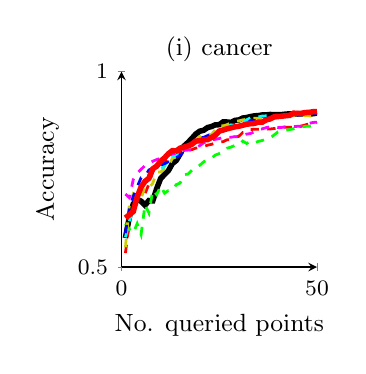
\begin{tikzpicture}

% defining custom colors
\definecolor{mycolor1}{rgb}{0.8,0.8,0}
\definecolor{mycolor2}{rgb}{0,1,1}
\definecolor{mycolor3}{rgb}{1,0,1}


\begin{axis}[
footnotesize,
width= 1.6in,
height= 1.6in,
xmin=0, xmax=50,
ymin=0.5, ymax=1,
ytick={0.5,1},
xtick = {0,50},
xlabel = {No. queried points},
ylabel = {Accuracy},
title = {(i) cancer},
axis on top,
axis y line = left,
axis x line = bottom
%legend entries={$optimal$,$rand$,$IVM$,$maxent$,$QBC2$,$QBC100$,$SVM$},
 %egend style={nodes=right}
]
\addplot [
color=black,
solid,
line width=2.0pt
]
coordinates{ (1,0.574217) (2,0.62793) (3,0.661375) (4,0.673038) (5,0.668567) (6,0.658111) (7,0.670141) (8,0.669476) (9,0.7008) (10,0.726428) (11,0.736711) (12,0.746786) (13,0.764648) (14,0.772589) (15,0.789539) (16,0.809629) (17,0.818582) (18,0.829098) (19,0.840272) (20,0.847444) (21,0.849872) (22,0.856744) (23,0.859344) (24,0.863751) (25,0.864085) (26,0.871329) (27,0.870972) (28,0.869895) (29,0.875048) (30,0.87634) (31,0.881149) (32,0.882478) (33,0.884911) (34,0.886762) (35,0.887407) (36,0.889089) (37,0.889162) (38,0.890223) (39,0.890013) (40,0.889872) (41,0.890051) (42,0.891106) (43,0.892024) (44,0.89149) (45,0.892205) (46,0.891623) (47,0.891595) (48,0.89155) (49,0.892287) (50,0.894004)
};

\addplot [
color=red,
dashed,
line width=1.0pt
]
coordinates{ (1,0.535742) (2,0.616989) (3,0.660018) (4,0.671112) (5,0.684063) (6,0.687282) (7,0.71214) (8,0.745198) (9,0.752483) (10,0.756891) (11,0.76958) (12,0.773514) (13,0.781026) (14,0.785675) (15,0.793858) (16,0.795764) (17,0.799084) (18,0.800403) (19,0.804281) (20,0.805622) (21,0.808194) (22,0.811788) (23,0.813825) (24,0.817551) (25,0.819387) (26,0.82081) (27,0.825565) (28,0.825811) (29,0.832864) (30,0.834297) (31,0.844102) (32,0.844271) (33,0.851679) (34,0.852512) (35,0.85251) (36,0.852034) (37,0.85259) (38,0.853108) (39,0.854254) (40,0.855329) (41,0.857922) (42,0.857842) (43,0.857285) (44,0.857612) (45,0.859041) (46,0.860755) (47,0.863558) (48,0.866195) (49,0.869403) (50,0.869687)
};

\addplot [
color=green,
dashed,
line width=1.0pt
]
coordinates{ (1,0.610781) (2,0.59652) (3,0.587019) (4,0.610981) (5,0.583353) (6,0.65952) (7,0.638415) (8,0.696562) (9,0.68523) (10,0.707412) (11,0.689023) (12,0.695586) (13,0.696924) (14,0.710825) (15,0.714953) (16,0.736302) (17,0.737904) (18,0.747824) (19,0.753162) (20,0.760132) (21,0.769101) (22,0.773976) (23,0.7785) (24,0.786485) (25,0.790238) (26,0.79456) (27,0.803962) (28,0.806901) (29,0.811154) (30,0.812271) (31,0.822222) (32,0.816165) (33,0.82139) (34,0.817514) (35,0.821509) (36,0.823719) (37,0.827412) (38,0.830023) (39,0.83758) (40,0.845696) (41,0.847051) (42,0.849592) (43,0.851698) (44,0.853657) (45,0.856296) (46,0.857964) (47,0.85982) (48,0.860201) (49,0.861967) (50,0.863434)
};

\addplot [
color=mycolor1,
dashed,
line width=1.0pt
]
coordinates{ (1,0.550928) (2,0.659257) (3,0.687257) (4,0.677099) (5,0.674766) (6,0.706) (7,0.70335) (8,0.714109) (9,0.743103) (10,0.743255) (11,0.751388) (12,0.758453) (13,0.7779) (14,0.781788) (15,0.794995) (16,0.798309) (17,0.806485) (18,0.813159) (19,0.825249) (20,0.833789) (21,0.837481) (22,0.839234) (23,0.838422) (24,0.851552) (25,0.861868) (26,0.861221) (27,0.86416) (28,0.86898) (29,0.872372) (30,0.873973) (31,0.876427) (32,0.877794) (33,0.879112) (34,0.880571) (35,0.880227) (36,0.880456) (37,0.881543) (38,0.882016) (39,0.882562) (40,0.887088) (41,0.887497) (42,0.887762) (43,0.887145) (44,0.886891) (45,0.887535) (46,0.887508) (47,0.887989) (48,0.886585) (49,0.885449) (50,0.885615)
};

\addplot [
color=mycolor2,
dashed,
line width=1.0pt
]
coordinates{ (1,0.576158) (2,0.617288) (3,0.649482) (4,0.683784) (5,0.704798) (6,0.72826) (7,0.7369) (8,0.749158) (9,0.751517) (10,0.750292) (11,0.757221) (12,0.780345) (13,0.782813) (14,0.783651) (15,0.793697) (16,0.801514) (17,0.807111) (18,0.814437) (19,0.81756) (20,0.827587) (21,0.831114) (22,0.836665) (23,0.84466) (24,0.842879) (25,0.844589) (26,0.849879) (27,0.857254) (28,0.863744) (29,0.862655) (30,0.865608) (31,0.867439) (32,0.8767) (33,0.881768) (34,0.882483) (35,0.883949) (36,0.886345) (37,0.88677) (38,0.887793) (39,0.888159) (40,0.887994) (41,0.887527) (42,0.889403) (43,0.890234) (44,0.88999) (45,0.890861) (46,0.892537) (47,0.892224) (48,0.893576) (49,0.894506) (50,0.894481)
};

\addplot [
color=blue,
dashed,
line width=1.0pt
]
coordinates{ (1,0.586895) (2,0.650276) (3,0.680457) (4,0.7051) (5,0.728433) (6,0.731431) (7,0.74835) (8,0.752622) (9,0.755367) (10,0.760643) (11,0.764611) (12,0.769744) (13,0.77445) (14,0.779103) (15,0.786386) (16,0.796042) (17,0.811428) (18,0.8194) (19,0.826556) (20,0.83015) (21,0.831625) (22,0.836079) (23,0.840663) (24,0.842889) (25,0.846395) (26,0.847626) (27,0.854925) (28,0.857163) (29,0.858127) (30,0.860789) (31,0.862279) (32,0.867189) (33,0.874882) (34,0.874597) (35,0.876746) (36,0.877926) (37,0.879092) (38,0.882748) (39,0.883148) (40,0.88385) (41,0.885669) (42,0.887101) (43,0.887601) (44,0.887696) (45,0.888365) (46,0.890257) (47,0.892334) (48,0.892449) (49,0.892917) (50,0.893422)
};

\addplot [
color=mycolor3,
dashed,
line width=1.0pt
]
coordinates{ (1,0.686739) (2,0.677439) (3,0.72388) (4,0.73976) (5,0.749995) (6,0.759379) (7,0.765661) (8,0.770742) (9,0.774964) (10,0.778299) (11,0.782137) (12,0.786145) (13,0.789001) (14,0.790645) (15,0.796384) (16,0.798331) (17,0.799176) (18,0.799526) (19,0.805159) (20,0.810537) (21,0.817914) (22,0.821319) (23,0.826316) (24,0.82661) (25,0.828734) (26,0.831557) (27,0.832645) (28,0.832018) (29,0.833652) (30,0.83299) (31,0.837306) (32,0.840085) (33,0.841733) (34,0.846197) (35,0.851935) (36,0.853499) (37,0.856722) (38,0.858763) (39,0.857613) (40,0.856934) (41,0.857239) (42,0.858961) (43,0.858907) (44,0.859445) (45,0.859927) (46,0.859794) (47,0.862197) (48,0.867703) (49,0.869859) (50,0.870633)
};

\addplot [
color=red,
solid,
line width=2.0pt
]
coordinates{ (1,0.625841) (2,0.63351) (3,0.642023) (4,0.679151) (5,0.70481) (6,0.719079) (7,0.726923) (8,0.751298) (9,0.758033) (10,0.770779) (11,0.779076) (12,0.78996) (13,0.7977) (14,0.796892) (15,0.804207) (16,0.806812) (17,0.809832) (18,0.81404) (19,0.82216) (20,0.822955) (21,0.825761) (22,0.825978) (23,0.831437) (24,0.837208) (25,0.84771) (26,0.850622) (27,0.85374) (28,0.856113) (29,0.85863) (30,0.860222) (31,0.862736) (32,0.865332) (33,0.866731) (34,0.86738) (35,0.87076) (36,0.870562) (37,0.876453) (38,0.878802) (39,0.884007) (40,0.884883) (41,0.885991) (42,0.887023) (43,0.888058) (44,0.8936) (45,0.892912) (46,0.89329) (47,0.895121) (48,0.895639) (49,0.89736) (50,0.897533)
};
\label{plots:opthyper}

\end{axis}
\end{tikzpicture}
\\
\end{tabular}
\end{center}
\caption{Classification accuracy on classification and preference learning datasets. Methods used are random query (\ref{plots:rand}), \ourmethod (\ref{plots:BALD}),  MES (\ref{plots:maxent}), QBC with 2 ($\mbox{QBC}_2$, \ref{plots:QBC2}) and 100 ($\mbox{QBC}_{100}$, \ref{plots:QBC100}) committee members, active SVM (\ref{plots:SVM}), IVM (\ref{plots:IVM}), decision theoretic \cite{kapoor2007} (\ref{plots:dec}), semi-supervised \cite{zhu2003} (\ref{plots:semi}) and empicial error (\ref{plots:emp}). The decision theoretic methods took a long time to run, so were not completed for all datasets. Plots (a-h) are GPC datasets, (i-k) are preference learning, plot (l) includes \ourmethod with hyperparameter learning (\ref{plots:opthyper})}.
\label{fig:BALD_GPC_results}
\end{figure*}



We can see from Figs \ref{fig:artificial} and \ref{fig:BALD_GPC_results} that by using \ourmethod we make significant gains over naive sampling in both the classification adn preference learning domains. Relative to other active learning algorithms \ourmethod performs consistently well across all datasets, particularly when avoiding the block of points in Fig. \ref{fig:artificial} (a). Occasionally e.g. as in Fig. \ref{fig:BALD_GPC_results} (k,l), it performs poorly on the first couple of queries. In most reporter experiments we have fixed the hyperparamters a priori to the maximum likelihood estimate on the whole pool. This is of course cheating, as it uses information from the whole dataset before starting to select queries, but it provides us with a fair way of comparing various methods, that cannot handle hyperparameter learning. As shown in section \ref{sec:hyperparameters}, BALD can accommodate active learning of hyperparameters. For inference over hyperparameters we used Hybrid Monte Carlo, which is an expensive procedure, therefore we only tried it on a fewer number of datasets. On most datasets including hyperparameters in the \ourmethod objective makes little difference, however, on the \emph{cancer} dataset it helps to overcome the initial poor performance of \ourmethod. This is shown in Fig.\ \ref{fig:BALD_GPC_results}(l).

MES often performs as well as \ourmethod e.g. on Fig. \ref{fig:artificial} (c), where there is zero noise. It never outperforms \ourmethod though and on noisy datasets (e.g. Fig. \ref{fig:artificial}(a)) performs poorly as expected. QBC provides a close approximation to \ourmethod and usually provides a small decrement in performance. However, there is a large decrease in performance on the noisy artificial dataset caused by the vote criterion not maintaining a notion of inherent uncertainty, like MES. The IVM occasionally performs well, but often exhibits highly pathological behaviour; by observing $\y$ values in advance it actively chooses noisy or mislabelled points, thinking them informative. The SVM-based approach exhibits variable performance (it does extremely well on Fig. \ref{fig:BALD_GPC_results} (f), but very poorly on \ref{fig:artificial} (c)). Although we have only presented one possible version space approximation here, we find that the performance is greatly effected by the approximation used.

The decision theoretic approaches sometimes perform well, on \ref{fig:artificial}(c) they choose the first 16 points from the centre of each cluster as they are influenced by the surrounding unlabelled points. \ourmethod, being inductive, does not observe the unlabelled points so may not pick points from the centres. On the real datasets though BALD usually performs as well, if not better, despite not having access to the locations of the test points and having a significantly lower computational cost. The Kapoor \emph{et al.} objective sometimes fails badly, this is likely to be because one term in their objective function is the empirical error. The weighting of this term is determined by the relative sizes of the training and test set. Directly minimizing empirical error usually performs very pathologically, picking only 'safe' points, when the Kapoor \emph{et al.} objective assigns to much weight to this term it also fails.

\section{Conclusions}

We have presented a novel method for applying the full information theoretic active learning criterion to GPC. We present a neat trick that provides a highly accurate analytic approximation to the information theoretic objective. We extend the GPC model to develop a novel preference learning kernel, allowing us to apply our active learning algorithm directly to this domain also. We have shown that the method can naturally handle active learning of kernel hyperparameters, something which is a hard, mostly unsolved problem for example in SVM active learning. One notable feature of our approach is that it is agnostic to the approximate inference methods used. This allows us to choose from a whole range of approximate inference methods, including EP, Laplace approximation, ADF or even sparse online learning, and thereby to trade off between computational complexity and accuracy. We compare favourably to many other active learning methods for classification, even those that have access to the test data and require much greater computational time.



{\small
\bibliographystyle{unsrt}
\bibliography{bib/bibliog}
}



\end{document}
